\chapter{Analyse du rehaussement}
\label{sec:Analysis}
\section{Conditions initiales}
Nous avons présenté dans les chapitres précédents les problématiques liées aux images médicales (Chap. \chapContextN{}), puis nous avons illustré les grandes familles de rehaussement de vaisseaux (Chap. \chapSOTAN{}). Nous avons ensuite construit un banc de test capable d'évaluer l'influence du rehaussement sur des zones d'intérêt précises (Chap. \chapBenchN{}). Dans ce chapitre, nous mettons à profit l'ensemble des connaissances et outils vus précédemment afin d'analyser en détail sept filtres de rehaussement de vaisseaux. Pour commencer, nous récapitulons rapidement les bases de données utilisées ainsi que les filtres sélectionnés avant de définir les métriques et la méthode d'évaluation utilisée.

Nous avons à disposition trois bases de données présentées dans le chapitre \chapContextN{} : l'Ircad, une base de 20 volumes en tomodensitométrie ; trois versions de VascuSynth, contenant chacune 120 volumes, définies avec différents niveaux de bruit ricien $\sigma=\{2,4,6\}$ et Bullitt, une base de 33 volumes IRM en phase T2, à laquelle a ont été ajoutés du bruit ricien ($\sigma=4$) et des biais en intensité. Nous disposons, pour ces jeux de données, des vérités terrains binaires des vaisseaux ainsi que des masques construits précédemment (Sec. \ref{sec:evaluation}) dénommés comme suit :

\begin{itemize}
  \item \maskglobal pour le masque global, qui correspond à l'organe du volume traité.
  \item \maskvascular pour le voisinage des vaisseaux, qui correspond à l'union des vaisseaux et des zones proches des vaisseaux (voir la méthode de construction ci-dessous) ;
  \item \maskvesselLarge, \maskvesselMedium, \maskvesselSmall, les masques de voisinage des vaisseaux, qui constituent une partition dépendante de la taille des vaisseaux de \maskvascular;
  \item \maskbif, le masque des bifurcations à l'intérieur des vaisseaux.
  \end{itemize}

Les sept filtres choisis pour cette analyse sont ceux détaillés dans le chapitre \chapSOTAN{} et dont la construction cherche à répondre à des problématiques spécifiques différentes. Ces particularités sont résumées dans la table \ref{Tab:available_vesselness} du chapitre précédent. 

%\begin{table}[ht]
%  \begin{center}
%    \resizebox{\textwidth}{!}{
%\begin{tabular}{l|l|l|l}
%Méthode                               & Base                  &  Idée principale                              &   Date  \\ \hline  \hline 
%Sato et al.      & Hessienne               & Reconnexion des vaisseaux et contrôle du bruit  & 1997   \\ \hline
%Frangi et al.    & Hessienne             & Contrôle du bruit ainsi que des structures en plateaux et sphériques   & 1998   \\ \hline
%Meijering et al. & Hessienne             & Détection de structures fines                          & 2004 \\ \hline
%Law et al. (OOF)       & Flux               & Contraindre l'analyse à la surface d'une sphère pour limiter le débordement de la réponse               & 2010 \\ \hline
%Jerman et al.    & Hessienne             & Augmenter l'homogénéité de la réponse et simplifier la paramétrisation            & 2016 \\ \hline
%Zhang et al.     & Hessienne              & Limiter le rehaussement des bordures du foie         & 2018 \\ \hline
%Merveille et al. (RORPO)     & Morphologie            & Discriminer les structures tubulaires par un vote de chemins orientés                         & 2018  
%\end{tabular}
%    }
%\end{center}
%\caption{Liste des filtres disponibles dans le banc de test ainsi que leur principale caractéristique.}
%\label{tab:diffMethods}
%\end{table}

\section{Métriques}

Pour cette expérience, nous utilisons plusieurs métriques. La majorité des métriques utilisées repose sur la comparaison voxel à voxel entre le résultat binarisé d'un filtre associé à un jeu de paramètres donné et la vérité terrain.

On peut classifier les voxels du résultat binaire selon 4 classes différentes : Les vrais positifs ($VP$) lorsqu'il y a une correspondance 1-1 entre le $i^{ème}$ voxel du résultat binaire et le $i^{ème}$ voxel de la vérité terrain, les vrais négatifs ($VN$) pour une correspondance 0-0, les faux positifs ($FP$) lors d'une correspondance 1-0 et les faux négatifs ($FN$) pour une correspondance 0-1. Ces quatre classes sont quelquefois représentées sous la forme d'une matrice de confusion (Tab. \ref{tab:confusion_matrix}).

\begin{table}
  \caption{Matrice de confusion. $VN$ : vrais négatifs, $FP$ : faux positifs, $FN$ : faux négatifs, $VP$ : vrais positifs.}
  \label{tab:confusion_matrix}
  \centering
  \begin{tabular}{ cccc }
    \hline
                                      &   &\multicolumn{2}{c}{Vérité terrain} \\
                                      &   & 0  & 1 \\
      \multirow{2}{*}{prédiction}     & 0 & $VN$ & $FN$ \\
                                      & 1 & $FP$ & $VP$  \\
    \hline
  \end{tabular}
\end{table}

Un certain nombre de métriques rencontrées couramment dans la littérature repose sur un rapport entre ces quantités. Ces métriques sont définies entre $0$ et $1$, avec $1$ le meilleur score possible. 

\paragraph{Précision}
La précision représente la proportion de voxels prédits positifs par rapport à la proportion de voxels positifs prédits totaux.
\begin{equation}
  Pr\acute{e}cision = \frac{VP}{VP+FP}
\end{equation}

Cette mesure permet d'évaluer la proportion de voxels correctement classifiés par rapport aux voxels prédits positifs.

\paragraph{Sensibilité}

La sensibilité est la proportion de voxels positifs prédits parmi les voxels attendus comme positifs.

\begin{equation}
  Sensibilit\acute{e} = \frac{VP}{P} = \frac{VP}{VP+FN}
\end{equation}

Cette mesure permet d'évaluer si le filtre est capable de détecter tous les vaisseaux annotés par la vérité terrain et dans quelle proportion certains vaisseaux ne sont pas détectés. 

\paragraph{Spécificité}

La spécificité est la proportion de voxels négatifs correctement prédits parmi les voxels attendus comme négatifs.

\begin{equation}
  Sp\acute{e}cificit\acute{e} = \frac{VN}{N} = \frac{VN}{VN+FP}
\end{equation}

Cette mesure permet d'évaluer si le filtre rehausse des structures non annotées dans la vérité terrain. \newV{Elle est l'équivalent de la sensibilité appliquée aux voxels de fond}.

\paragraph{Justesse}

La justesse est une métrique plus large que la précision. Elle prend en compte le classement correct des voxels positifs et négatifs. 

\begin{equation}
  Justesse = \frac{VP+VN}{P+N} = \frac{VP+VN}{VP+VN+FP+FN}
\end{equation}

La justesse mesure la qualité de la classification globale. Elle valorise les voxels bien classifiés et pénalise les erreurs de classification.

Bien que toutes ces mesures soient informatives pour un aspect particulier de la segmentation, elles n'ont pas toutes le même poids. En effet, les vaisseaux représentent moins de $5$ \percent{}de l'ensemble des voxels d'un volume. Le nombre des voxels négatifs peut donc dans une certaine mesure être très supérieur au nombre des voxels positifs. On peut ainsi être amené, avec la justesse, à sous-estimer des erreurs de segmentation. Par exemple, prenons un  volume de $27$ millions de voxels dont $5$ \percent{} des voxels appartiennent à des vaisseaux. Si l'ensemble des voxels des vaisseaux est classé comme faux négatif alors la valeur de la justesse reste élevée ($0.905$). Parmi les métriques vues précédemment, celles dont les variations sont les plus significatives pour les structures éparses sont la sensibilité et la précision. 

\paragraph{Dice}

Le score de Dice \cite{Dice1945_Dice}, aussi connu sous le nom de F1-score est une mesure de recouvrement entre le volume binaire de la vérité terrain et le volume binaire prédit. Il s'exprime comme l'intersection sur l'union de la vérité terrain et du volume binaire prédit.

\begin{equation}
  \textrm{Dice} = \frac{2 VP}{FP + FN + 2 VP} \\ 
  \label{eq:Dice}
\end{equation}

Le Dice est une mesure populaire dans la littérature, mais il n'exprime que le recouvrement des voxels positifs correctement classifiés. Un recouvrement total aura une mesure de $1$ là où un recouvrement nul aura une mesure de $0$. Cette mesure est performante lorsque l'on s'intéresse à maximiser l'intersection entre la vérité terrain et la segmentation. Cependant, elle ne permet pas de différencier un ensemble de segmentations qui auraient un nombre similaire de vrais positifs, mais dont la proportion de FP et de FN est différente. Pour notre analyse, il est en effet souhaitable d'avoir une métrique qui permette de différencier les sur-segmentations et les sous-segmentations. Dans notre analyse, le Dice sert donc de mesure d'évaluation secondaire. Il permet notamment d'évaluer les performances du rehaussement des bifurcations, puisque l'autre métrique d'évaluation que nous utilisons (voir MCC ci-dessous) n'est pas définie dans cette zone d'intérêt.

\paragraph{Coefficient de corrélation de Matthew}

Le coefficient de corrélation de Matthew (MCC), un cas spécifique du score $\phi$ \cite{Chicco2020_advantages_MCC_Dice}, est plus  expressif que le Dice puisqu'il intègre la classification correcte du fond, les vrais négatifs, dans la mesure. Cette métrique est définie entre $-1$ et $1$. Un MCC égal à $1$ correspond à un volume binaire égal à la vérité terrain et un MCC égal à $-1$ correspond à un volume binaire étant le complémentaire de la vérité terrain.

\begin{equation}
  \textrm{MCC} = \frac{TP \cdot TN - FP \cdot FN}{\sqrt{(TP+FP)(TP+FN)(TN+FP)(TN+FN)}}
  \label{eq:MCC}
\end{equation}

Bien que le Dice soit plus commun dans la littérature, le MCC est présenté par Chicco et Jurman \cite{Chicco2020_advantages_MCC_Dice} comme une mesure plus stable pour les structures éparses telles que les vaisseaux. Le MCC n'est pas défini dans un certain nombre de cas, et notamment lorsque les vérités terrains des zones d'intérêt sur lesquelles sont calculées les métriques ne contiennent pas de voxels négatif. Pour ces zones, on utilise le Dice pour l'évaluation. 

\paragraph{Rapport signal sur bruit}


Nous avons souhaité intégrer une mesure au banc de test qui ne dépende pas d'un processus de binarisation mais qui exprime la distance entre la vérité terrain et la sortie du filtre. Nous avons choisi le PSNR, qui est habituellement utilisé pour évaluer le degré de dégradation d'une image causée par du bruit. Le PSNR est défini par :

\begin{align}%\label{Eq: SNR_and_PSNR}
  %\nonumber
  %\textrm{SNR} & = \log_{10}\Big( \frac{1}{|I|}\frac{ \sum_{x} I_{\textrm{Filter}}(x)^2 }{ \sum_{x} I_{\textrm{Ground-truth}}(x)^2 } \Big) \\
 \nonumber
  \textrm{PSNR} & = \log_{10}\Big( \frac{ (\max_x I_{GT}(x))^2  }{ \textrm{MSE}( I_{\textrm{GT}}, I_{\textrm{Filtre}} ) } \Big)
\end{align}

avec $I_{\textrm{filtre}}$ l'image filtrée, $I_{GT}$ l'image binaire et MSE l'erreur au sens des moindres carrés. Plus le PSNR est haut, plus l'image filtrée est proche de l'image binarisée. Dans le cas où les deux sont égales, le PSNR est infini.

Dans notre cas, nous utilisons le PSNR comme une mesure de similarité entre la sortie du filtre non binarisée et la vérité terrain normalisée (0 ou 1). Afin que la comparaison du PSNR entre filtres ait un sens, nous réalisons une mise à l'échelle de l'intensité de sortie du filtre entre 0 et 1 et de la vérité terrain (1 et non 255). En effet, nous nous sommes assurés que tous les filtres aient une sortie définie entre 0 et 1 (Chap. 3) mais rien ne garantit que la plage de rehaussement couvre l'ensemble de l'intervalle [0,1] et non un intervalle quelconque comme [0,0.3].

Un faible PSNR indique soit que le rehaussement est très bruité, soit qu'il dépasse les limites des structures ou que le niveau général de l'intensité du rehaussement est faible.

\begin{figure}[!ht]
  \centering
  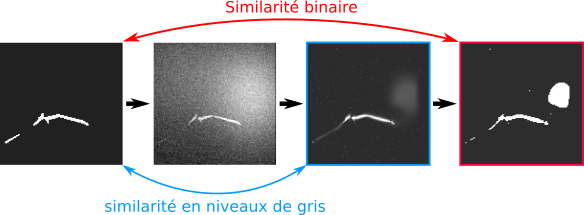
\includegraphics[width=\textwidth]{Images/similarity_procedure.png}
  \caption{On peut considérer le processus de filtrage de la manière suivante : une image de vaisseaux binaire est altérée par un processus d'acquisition (TDM ou IRM) qui produit des artefacts. Les filtres de rehaussement de vaisseaux cherchent à rétablir l'image binaire originale. Pour juger de la qualité du rehaussement, on utilise soit des mesures de similarité binaires qui nécessitent un seuillage préalable (matrice de confusion) soit une mesure en niveau de gris directement à partir de la sortie du filtre (PSNR).}
  \label{fig:custom_fig}
\end{figure}


\paragraph{Courbe ROC}

La courbe ROC (\textit{Receiving Operator Characteristic}) est une visualisation de l'évolution du taux de vrai positif en fonction du taux de faux positif au fur et à mesure des seuillages successifs appliqués au résultat des filtres. Pour rappel, le taux de vrais positifs correspond à la sensibilité et le taux de faux positifs est égal à $1-\text{spécificité}$. 

\begin{figure}[!ht]
  \centering
  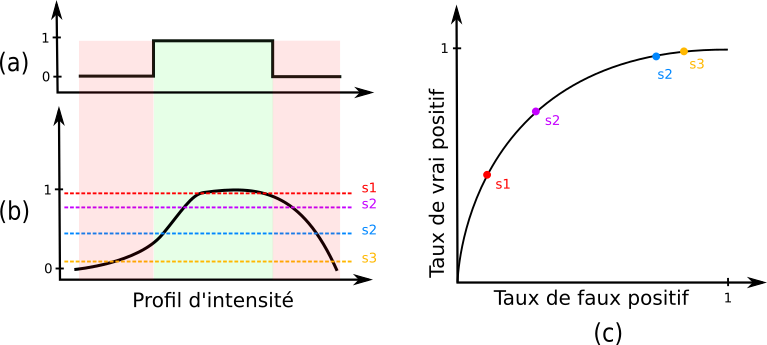
\includegraphics[width=\textwidth]{Images/roc_example.png}
  \caption{Construction d'une courbe ROC. (a) profil d'intensité de la vérité terrain. (b) profil d'intensité d'un filtre de rehaussement de vaisseaux. Selon le seuil de binarisation appliqué ($s_1,...,s_i$), on obtient des performances différentes. (c) La courbe ROC formée par le taux de vrai positif (TVP) et le taux de faux positif (TFP) en fonction du seuil résume ces variations.}
  \label{fig:roc_example}
\end{figure}


Cette courbe donne une vue globale de la performance des filtres pour l'ensemble des seuils possibles (Fig. \ref{fig:roc_example}). Elle permet le suivi de l'évolution des performances des filtres en fonction du seuil de décision choisi. Les autres métriques nous servent à quantifier les performances optimales d'un filtre. 

Une courbe ROC classique est définie par un ensemble de points $P$ dont les coordonnées sont en abscisse le TVP et en ordonnée le TFP. Cet ensemble forme généralement un pseudo arc de cercle entre les points (0,0) et (1,1) (Fig. \ref{fig:roc_example} (c)). Selon les images et les filtres appliqués, la répartition des voxels classifiés en tant que vrais ou faux positifs est variable et donc la répartition des points le long de la courbe ROC est, elle aussi, variable. Par exemple, les points qui forment la courbe ROC d'un filtre qui rehausse bien les vaisseaux sans rehausser le bruit seront répartis sur un intervalle de TFP faible, par exemple $[0,0.3]$. Un filtre qui rehausse une partie du bruit aura une répartition plus régulière sur l'axe des abscisses au fur et à mesure que le TFP augmente. 

Cette représentation de la courbe par un ensemble de points définis sur des intervalles différents demande une attention particulière pour le calcul de courbes ROC moyennes. Par exemple, si l'on possède trois courbes ROC de 200 points, chacune représentée sous la forme d'une liste de points, on ne peut pas moyenner les points en fonction des indices ($m_i = (ROC^1_{i} + ROC^2_{i} + ROC^3_{i})/3 $). Les points ne sont en effet pas échantillonnés de la même manière sur la courbe et la moyenne est faussée (Fig. \ref{fig:good_and_bad_roc}). Pour résoudre ce problème, il est nécessaire d'interpoler chaque courbe de manière à obtenir le même échantillonnage régulier sur chaque courbe. On obtient ainsi une courbe moyenne réellement représentative de la moyenne des ROC.

\begin{figure}[!ht]
  \centering
  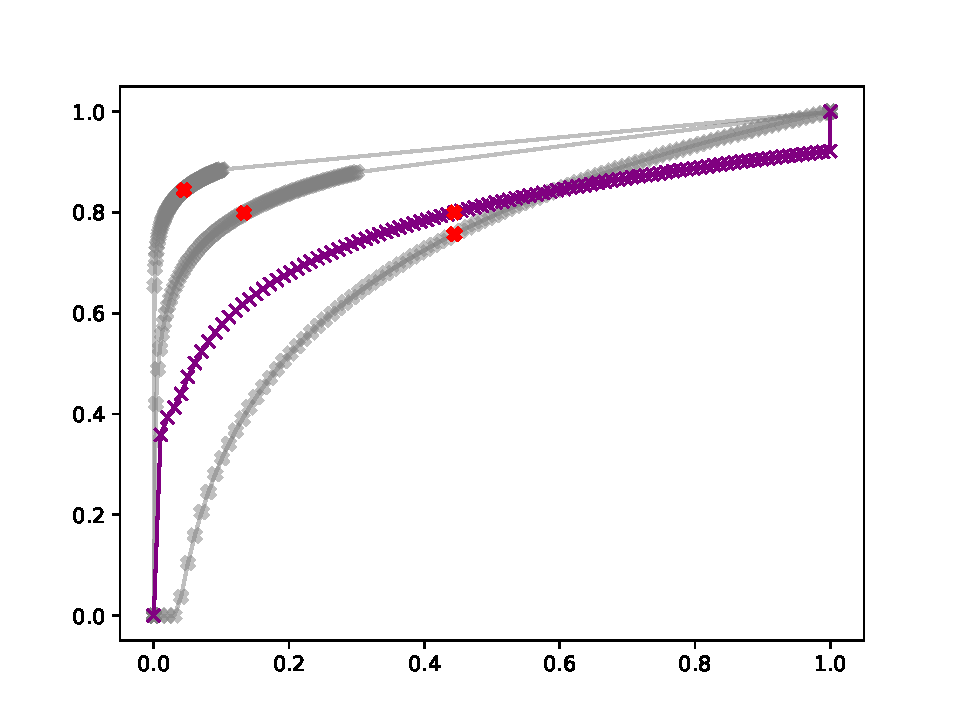
\includegraphics[height=5cm]{Images/ROC_badMean.pdf}
  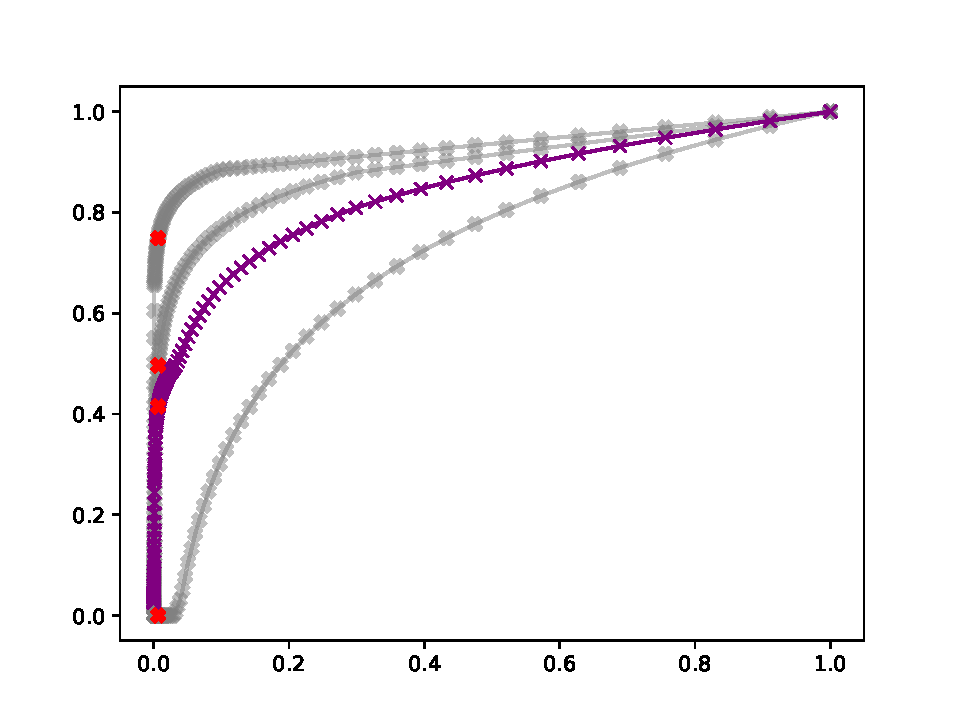
\includegraphics[height=5cm]{Images/ROC_goodMean.pdf}
  \caption{En violet, courbe ROC moyenne construite à partir des courbes ROC en gris. À gauche la courbe moyenne est construite sans interpolation. À droite, courbe ROC avec interpolation. Les points rouges sur les courbes grises sont les points ayant servi à moyenner le point rouge sur la courbe violette.}
  \label{fig:good_and_bad_roc}
\end{figure}

\section{Optimisation des paramètres}

L'un des objectifs de l'analyse des filtres de rehaussement est d'évaluer l'impact de leurs paramètres. Le choix des paramètres des filtres repose sur des considérations géométriques théoriques, mais en pratique les valeurs des paramètres à utiliser sont rarement discutées. À la place, des paramètres par défaut sont généralement proposés. C'est par exemple le cas de Frangi ($\alpha=0.5,\beta=0.5$), ou Sato $(\alpha_1=0.5,\alpha_2=2$) dont les recommandations sont reprises dans de nombreux articles sans être discutés. Pourtant, dans certains articles plus applicatifs, les paramètres utilisés par les auteurs sont différents. Par exemple, Marcan et al. \cite{Marcan2014_vessel_seg} proposent d'utiliser ($\alpha=0.3,\beta=0.7$) dans leur chaîne de segmentation,  pour l'IRM du foie. Nous avons donc voulu identifier s'il existait des règles pour le choix des valeurs des paramètres et si la recherche de paramètres optimaux était pertinente pour le rehaussement de vaisseaux.

Nous avons donc mesuré les performances d'un ensemble de jeux de paramètres pour chaque filtre et essayé de déterminer le jeu de paramètres optimal pour chaque jeu de données par rapport à une mesure et une zone d'intérêt.

Nous avons choisi d'utiliser comme métrique d'optimisation le MCC, qui mesure la similarité entre la vérité terrain binaire des vaisseaux et les volumes filtrés puis binarisés. Nous avons choisi le MCC plutôt que le Dice afin de différencier les variations de faux positifs et de faux négatifs qui ne sont pas nécessairement mesurées par le Dice (Eq. \ref{eq:Dice} et \ref{eq:MCC}). Comme le MCC est évalué sur des structures binaires, le rehaussement est simplement seuillé avant la comparaison avec la vérité terrain. Afin d'éviter de cacher des spécificités potentielles des filtres, aucun prétraitement ou post-traitement n'est réalisé sur le seuillage. Par exemple, ajouter un traitement qui consisterait à éliminer toutes les composantes connexes inférieures à 100 voxels minimiserait l'analyse de la robustesse des filtres au bruit.

La zone d'intérêt sur laquelle est calculée la métrique influence le choix du jeu de paramètres optimal. Nous avons choisi le masque \maskglobal afin que le jeu de paramètres optimal maximise la détection des vaisseaux, la  différenciation avec les autres structures, la qualité du filtrage et l'amélioration du signal des vaisseaux. Nous aurions également pu choisir de maximiser le rehaussement des vaisseaux en utilisant leur voisinage comme zone d'optimisation. Cependant, certains artefacts n'auraient pas d'impact sur le choix du jeu de paramètres. 

L'ensemble des paramètres liés aux filtres de rehaussement peuvent être classifiés en deux groupes : les paramètres d'échelles qui définissent la fenêtre permettant de capturer la taille des vaisseaux et les paramètres intrinsèques des méthodes permettant de détecter la forme des vaisseaux. Par exemple, le filtre de Frangi possède 3 paramètres liés à l'échelle et trois paramètres qui pondèrent le filtrage en fonction de la géométrie. Quand un nombre élevé de paramètres (i.e $K \gg 1$) nécessite d'être optimisé (e.g. $K=6$ pour Frangi), trouver un jeu de paramètres optimal dans l'espace à $K$ dimensions est coûteux en temps de calcul.

Dans nos expériences, nous avons choisi d'optimiser l'ensemble des paramètres en deux étapes :

\begin{itemize}
\item l'optimisation de l'échelle en utilisant des paramètres intrinsèques fixes ;
\item l'optimisation des paramètres intrinsèques en utilisant le jeu d'échelles optimales trouvé à l'étape précédente.
\end{itemize}

Les paramètres intrinsèques fixes sont ceux recommandés par les auteurs des méthodes ou sont choisis empiriquement.  Pour chaque étape, les paramètres optimaux sont définis au sens du meilleur MCC moyen dans le masque global (\maskglobal) du jeu de données entier. Cette stratégie en deux étapes peut être comparée à un choix naturel où un utilisateur commence dans un premier temps par choisir les paramètres d'échelles en se basant sur des observations des structures biologiques avant de raffiner le rehaussement (Fig. \ref{fig:flowchart_opti}).

\begin{figure}[!ht]
  \centering
  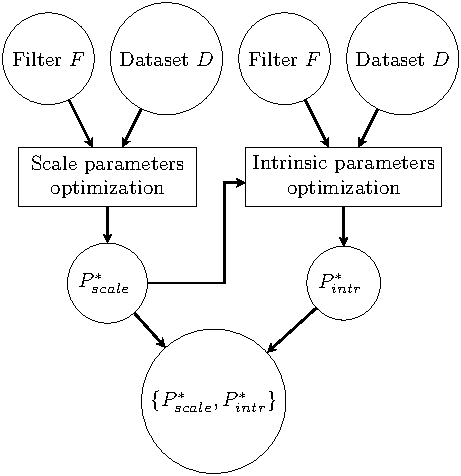
\includegraphics[height=6cm]{Images/flowchart_benchmark.pdf}
  \caption{Diagramme illustrant l'optimisation en deux temps : d'abord l'optimisation de l'échelle puis l'optimisation des paramètres intrinsèques. $\{P^*_{\acute{e}chelle},P^*_{intr}\}$ forme le jeu de paramètres optimal final.}
  \label{fig:flowchart_opti}
\end{figure}


\subsection{Méthode de calcul}
\subsubsection{Calcul du MCC moyen}

  Notre définition du MCC moyen a connu deux formulations successives afin de supprimer les biais présents dans la première définition (Fig. \ref{fig:optim_v1} et \ref{fig:optim_v2}). La première formulation présentait des défauts que nous avons corrigés dans la seconde version.
  
  Nous présentons la méthode de calcul du MCC moyen pour un  seul filtre et une seule base de données. En réalité nous avons calculé le MCC moyen de tous les jeux de paramètres pour tous les filtres sur l'ensemble des bases de données. De plus, le MCC moyen optimal est calculé pour la zone d'intérêt \maskglobal, mais une fois le jeu de paramètres optimal trouvé, la moyenne de chacune des métriques présentées précédemment est calculée pour ce jeu de paramètres dans les six zones d'intérêt. Le calcul de la moyenne de chaque métrique est effectué de la même manière que celle du MCC.    

  \paragraph{Première version}

  \begin{figure}[!ht]
    \centering
    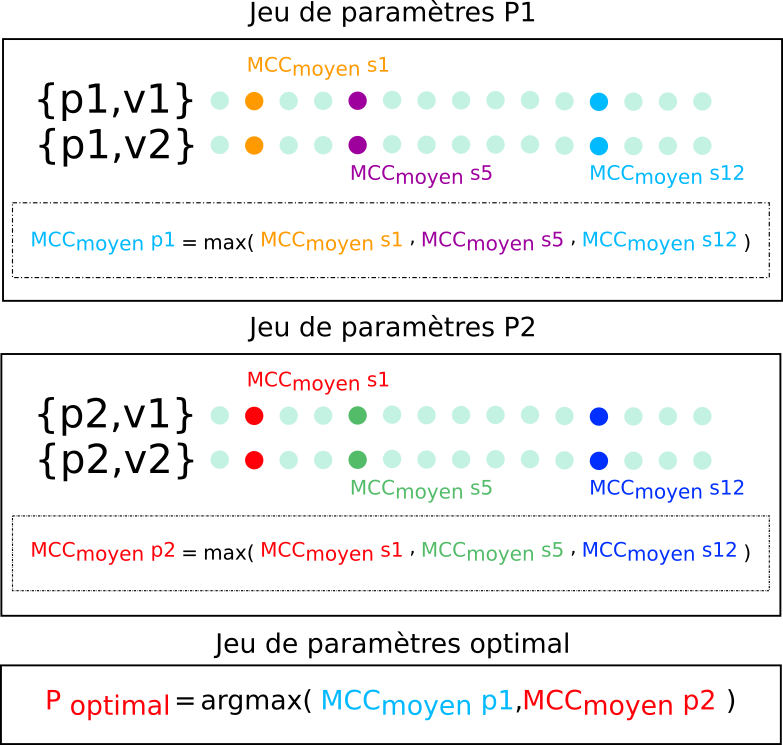
\includegraphics[width=0.80\textwidth]{Images/optim_v1.png}
    \caption{Exemple de la première version du calcul du jeu de paramètres optimal. Ici, seulement deux jeux de paramètres $P1$ et $P2$ sont appliqués à deux volumes $V1$ et $V2$. Les points correspondent aux valeurs des MCC des volumes filtrés et seuillés par le seuil $s$. Dans cette version, la moyenne s'effectue par niveaux de seuils.}
    \label{fig:optim_v1}
  \end{figure}

  Soit $F$ un filtre de rehaussement et $D$ un jeu de données de $N$ images. Soit $P$ l'ensemble des jeux de paramètres
  $\forall p \in P$, $\forall v \in D$ :
  \begin{equation}
    R_{p,v} = F_{p}(v)
  \end{equation}

  avec $R_{p,v}$ le résultat du filtrage de $v$ par $F_p$.
  Soit l'ensemble $S$ des seuillages $s$ appliqués à $R$ tels que $\forall s \in S$ :
  \begin{equation}
    RS_{p,v,s} = seuillage(R_{p,v},s) 
  \end{equation}
  Soit la valeur du MCC $MCC_{p,v,s}$ calculée pour le volume seuillé $RS_{p,v,s}$.
  Alors le MCC moyen par seuil $\overline{MCC}_{p_i,s_k}$ est défini par :
  \begin{equation}
    \overline{MCC}_{p_i,s_k} = \frac{1}{N}\sum_{v \in D} MCC_{p,v,s}
  \end{equation}
  Le meilleur MCC moyen $\overline{MCC}_{p}$ par jeu de paramètres est défini par : 
  \begin{equation}
    \overline{MCC}_{p} = \max_{s \in S} \overline{MCC}_{p,s}
  \end{equation}
  Le meilleur jeu de paramètres $p*$ est défini comme le jeu de paramètres dont le MCC moyen est maximal :
  \begin{equation}
    p* = \arg\max_{p \in P} \overline{MCC}_{p}
  \end{equation}

  Cette méthode (Fig. \ref{fig:optim_v1}), utilisée dans nos premiers travaux \cite{Lamy2020_VPH_bench} \cite{Lamy2021_RRPR} \cite{Lamy2020_ICPR} \cite{Lamy2021_ORASIS}, souffre des mêmes limitations qu'une moyenne effectuée naïvement pour calculer des courbes ROC. Elle traite en effet des rehaussements ayant des dynamiques différentes, ce qui sous-estime les résultats. 
  
  \paragraph{Deuxième version}

  \begin{figure}[!ht]
    \centering
    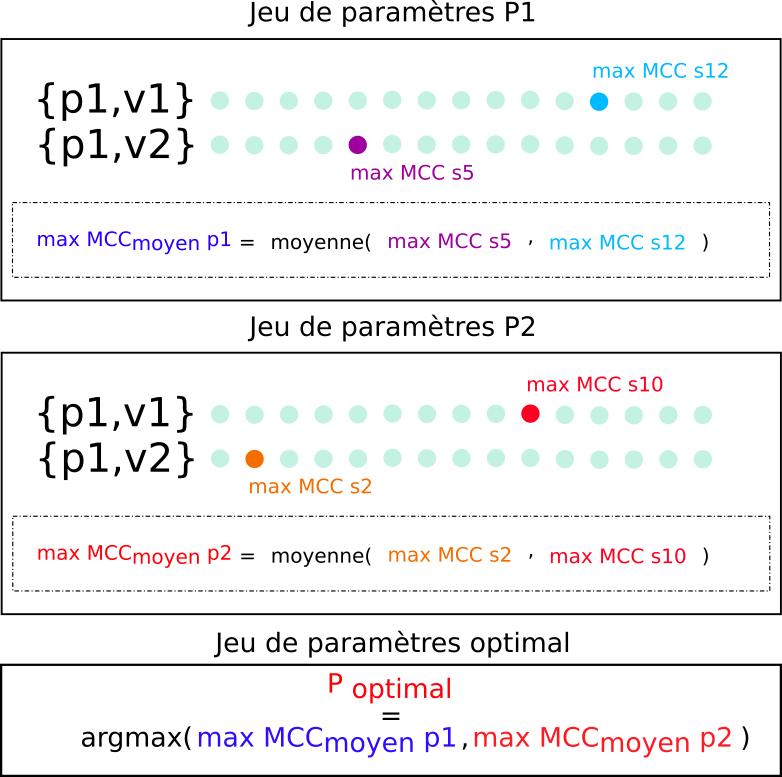
\includegraphics[width=0.80\textwidth]{Images/optim_v2.png}
    \caption{Exemple de la seconde version du calcul du jeu de paramètres optimal. Ici, seulement deux jeux de paramètres $P1$ et $P2$ sont appliqués à deux volumes $V1$ et $V2$. Les points correspondent aux valeurs des MCC des volumes filtrés et seuillés par le seuil $s$. Dans cette version, la moyenne est calculée à partir du MCC maximal obtenu par volume.}
    \label{fig:optim_v2}
  \end{figure}

  Pour la deuxième itération (Fig. \ref{fig:optim_v2}), il a été choisi de maximiser le MCC du rehaussement dès l'étape de seuillage en choisissant le seuil maximisant le MCC par volume, plutôt que de moyenner le MCC par seuil sur l'ensemble des volumes. 

  Soit $F$ un filtre de rehaussement et $D$ un jeu de données de $N$ images. Soit $P$ l'ensemble des jeux de paramètres. 
  $\forall p \in P$, $\forall v \in D$, on nomme $R_{p,v}$ le résultat du filtre de paramètres $p$ appliqué à l'image $v$:
  \begin{equation}
    R_{p,v} = F_{p}(v)
  \end{equation}
  Soit l'ensemble $S$ des seuillages appliqués à $R_{p,v}$ tel que $\forall s \in S$ 
  \begin{equation}
    RS_{p,v,s} = seuillage(R_{p,v},s) 
  \end{equation}
  Soit la valeur du MCC $MCC_{p,v,s}$ calculée pour le volume seuillé $RS_{p,v,s}$.
  Alors le MCC maximal par volume $MCC_{p_i,v_j}^{max}$ est défini par :
  \begin{equation}
    MCC_{p,v}^{max} = \max_{\forall s \in S} MCC_{p,v,s}
  \end{equation}
  Le meilleur MCC moyen $\overline{MCC}_{p_i}$ par jeu de paramètres est défini par : 
  \begin{equation}
    \overline{MCC}_{p} = \frac{1}{N} \sum_{v \in D} MCC_{p,v}^{max}
  \end{equation}
  Le meilleur jeu de paramètres $p^*$ est défini comme le jeu de paramètres dont le MCC moyen est maximal :
  \begin{equation}
    p^* = \arg\max_{p \in P} \overline{MCC}_{p}
  \end{equation}

  Dans cette itération, on choisit la procédure d'optimisation la plus favorable à chaque filtre. On tire donc le maximum des performances du pipeline de segmentation. Cette manière de procéder est utilisée aux deux étapes de l'optimisation sans changement de l'algorithme. Dans notre analyse du rehaussement, le pas appliqué entre chaque seuil est de 0.005, ce qui conduit à 201 seuils binaires. Cette méthode est utilisée dans nos travaux \cite{Lamy2022_TMI}.

  \subsection{Choix des paramètres}

Une stratégie de recherche exhaustive (\textit{grid search}) est réalisée pour l'optimisation des paramètres d'échelles $P_{\acute{e}chelle}$ et $P_{intr}$. Les conditions de cette recherche sont résumées dans les tables \ref{tab:SS_interval} et \ref{tab:SS_interval_RORPO} (paramètres d'échelles) et la table \ref{table:PS_interval} (paramètres intrinsèques).

Le choix des paramètres a été fait de manière à trouver un compromis entre temps de calcul total du banc de test, espacement des paramètres et exhaustivité. Les limites des paramètres d'échelles ont été définies en mesurant la taille des structures des troncs des réseaux vasculaires pour la limite haute et les limites de la résolution d'un pixel pour la limite basse. Une échelle inférieure à un pixel n'aurait en effet pas de sens pour les espaces gaussiens et de flux. La mesure de la taille des structures a été effectuée sur des images isotropes de résolution $[1\textrm{mm},1\textrm{mm},1\textrm{mm}]$. 

Nous avons aussi intégré des limites de distances entre deux échelles successives d'un même jeu de paramètres. Cette limite permet d'éviter les jeux de paramètres aux échelles redondantes. C'est pourquoi tout jeu de paramètres d'échelles dont la différence entre chaque échelle successive est inférieure à $\frac{1}{6}$ mm est éliminé. Pour RORPO, les tailles minimale et maximale des chemins ont été choisies empiriquement par validation visuelle. Une limite minimale à la taille entre deux chemins successifs pour un jeu de paramètres a aussi été déterminée empiriquement de manière à limiter la redondance.
 \begin{table}[!ht]
  \caption{Paramètres d'échelle pour les filtres utilisant un espace d'échelles basé sur le diamètre :  Frangi, Sato, Meijering, Jerman, Zhang, OOF. Les conditions  assurent que l'écart entre deux échelles successives $\sigma_i$ et $\sigma_j$ soit supérieur à la résolution d'un voxel.}
  \label{tab:SS_interval}
  \begin{center}
    \begin{tabular}{  l  c  c  c }
      \hline
      \multicolumn{4}{c}{ Ircad et VascuSynth }\\
      \hline
      Paramètres & Intervalle & Pas & Conditions \\
      \hline
      $\sigma_{\min}$ & $[0.4,1.8]$ & $0.4$ & \\
      $\sigma_{\max}$ & $[1.4,3.4]$  & $0.4$ & $\sigma_{i} - \sigma_{j} > \frac{1}{6}$ mm \\ 
      Nombre d'échelles & $[\![3,4]\!]$ & $1$ & \\
      \hline
      \hline
      \multicolumn{4}{c}{ Bullitt }\\
      \hline
      Paramètres & Intervalle & Pas & Conditions \\
      \hline
      $\sigma_{\min}$ & $[0.2,1.6]$ & $0.4$ & \\
      $\sigma_{\max}$ & $[1.2,3.2]$  & $0.4$ & $\sigma_{i} - \sigma_{j} > \frac{1}{6}$ mm \\ 
      Nombre d'échelles & $[\![3,4]\!]$ & $1$ & \\
      \hline
    \end{tabular}
  \end{center}
\end{table}
\begin{table}[!ht]
  \caption{ Paramètres d'échelle pour RORPO sans le paramètre de dilatation. Les conditions d'espacement assurent que deux échelles successives $i$ et $j$  ne soient pas similaires et que le chemin de taille maximal $\acute{e}chelle_{max}$ ne dépasse pas une certaine taille.}
  \label{tab:SS_interval_RORPO}
  \begin{center}
    \begin{tabular}{  l  c  c  c }
      \hline
      \multicolumn{4}{c}{Ircad}\\
      \hline
      Paramètres & Intervalle & Pas & Conditions \\
      \hline
      Échelle min. & $[30,150]$ & $10$ & \\
      Facteur & $[1.1,1.6]$ & $0.1$ & $20 < \textrm{échelle}_{i} - \textrm{échelle}_{j} \textrm{~et~} \textrm{échelle}_{max} < 200 $ \\ 
      Nb. d'échelles & $[\![2,4]\!]$ & $1$ & \\
      \hline
      \hline
      \multicolumn{4}{c}{Bullitt}\\
      \hline
      Paramètres & Intervalle & Pas & Conditions \\
      \hline
      Échelle min. & $[30,90]$ & $10$ & \\
      
      Facteurs & $[1.1,1.5]$  & $0.1$ & $ 20 < \textrm{échelle}_{i} - \textrm{échelle}_{j} \textrm{~et~} \textrm{échelle}_{max} < 200$ \\
      Nb. échelles & $[\![2,4]\!]$ & $1$ & \\
      \hline
      \hline
      \multicolumn{4}{c}{VascuSynth}\\
      \hline
      Paramètres & Intervalle & Pas & Conditions \\
      \hline
      Échelle min. & $[10,90]$ & $10$ & \\
      
      Facteur & $[1.1,1.5]$  &  $0.1$ & $ 9 < \textrm{échelle}_{i} - \textrm{échelle}_{j} \textrm{~et~} \textrm{échelle}_{max} < 100$ \\
      
      Nb. d'échelles & $[\![2,4]\!]$ & $1$ & \\
      \hline
    \end{tabular}
  \end{center}
\end{table}
\begin{table}[!ht]
  \caption{Paramètres intrinsèques (Meijering et RORPO n'ont pas de paramètre intrinsèque).}
  \label{table:PS_interval}
  \begin{center}
    \begin{tabular}{  l  c  c  c }
      \hline
      Filtres & Paramètres & Intervalle & Pas \\
      \hline
      Frangi & $\alpha$ & $[0.2,1.0]$ & $0.2$ \\
      ---       & $\beta$ & $[0.2,1.0]$ & $0.2$  \\
      ---       & $C$& $[0,60]$ & $30$ \\
      Sato & $\alpha_{1}$ & $[0.2,1.0]$ & $0.2$ \\
      ---     & $\alpha_{2}$ & $[1,2]$ & $0.2$ \\
      OOF & $\sigma$ & $[0.1,1.0]$ & $0.1$ \\
      Jerman & $\tau$ & $[0.1,1.0]$ & $0.1$ \\
      Zhang & $\tau$& $[0.1,1.0]$ & $0.1$ \\
      \hline
    \end{tabular}
  \end{center}
\end{table}
  
Au total, 41 jeux de paramètres d'échelles sont testés pour les filtres hessiens et OOF. Respectivement 32, 44 et 51 jeux de paramètres sont testés pour RORPO sur l'Ircad, VascuSynth et Bullitt. Pour les paramètres intrinsèques, 10 jeux de paramètres sont testés pour Jerman, Zhang et OOF. 75 jeux de paramètres sont testés pour Frangi et 30 pour Sato.
\section{Résultats}
Dans cette section, nous présentons et discutons des résultats quantitatifs et qualitatifs des différents filtres. En plus des sept filtres présentés précédemment, nous ajoutons un filtre témoin. Le témoin est un simple filtre de mise à l'échelle des intensités afin que l'image d'entrée soit normalisée. L'image normalisée est ensuite seuillée de la même manière que pour les filtres de rehaussement. On obtient de cette manière un seuillage optimisé qui sert de base à la comparaison des performances des filtres.

Dans la suite, nous commençons par analyser les résultats des filtres dans le masque global \maskglobal. Puis, nous discutons des résultats obtenus sur les masques vasculaires \maskvascular, \maskvesselLarge, \maskvesselMedium, \maskvesselSmall. Enfin, nous exposons les résultats obtenus au niveau des bifurcations.
\subsection{Résultats globaux}
\begin{figure}[!ht]
  \begin{subfigure}[t]{0.78\textwidth}
    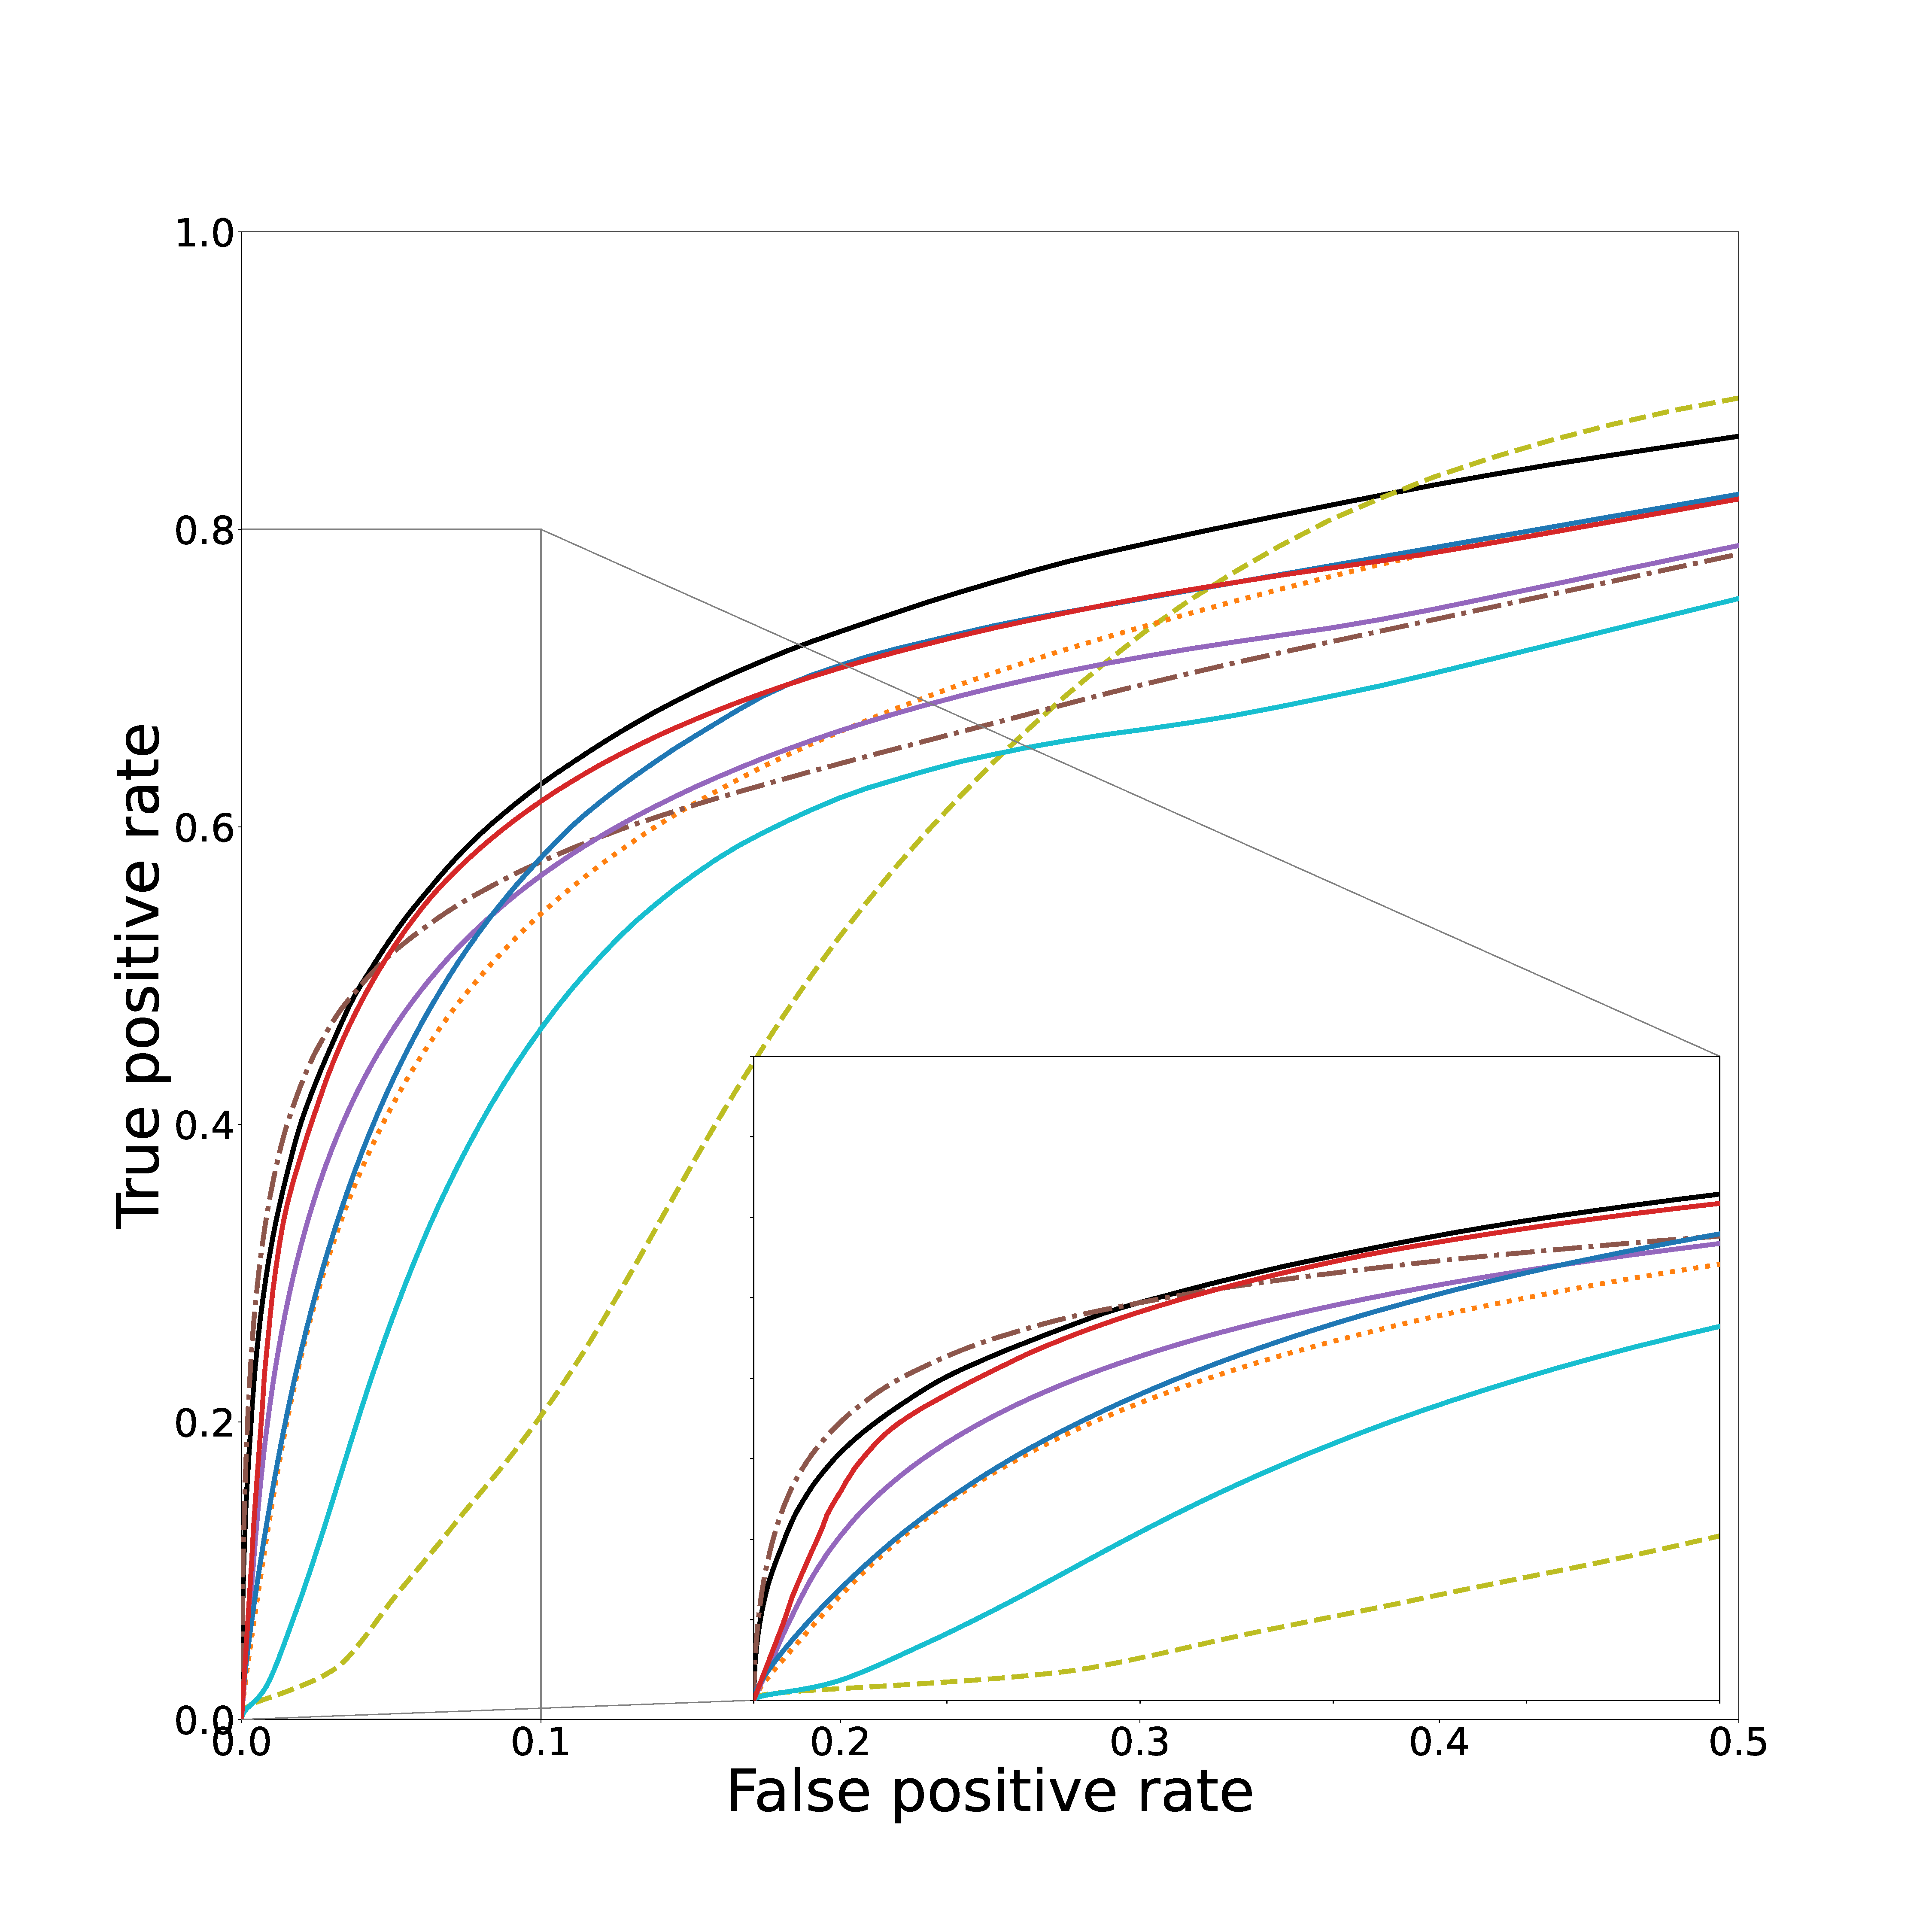
\includegraphics[width=\textwidth,clip = true, trim  =  125 125 180 200]{Images/Ircad_ROC.pdf}  
  \end{subfigure}
  \begin{subfigure}[t]{0.2\textwidth}
      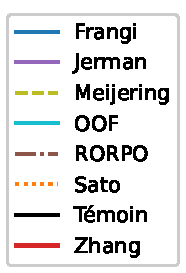
\includegraphics[width=\textwidth,clip = true]{Images/standAloneLegend.pdf}
  \end{subfigure}
  \caption{Courbe ROC moyenne des sept filtres de rehaussement pour le jeu de l'Ircad. Un zoom est effectué sur la partie gauche de la courbe ROC.}
  \label{fig:Ircad_ROC}
\end{figure}
\begin{figure}[!ht]
  \captionsetup[subfigure]{justification=centering}
  \centering
  \begin{subfigure}[t]{0.78\textwidth}
    \centering
  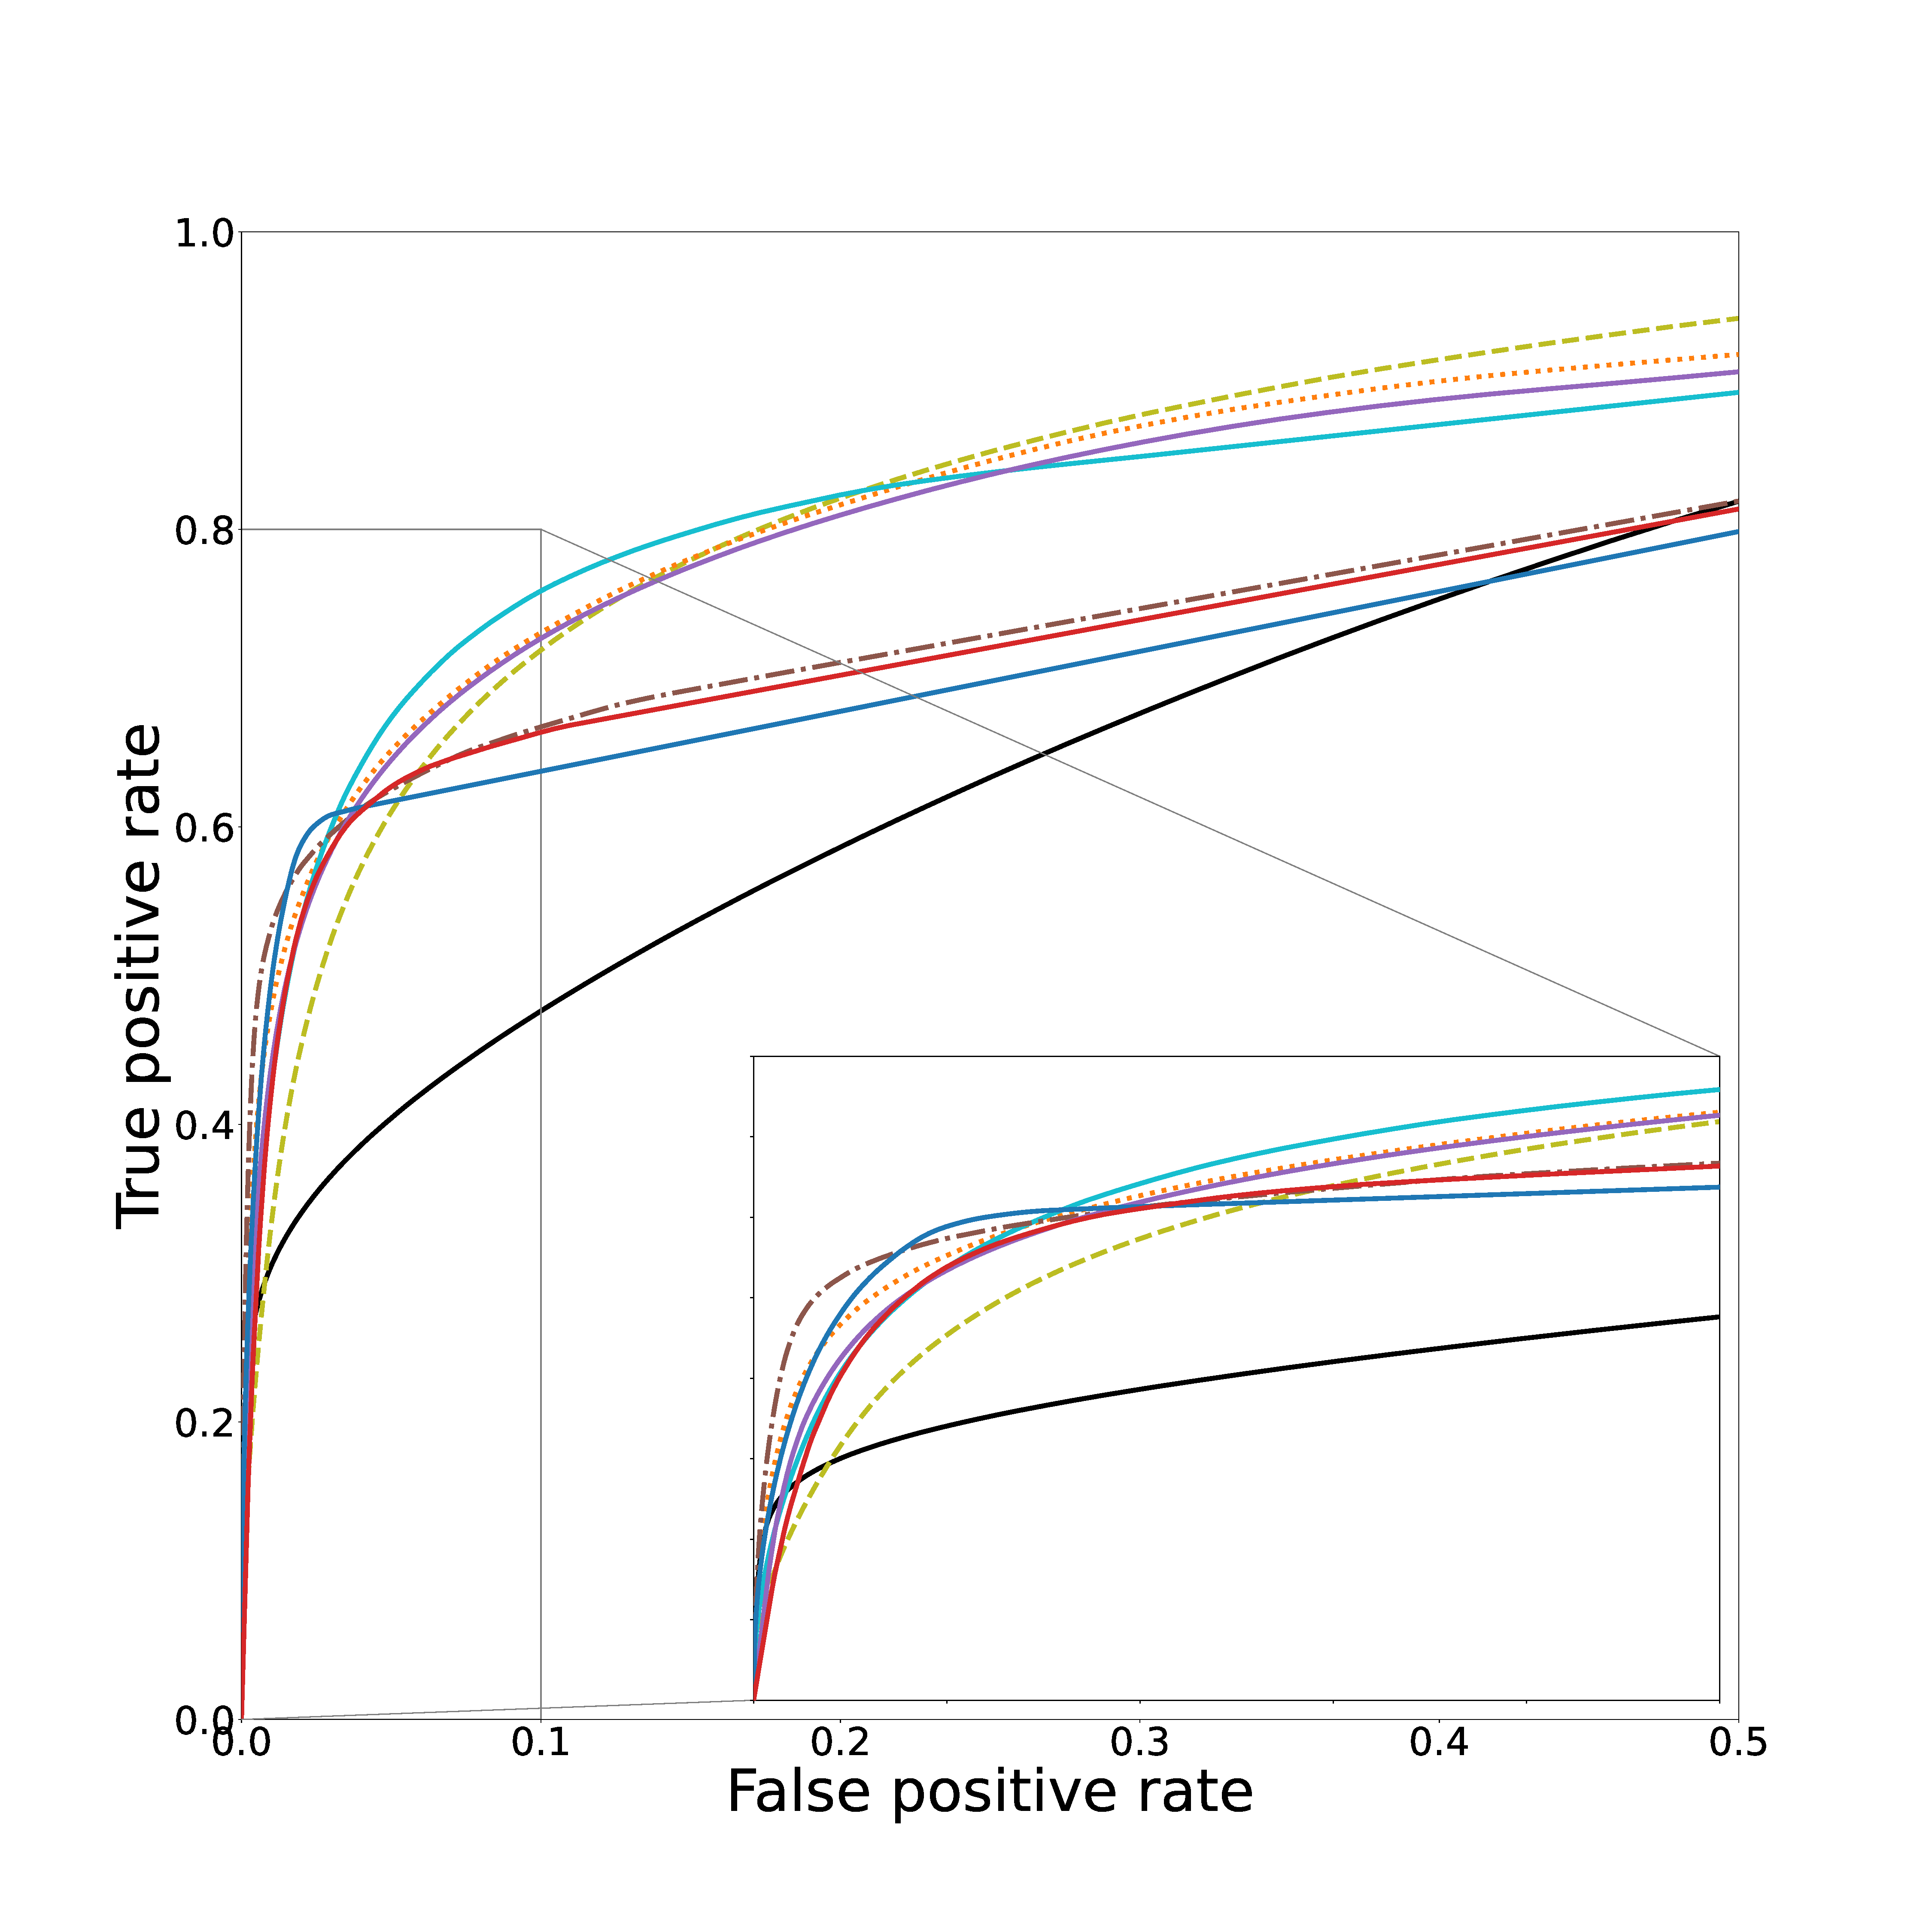
\includegraphics[width=\textwidth,clip = true, trim  =  125 125 180 200]{Images/Bullitt_ROC.pdf}
  \end{subfigure}
  \begin{subfigure}[t]{0.2\textwidth}
    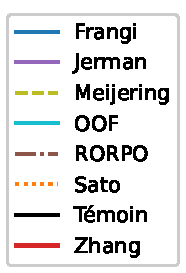
\includegraphics[width=\textwidth,clip = true]{Images/standAloneLegend.pdf}
  \end{subfigure}
  \caption{Courbe ROC moyenne des sept filtres de rehaussement pour Bullitt. Un zoom est effectué sur la partie gauche de la courbe ROC.}
\end{figure}
\begin{figure}[!ht]
  \begin{subfigure}[t]{0.78\textwidth}
    \centering
  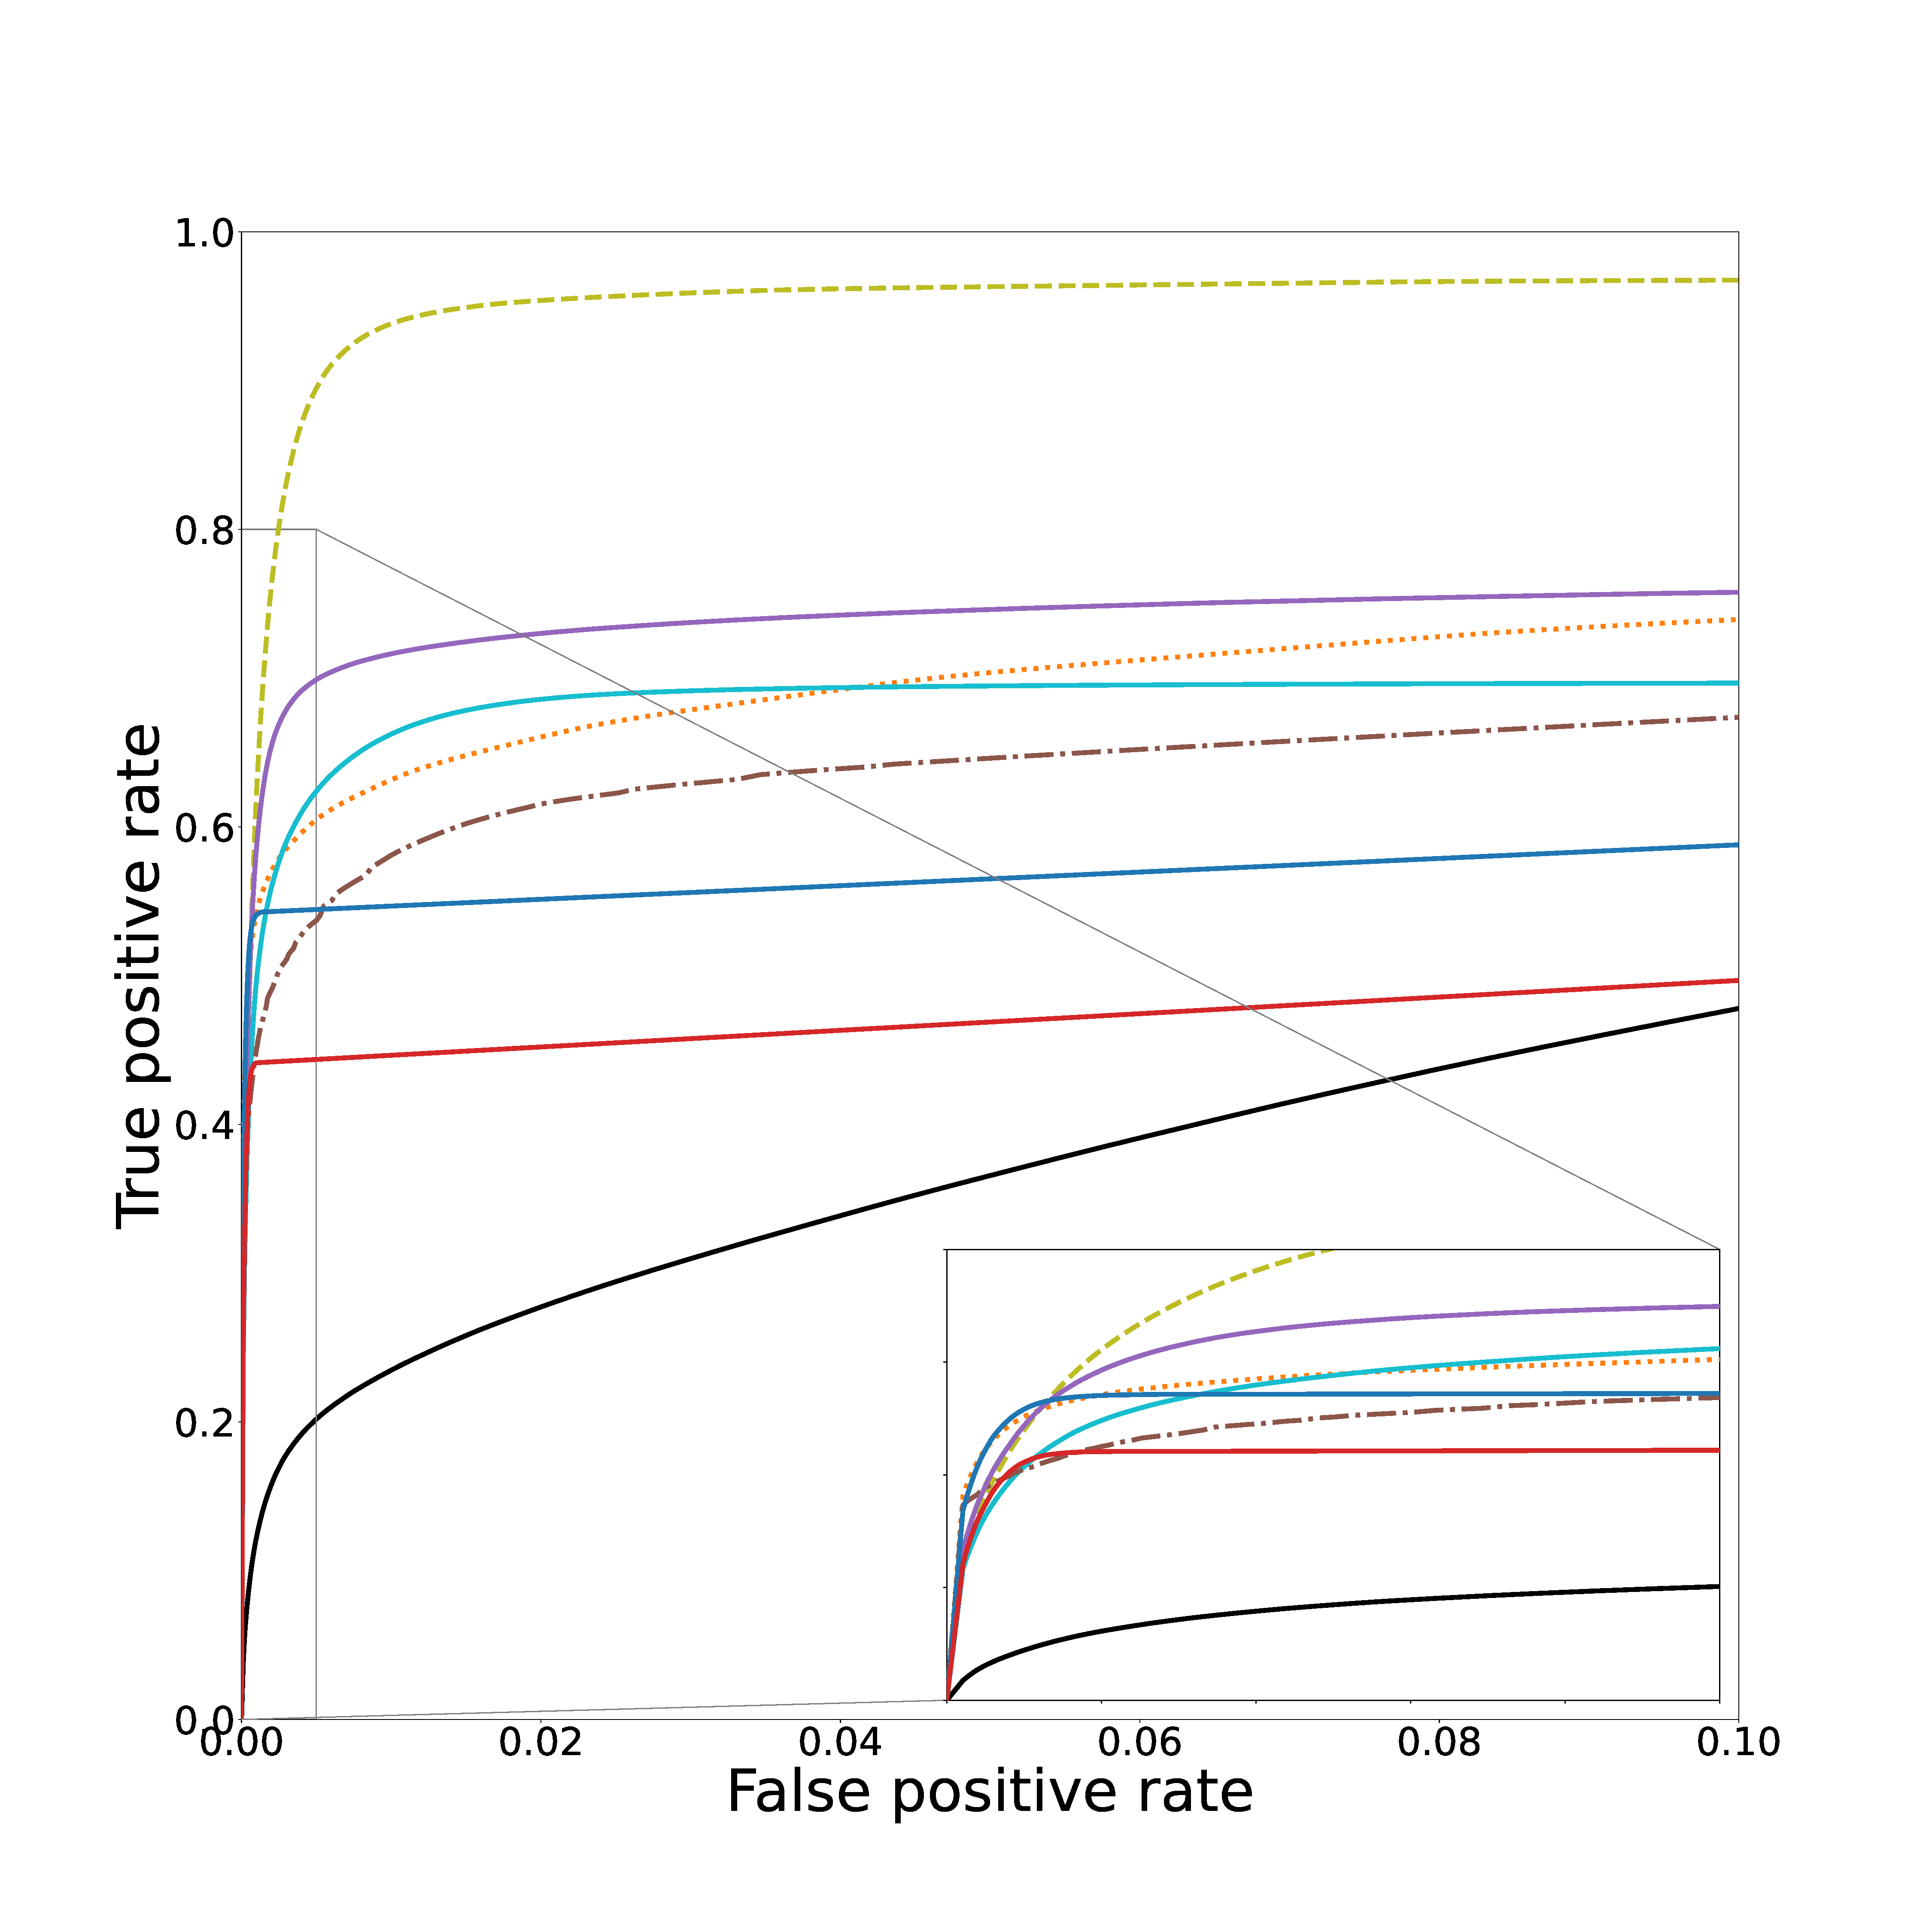
\includegraphics[width=\textwidth,clip = true, trim  =  125 125 180 200]{Images/Vascu_2_ROC.pdf}
\end{subfigure}
\begin{subfigure}[t]{0.2\textwidth}
  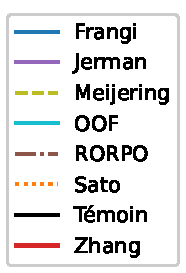
\includegraphics[width=\textwidth,clip = true]{Images/standAloneLegend.pdf}
\end{subfigure}
\caption{Courbe ROC moyenne des sept filtres de rehaussement pour VascuSynth $\sigma=2$. Un zoom est effectué sur la partie gauche de la courbe ROC.}
\end{figure}
\begin{figure}[!ht]
  \begin{subfigure}[t]{0.78\textwidth}
    \centering
  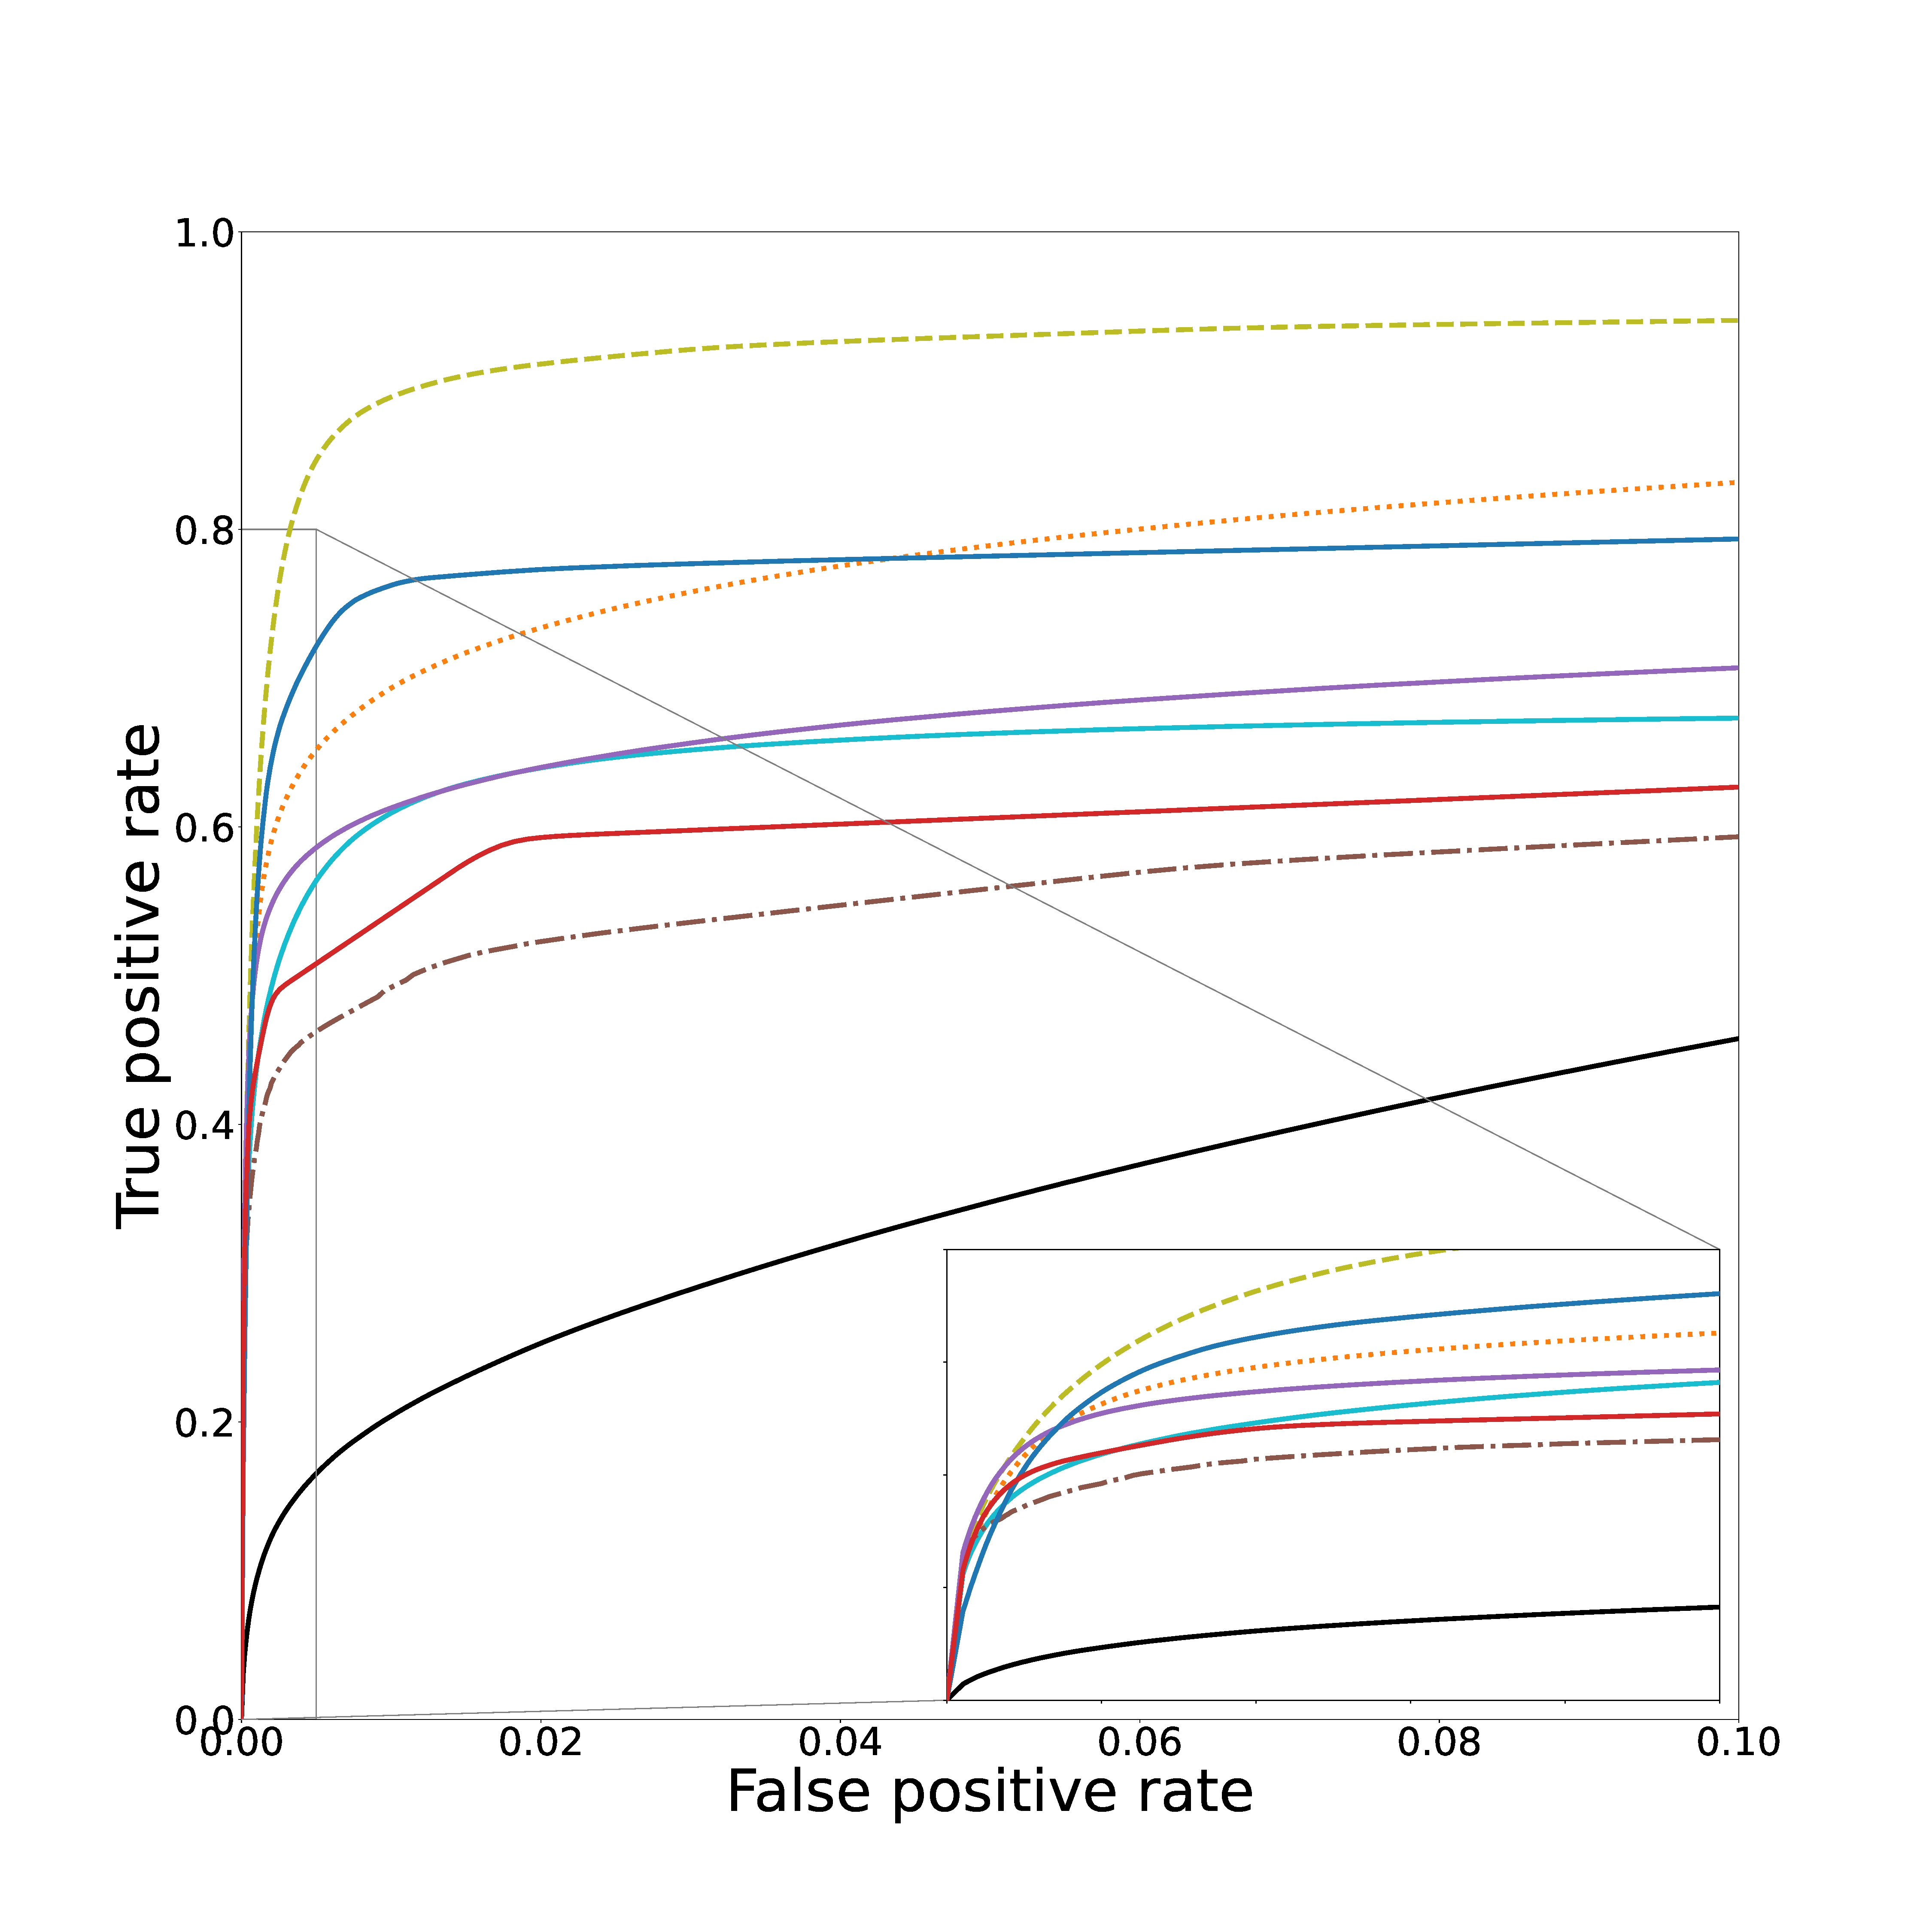
\includegraphics[width=\textwidth,clip = true, trim  =  125 125 180 200]{Images/Vascu_4_ROC.pdf}
\end{subfigure}
\begin{subfigure}[t]{0.2\textwidth}
  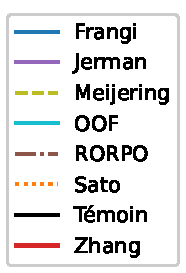
\includegraphics[width=\textwidth,clip = true]{Images/standAloneLegend.pdf}
\end{subfigure}
\caption{Courbe ROC moyenne des sept filtres de rehaussement pour VascuSynth $\sigma=4$. Un zoom est effectué sur la partie gauche de la courbe ROC.}
\end{figure}
\begin{figure}[!ht]
  \begin{subfigure}[t]{0.78\textwidth}
    \centering
    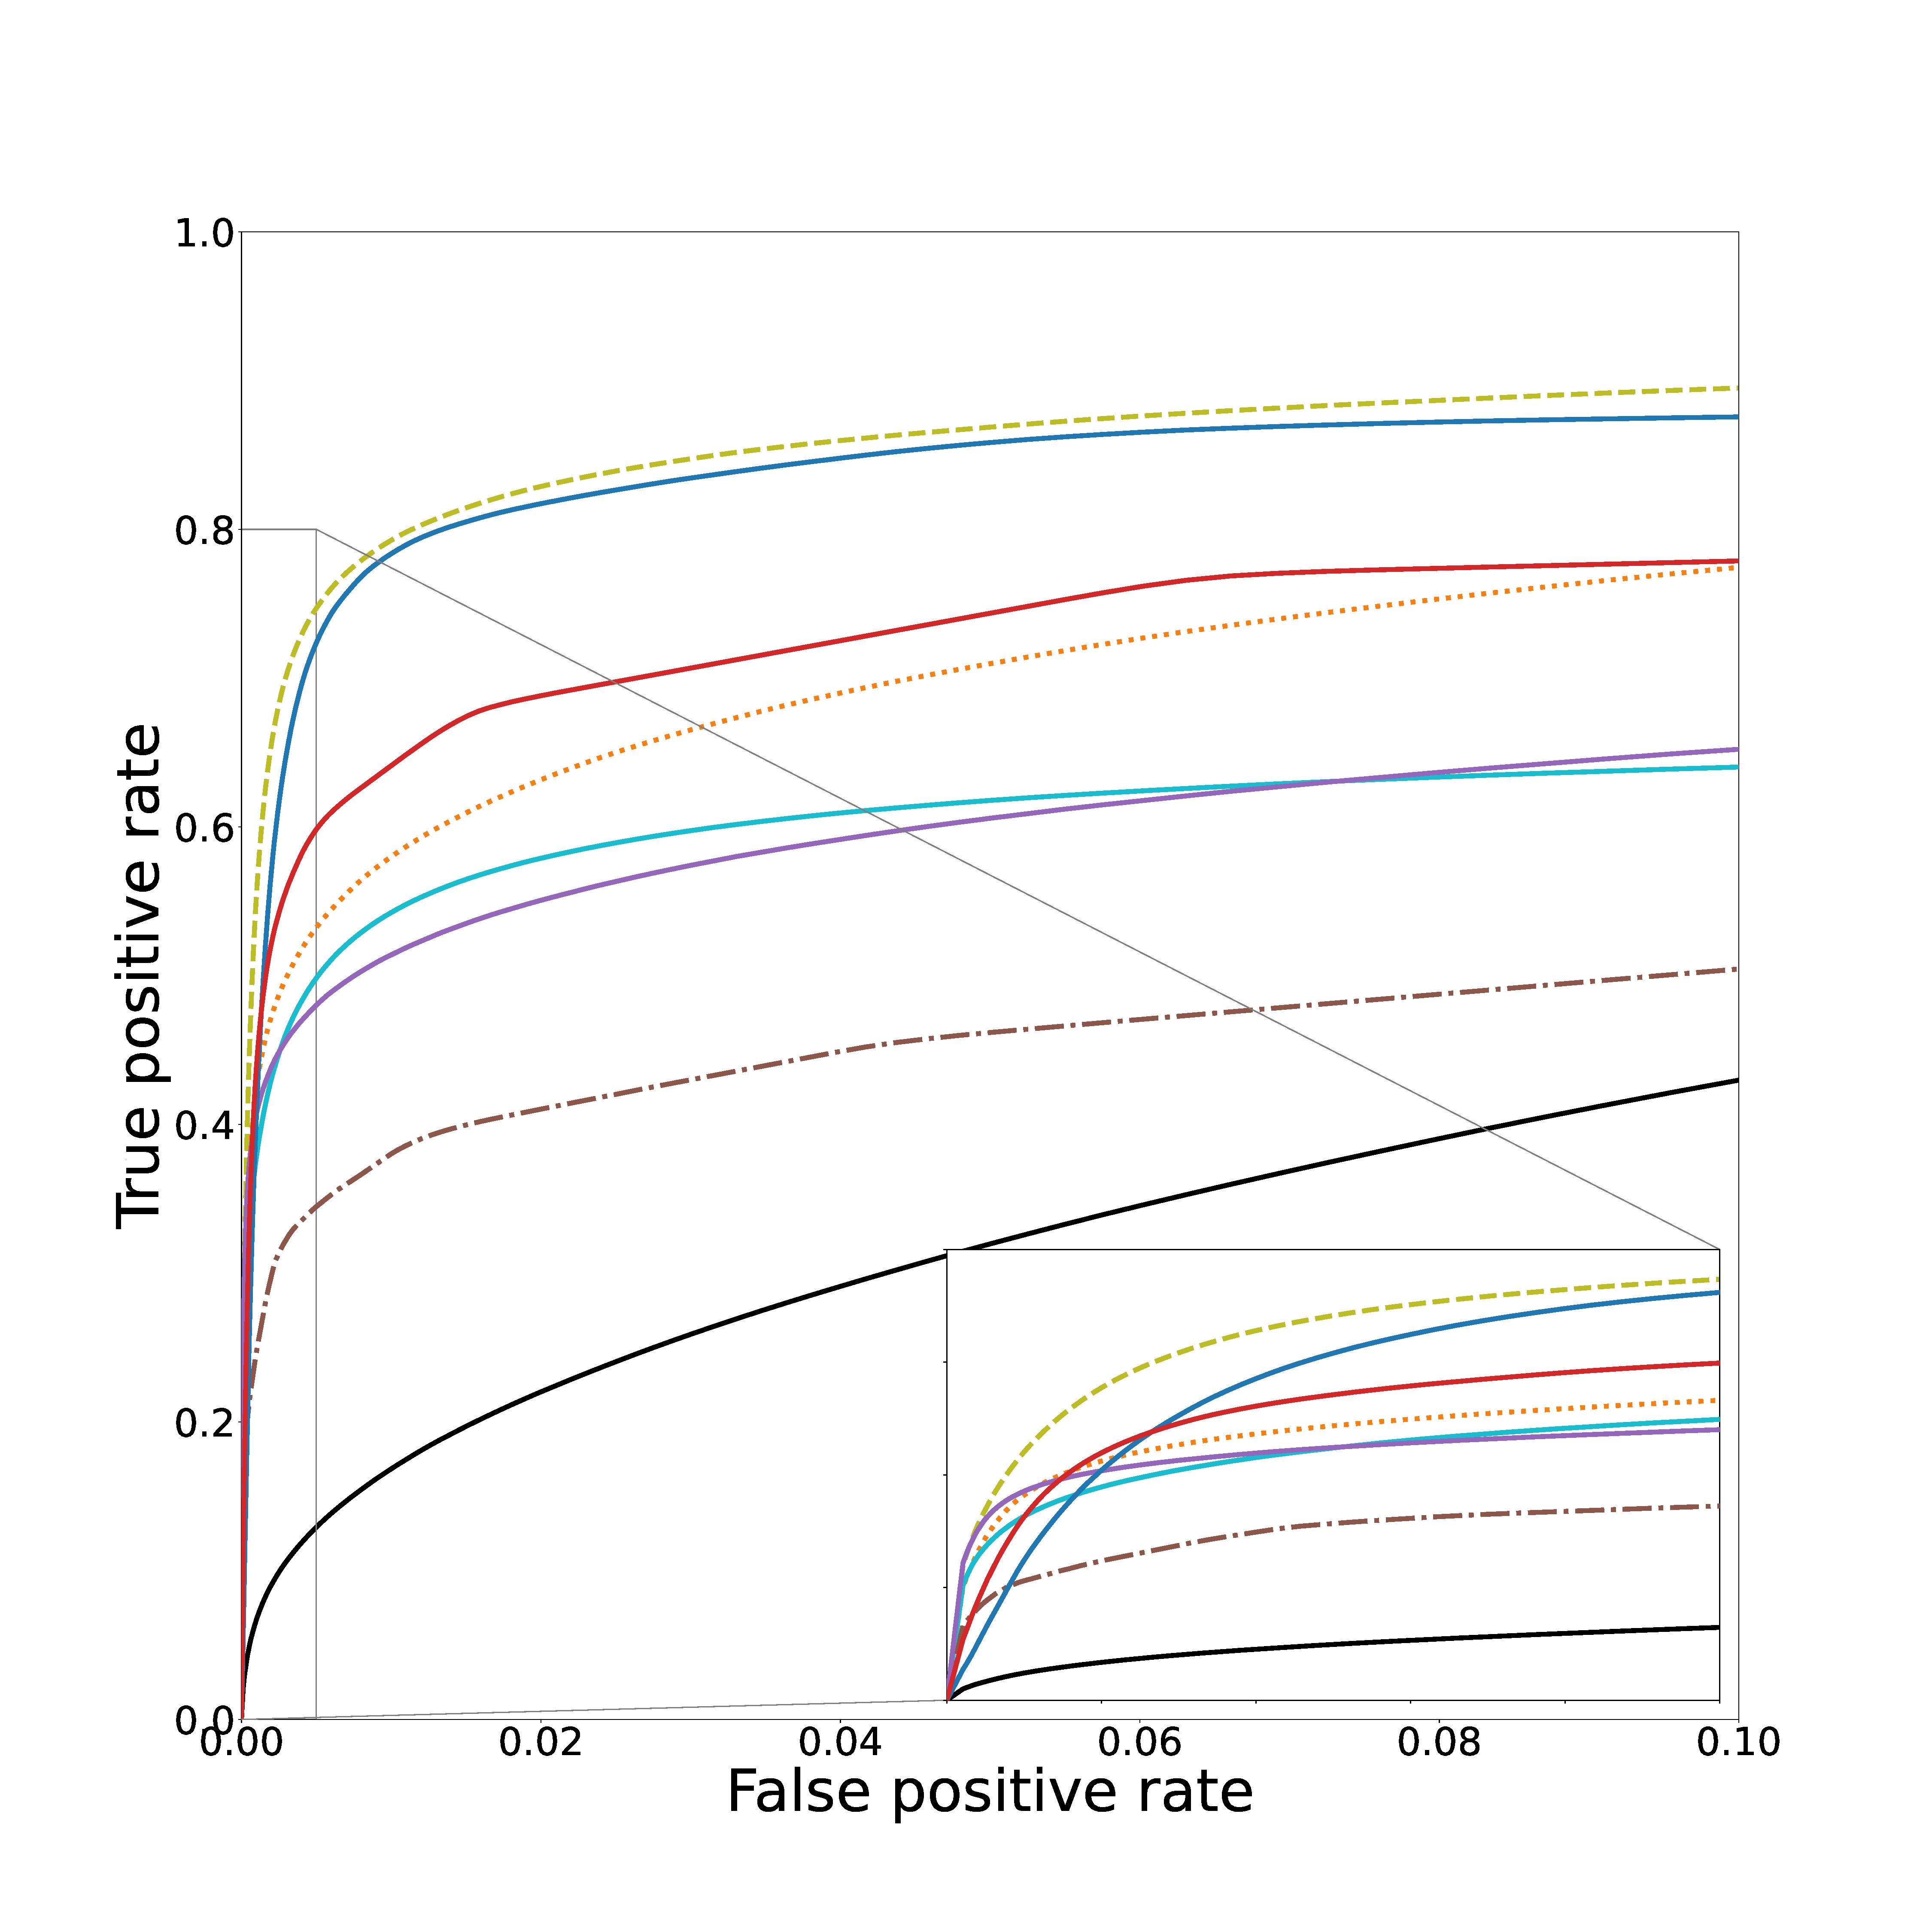
\includegraphics[width=\textwidth,clip = true, trim  =  125 125 180 200]{Images/Vascu_6_ROC.pdf}
\end{subfigure}
\begin{subfigure}[t]{0.2\textwidth}
  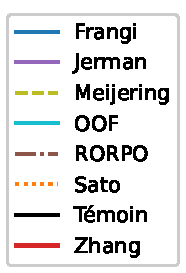
\includegraphics[width=\textwidth,clip = true]{Images/standAloneLegend.pdf}
\end{subfigure}
\caption{Courbe ROC moyenne des sept filtres de rehaussement pour VascuSynth $\sigma=6$.}
  \label{fig:Vascu6_ROC}
\end{figure}

\paragraph{Ircad}
\begin{table}[!ht]
  \begin{center}
      \caption{Résultats quantitatifs (moyenne $\pm$ écart-type) dans le masque global \maskglobal sur le jeu de données de l'Ircad.}
      \label{tab:quantitative results Ircad}
      \begin{tabular}{lccc}
          \hline
          & MCC & Dice & PSNR \\ 
          \hline
          Témoin	    & $ 0.452 \pm 0.129	$ & $ \tbf{0.468} \pm	0.126 $ & $	9.352  \pm  1.247 $ \\
          Frangi	    & $ 0.355 \pm 0.075	$ & $ 0.392 \pm	0.074 $ & $	19.899 \pm 	1.624 $ \\
          Jerman	    & $ 0.382 \pm 0.060	$ & $ 0.415 \pm	0.059 $ & $	18.926 \pm 	1.186 $ \\
          Meijering   & $ 0.232 \pm 0.036	$ & $ 0.241 \pm	0.050 $ & $	19.079 \pm 	1.392 $ \\
          OOF	        & $ 0.277 \pm 0.049	$ & $ 0.316 \pm	0.055 $ & $	19.728 \pm 	1.575 $ \\
          RORPO	      & $ \tbf{0.475} \pm 0.073	$ & $ 0.477 \pm	0.076 $ & $	\tbf{20.349} \pm 	1.687 $ \\
          Sato	      & $ 0.340 \pm 0.056	$ & $ 0.380 \pm	0.057 $ & $	19.915 \pm 	1.633 $ \\
          Zhang	      & $ 0.434 \pm 0.085	$ & $ 0.462 \pm	0.079 $ & $	20.274 \pm 	1.648 $ \\
    
          \hline
      \end{tabular}  
      \end{center}    
\end{table}
En observant les résultats présentés en table \ref{tab:quantitative results Ircad}, on peut remarquer que globalement, le MCC et le Dice de tous les filtres appliqués sur les images de foies de l'Ircad sont faibles (inférieurs à 0.5). Ce résultat était attendu puisque nous avons réduit notre chaîne de traitement au minimum. Cependant, ce résultat justifie quantitativement le fait qu'un filtre seul ne peut se substituer à une méthode de segmentation complète.

Qualitativement (Fig. \ref{fig:qualitative results Ircad}), tous les filtres excepté RORPO produisent des faux positifs sur les bords du foie. Meijering semble produire les moins bons résultats en rehaussant à la fois fortement les bords et le bruit dans les tissus. En comparaison, le seuillage, permet de bien récupérer les vaisseaux larges, mais l'on observe une augmentation des déconnexions au fur et à mesure que les vaisseaux deviennent de plus en plus petits. 

Quantitativement, RORPO propose les meilleurs résultats avec un MCC de $0.475$. Le témoin remporte le second meilleur MCC ($0.452$). Le fait qu'un simple seuillage produise de meilleurs résultats que la plupart des filtres sur des images TDM injectées peut paraître surprenant. Cependant, ces résultats sont à pondérer par le fait que les petits et moyens vaisseaux sont absents du seuillage témoin dans une proportion bien plus large que pour les filtres de rehaussement. En effet, tous les filtres ont des résultats supérieurs à la référence pour les vaisseaux petits et moyens.  

Zhang produit le troisième meilleur résultat (MCC = $0.434$), alors que OOF (MCC = $0.277$) et Meijering (MCC = $0.231$) présentent les performances les plus faibles. Les meilleurs filtres (RORPO et Zhang) obtiennent ces performances par des stratégies différentes. La précision de RORPO est élevée ($0.666$) avec une sensibilité moyenne ($0.379$). Au contraire, Zhang présente une sensibilité importante ($0.435$) en contrepartie d'une précision plus faible ($0.515$).

Nous rappelons que ces résultats sont basés sur le meilleur jeu de paramètres moyen pour l'ensemble des volumes du jeu de données. Le processus d'optimisation produit donc un rehaussement qui est le compromis entre rehausser au maximum les vaisseaux, limiter le bruit et limiter le rehaussement des structures qui ne sont pas des vaisseaux (telles que les bords du foie). 
\begin{figure}[!ht]
  \captionsetup[subfigure]{justification=centering}
  \begin{subfigure}[t]{0.32\textwidth}
  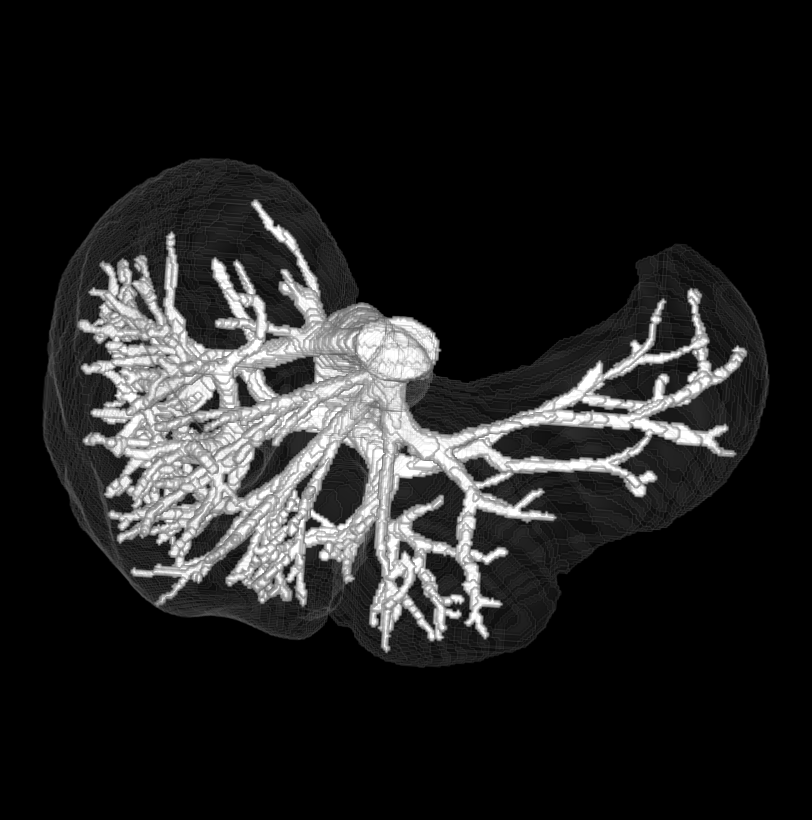
\includegraphics[clip = true, trim  =  10 150 10 150, height=3cm,width=4cm]{Images/Ircad_GT.png}
  \caption{Vérité terrain}
  \end{subfigure}
  \begin{subfigure}[t]{0.32\textwidth}
  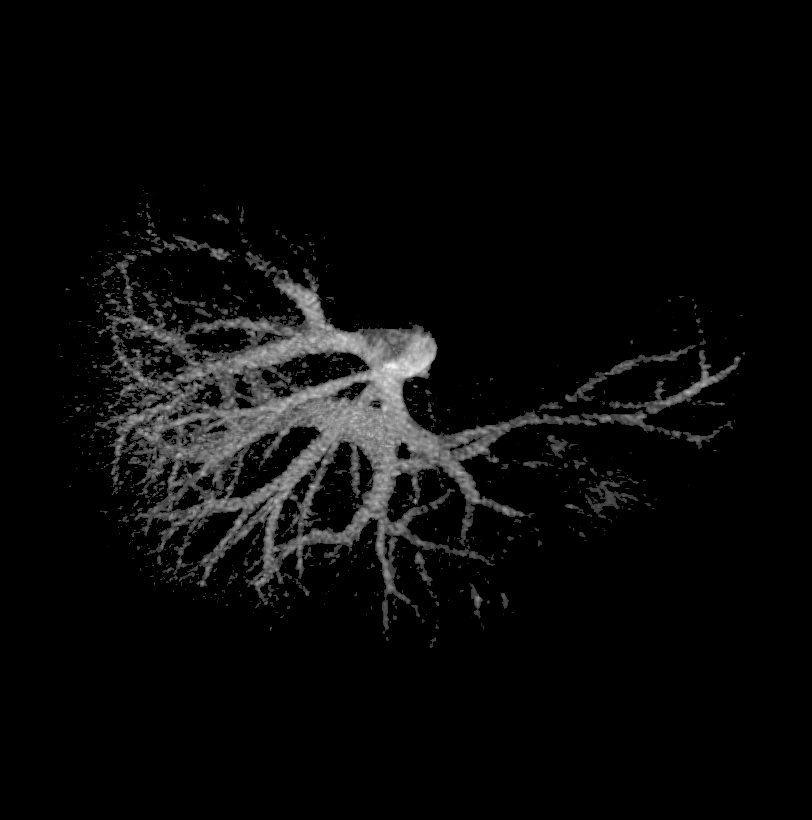
\includegraphics[clip = true, trim  =  10 150 10 150, height=3cm,width=4cm]{Images/Ircad_Baseline.png}
  \caption{Témoin}
  \end{subfigure}
  \begin{subfigure}[t]{0.32\textwidth}
  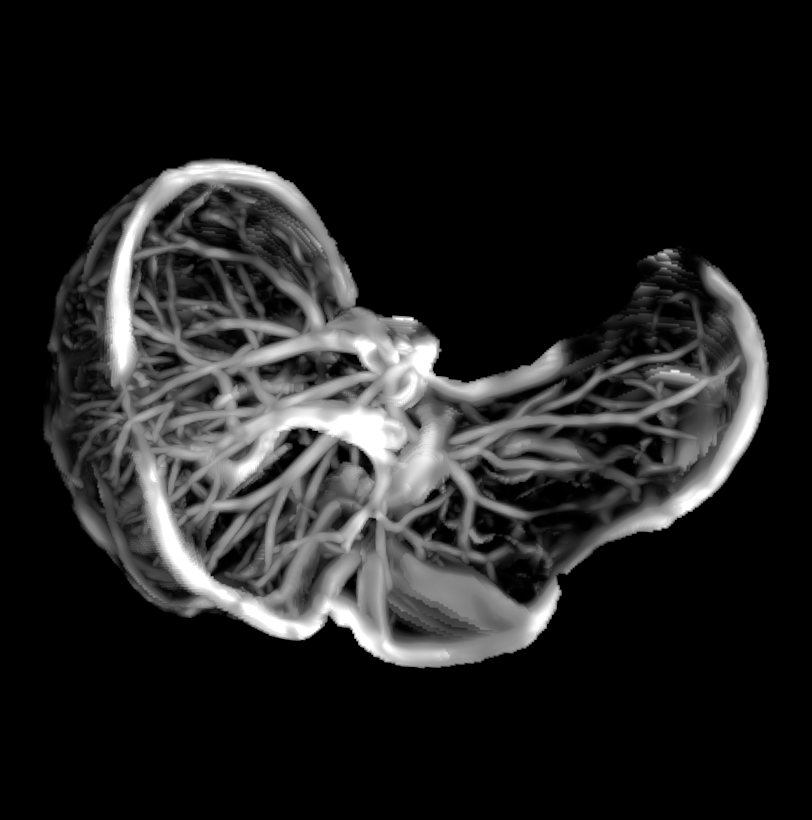
\includegraphics[clip = true, trim  =  10 150 10 150, height=3cm,width=4cm]{Images/Ircad_Frangi.png}
  \caption{Frangi}
  \end{subfigure}
  \begin{subfigure}[t]{0.32\textwidth}
  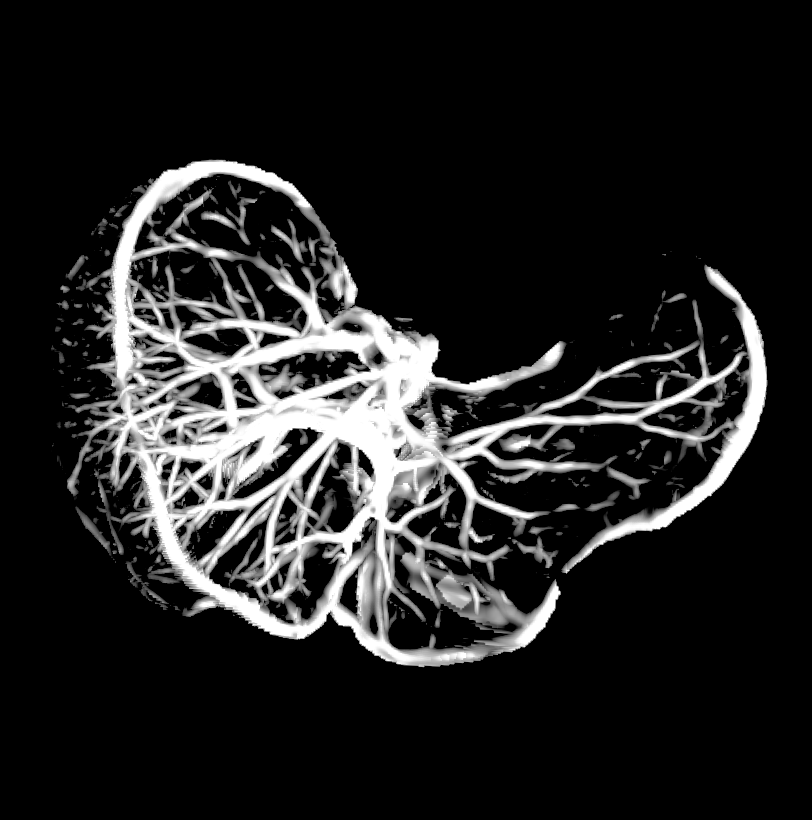
\includegraphics[clip = true, trim  =  10 150 10 150, height=3cm,width=4cm]{Images/Ircad_Jerman.png}
  \caption{Jerman}
  \end{subfigure}
  \begin{subfigure}[t]{0.32\textwidth}
  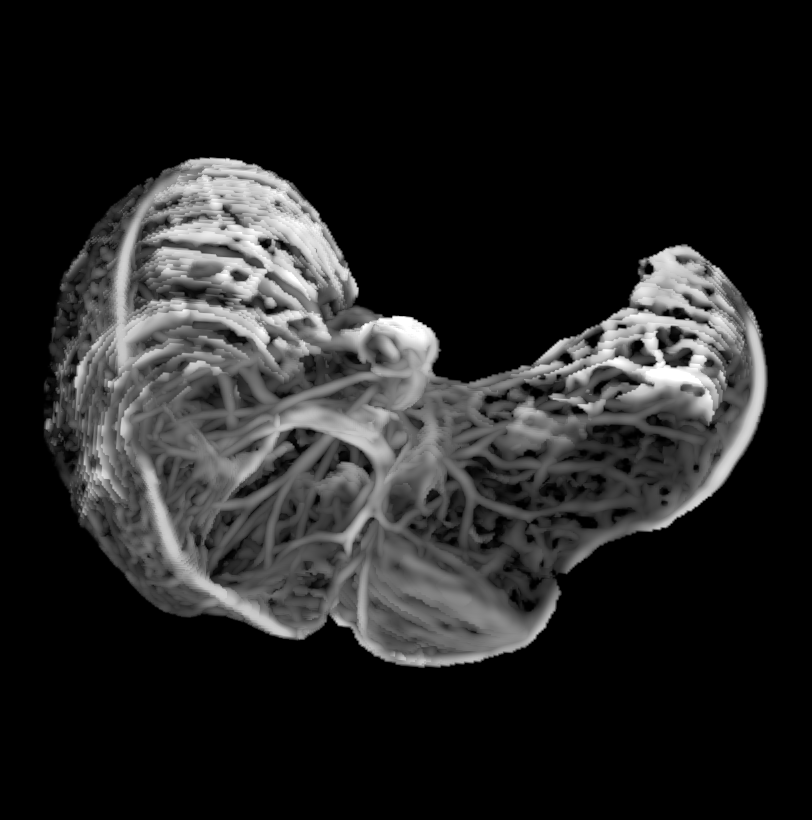
\includegraphics[clip = true, trim  =  10 150 10 150, height=3cm,width=4cm]{Images/Ircad_OOF_GM.png}
  \caption{OOF}
  \end{subfigure}
  \begin{subfigure}[t]{0.32\textwidth}
  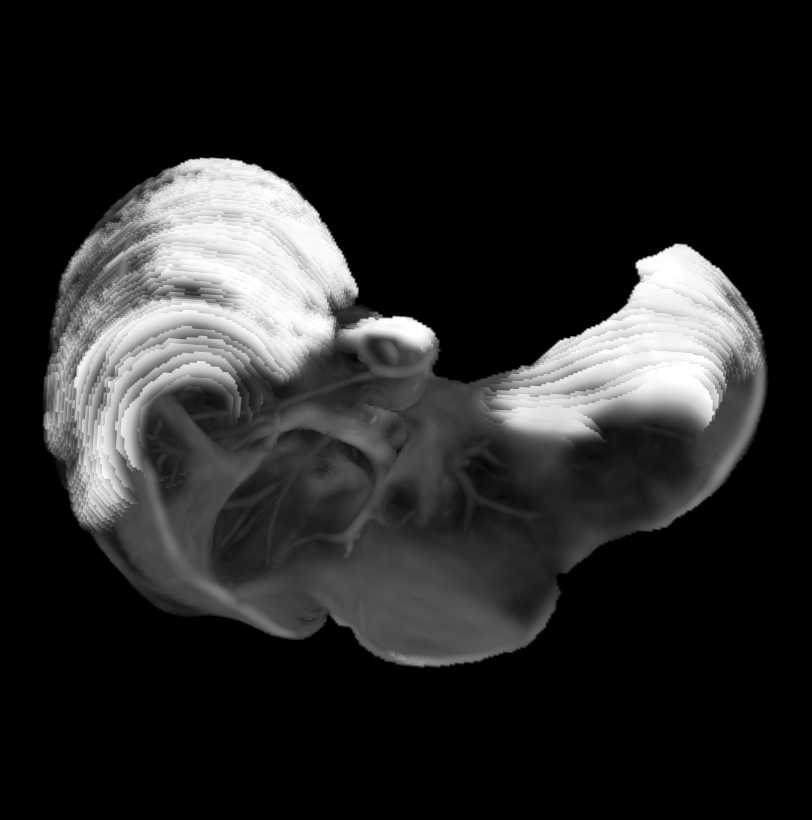
\includegraphics[clip = true, trim  =  10 150 10 150, height=3cm,width=4cm]{Images/Ircad_Meijering.png}
  \caption{Meijering}
  \end{subfigure}
  \begin{subfigure}[t]{0.32\textwidth}
  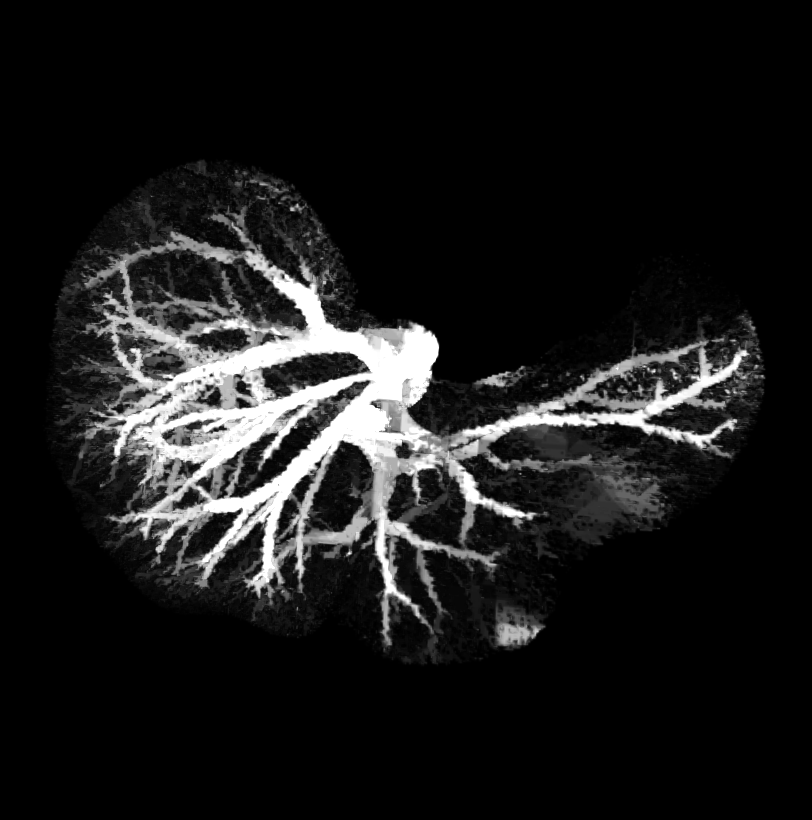
\includegraphics[clip = true, trim  =  10 150 10 150, height=3cm,width=4cm]{Images/Ircad_RORPO.png}
  \caption{RORPO}
  \end{subfigure}
  \begin{subfigure}[t]{0.32\textwidth}
  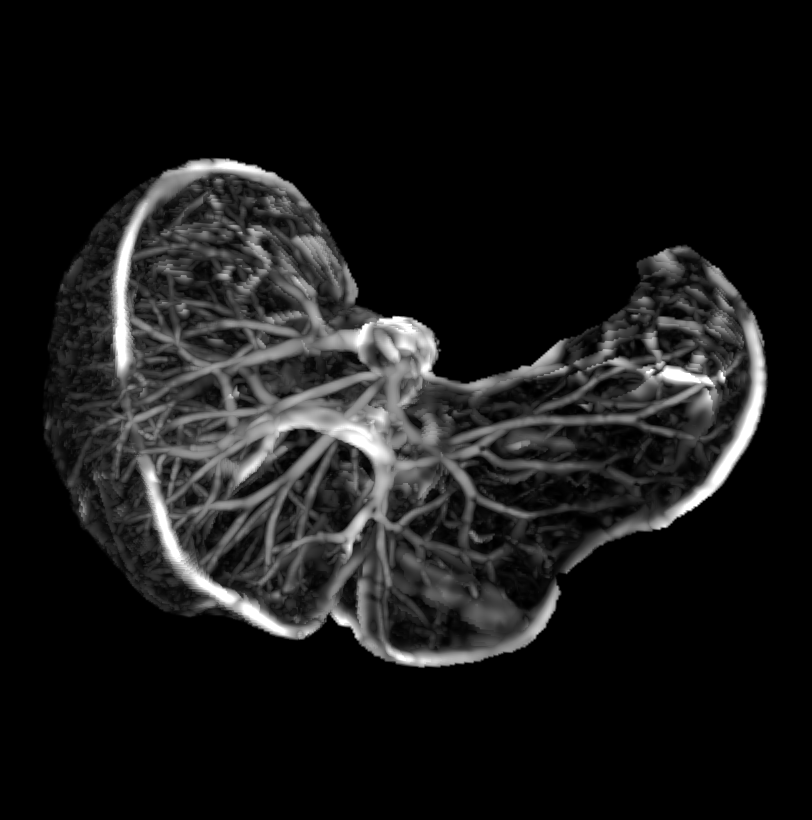
\includegraphics[clip = true, trim  =  10 150 10 150, height=3cm,width=4cm]{Images/Ircad_Sato.png}
  \caption{Sato}
  \end{subfigure}
  \begin{subfigure}[t]{0.32\textwidth}
  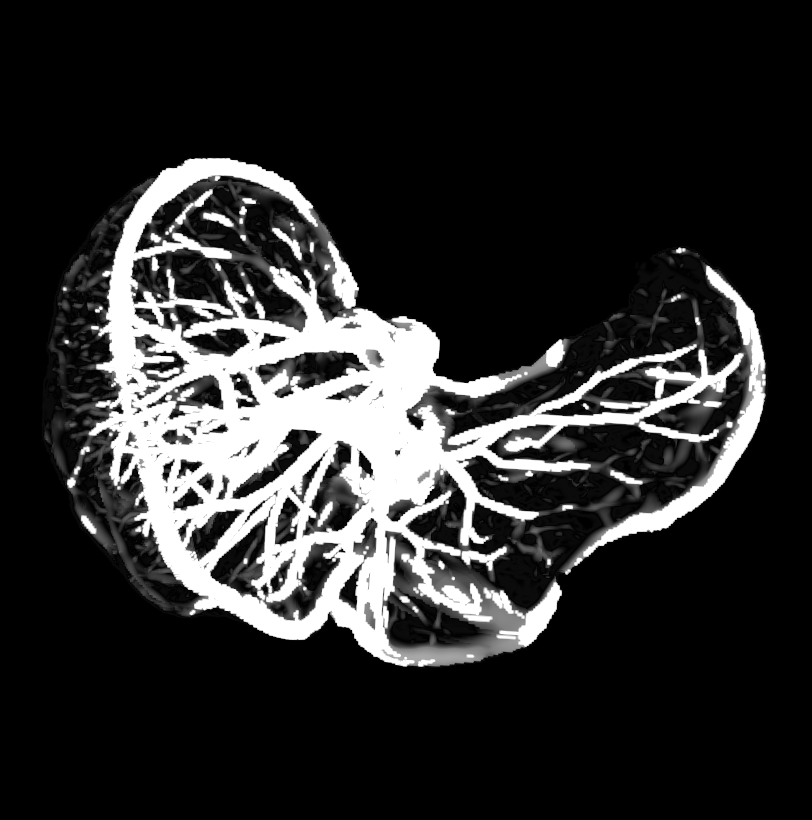
\includegraphics[clip = true, trim  =  10 150 10 150, height=3cm,width=4cm]{Images/Ircad_Zhang.png}
  \caption{Zhang}
  \end{subfigure}
  \centering
  \caption{Illustration des résultats de filtrage optimisé pour l'Ircad.}
  \label{fig:qualitative results Ircad}
  \end{figure}

\paragraph{Bullitt}
\begin{table}[!ht]
  \begin{center}
      \caption{Résultats quantitatifs (moyenne $\pm$ écart-type) dans le masque global \maskglobal sur le jeu de données de Bullitt.}
      \label{tab:quantitative results Bullit}
  \begin{tabular}{lccc}
      \hline
          & MCC & Dice & PSNR \\ 
      \hline
      Témoin	  & $ 0.396 \pm 0.049 $ & $ 0.340 \pm 0.061 $ & $ 20.275 \pm	0.732 $ \\ 
      Frangi	    & $ 0.474 \pm 0.027 $ & $ 0.481 \pm 0.026 $ & $ 21.768 \pm	0.510 $ \\ 
      Jerman	    & $ 0.432 \pm 0.030 $ & $ 0.438 \pm 0.029 $ & $ 19.723 \pm	1.051 $ \\ 
      Meijering	  & $ 0.349 \pm 0.040 $ & $ 0.354 \pm 0.043 $ & $ 21.905 \pm	0.463 $ \\ 
      OOF	        & $ 0.417 \pm 0.029 $ & $ 0.424 \pm 0.030 $ & $ 21.875 \pm	0.491 $ \\ 
      RORPO	      & $ \tbf{0.543} \pm 0.021 $ & $ \tbf{0.540} \pm 0.023 $ & $ \tbf{21.909} \pm	0.497 $ \\ 
      Sato	      & $ 0.475 \pm 0.026 $ & $ 0.473 \pm 0.028 $ & $ 21.799 \pm	0.466 $ \\ 
      Zhang	      & $ 0.423 \pm 0.037 $ & $ 0.431 \pm 0.037 $ & $ 21.261 \pm	0.847 $ \\ 

      \hline
  \end{tabular} 
\end{center}
\end{table}

Qualitativement (Fig. \ref{fig:qualitative results VascuSynth}), RORPO semble le mieux rehausser les vaisseaux avec peu de bruit. Cependant, les vaisseaux faiblement contrastés présentent des déconnexions irrégulières typiques des filtres anti-extensifs. Quelques méthodes rehaussent le bruit dans les tissus du cerveau plus que d'autres telles que Jerman, Sato, Meijering et OOF. Cependant, Jerman et Sato présentent des profils de vaisseaux bien plus contrastés que le bruit. Le diamètre des vaisseaux est surestimé par Jerman, Zhang, Meijering et dans une moindre mesure par OOF. Cela amène à la fusion de vaisseaux adjacents (voir Fig. \ref{fig:bifurcation_Bullitt}). Le rehaussement de Zhang est irrégulier avec certains vaisseaux très contrastés et d'autres plus faiblement. Cet effet est provoqué par la K-moyenne qui introduit un rehaussement dépendant de la classe associée aux voxels.

Nous attirons l'attention du lecteur sur le fait que nous n'avons pas observé d'artefacts liés au bord sur ce jeu de données puisque nous avons érodé le masque du cerveau de manière à exclure les veines non labellisées qui auraient biaisé nos métriques. 

Quantitativement, RORPO offre de meilleurs résultats par rapport aux autres filtres (MCC=$0.543$). Sato (MCC=$0.475$) et Frangi (MCC=$0.474$) arrivent respectivement en seconde et troisième position. Bien que présentant des MCC proches, le rappel de Frangi est meilleur que celui de Sato  ($0.469$ et $0.399$) mais avec un plus faible taux de précision ($0.498$ vs. $0.585$). Jerman (MCC=$0.432$), Zhang (MCC=$0.424$) et OOF (MCC=$0.417$) présentent des résultats supérieurs au témoin (MCC=$0.396$) tandis que Meijering produit un fort taux de faux positifs qui pénalise le MCC ($0.349$).
\begin{figure}[!ht]
  \captionsetup[subfigure]{justification=centering}
  \begin{subfigure}[t]{0.32\textwidth}
  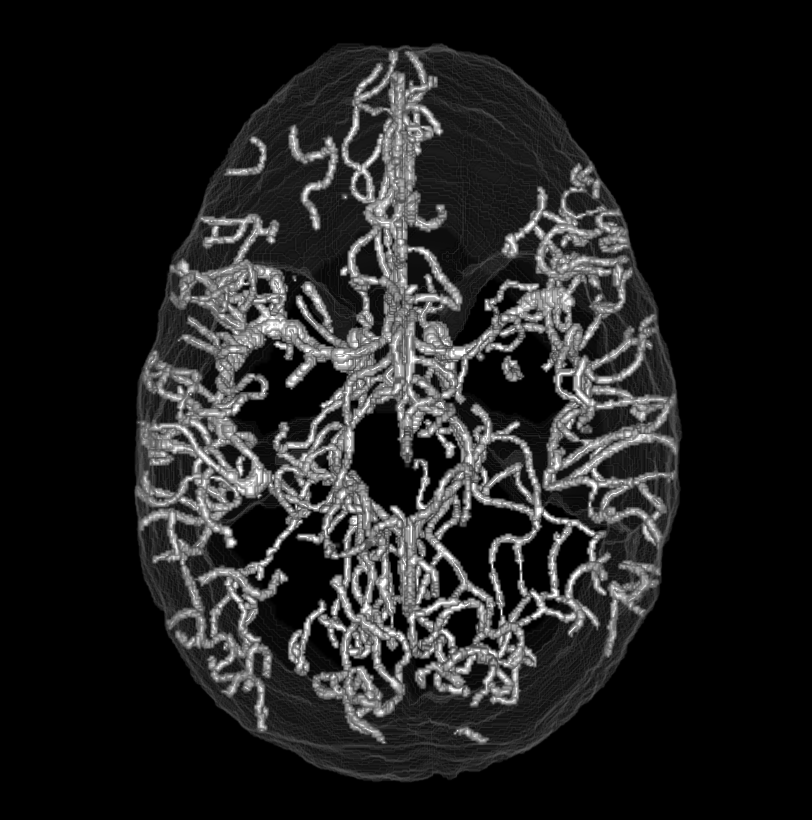
\includegraphics[clip = true, trim = 90 20 90 20, height=4cm,width=3.9cm]{Images/Bullitt_GT.png}
  \caption{Vérité terrain}
\end{subfigure}
  \begin{subfigure}[t]{0.32\textwidth}
  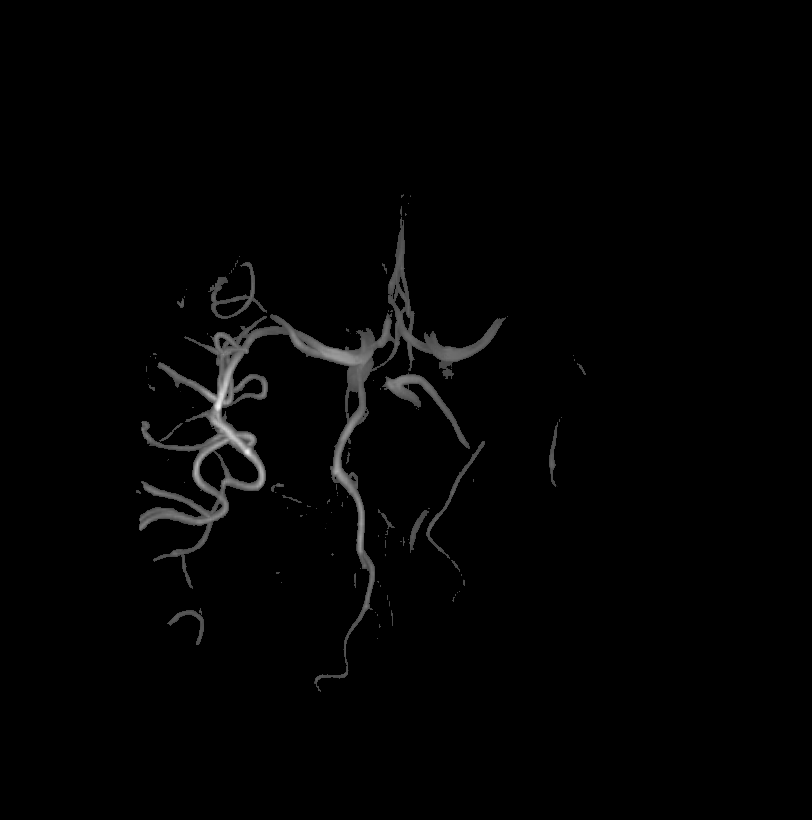
\includegraphics[clip = true, trim = 90 20 90 20, height=4cm,width=3.9cm]{Images/Bullitt_Baseline.png}
  \caption{Témoin}
  \end{subfigure}
  \begin{subfigure}[t]{0.32\textwidth}
  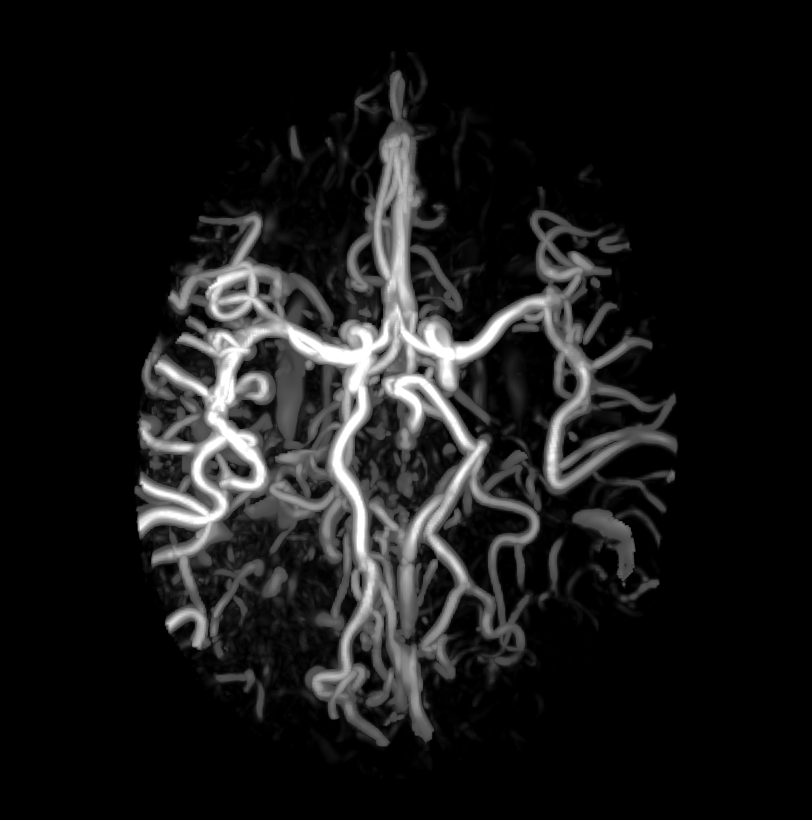
\includegraphics[clip = true, trim = 90 20 90 20, height=4cm,width=3.9cm]{Images/Bullitt_Frangi.png}
  \caption{Frangi}
  \end{subfigure}
  \begin{subfigure}[t]{0.32\textwidth}
  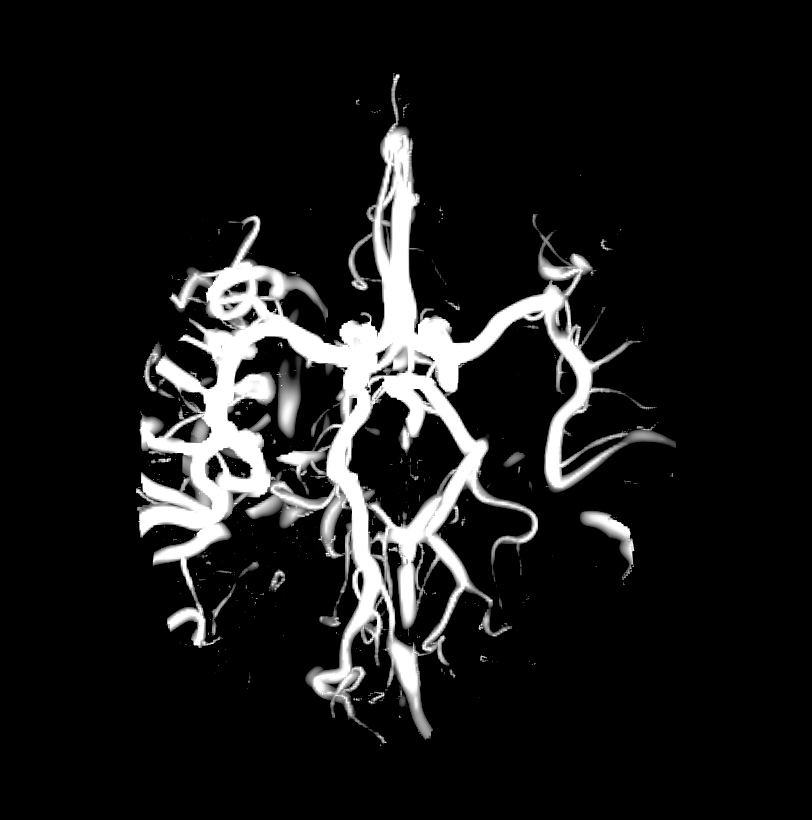
\includegraphics[clip = true, trim = 90 20 90 20, height=4cm,width=3.9cm]{Images/Bullitt_Jerman.png}
  \caption{Jerman}
  \end{subfigure}
  \begin{subfigure}[t]{0.32\textwidth}
  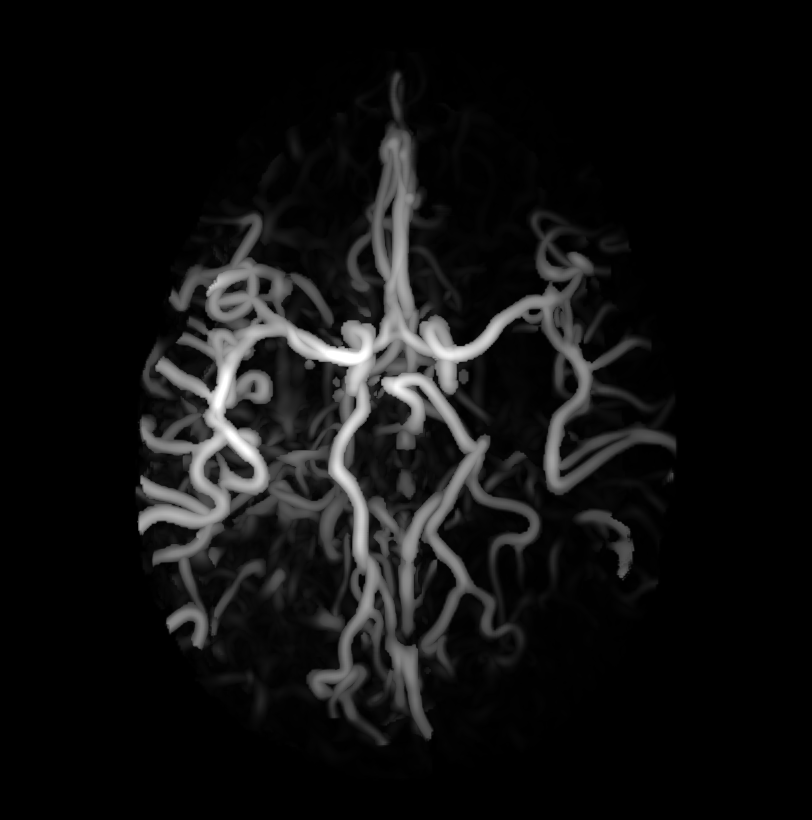
\includegraphics[clip = true, trim = 90 20 90 20, height=4cm,width=3.9cm]{Images/Bullitt_OOF_GM.png}
  \caption{OOF}
  \end{subfigure}
  \begin{subfigure}[t]{0.32\textwidth}
  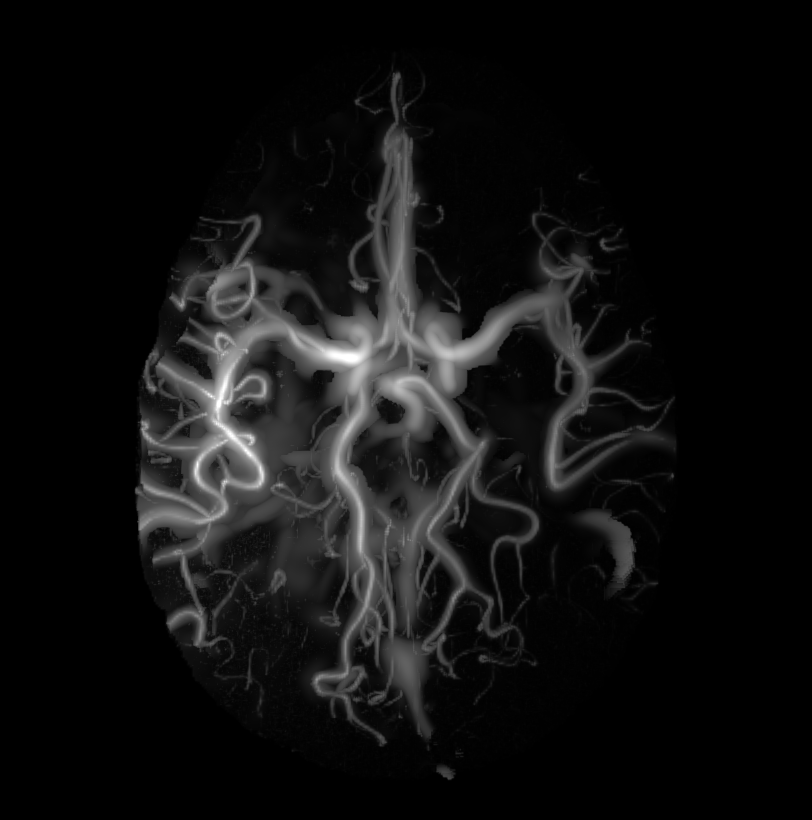
\includegraphics[clip = true, trim = 90 20 90 20, height=4cm,width=3.9cm]{Images/Bullitt_Meijering.png}
  \caption{Meijering}
  \end{subfigure}
  \begin{subfigure}[t]{0.32\textwidth}
  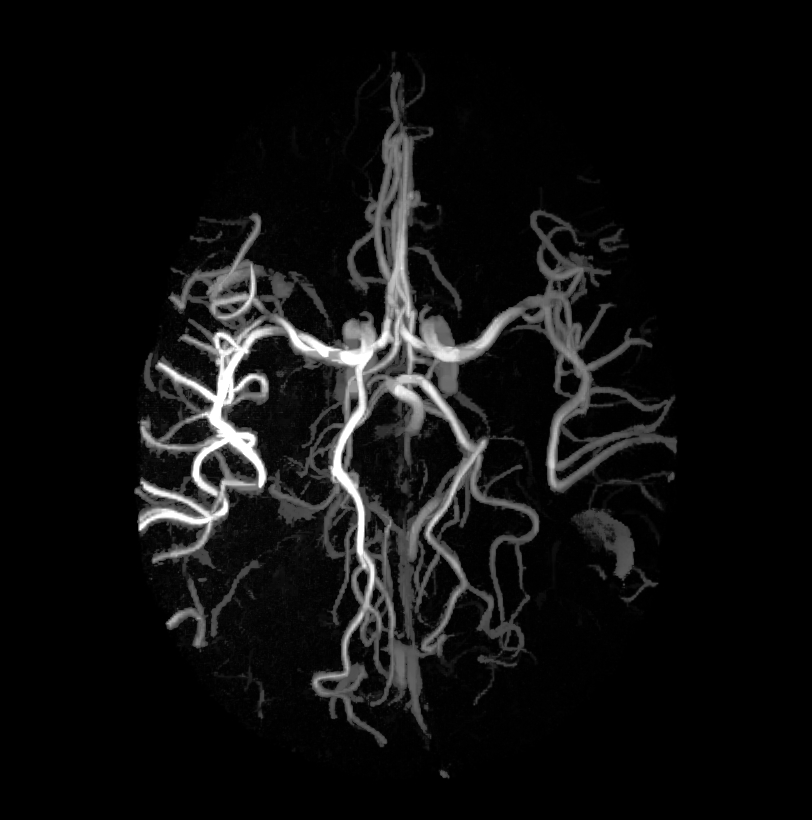
\includegraphics[clip = true, trim = 90 20 90 20, height=4cm,width=3.9cm]{Images/Bullitt_RORPO.png}
  \caption{RORPO}
  \end{subfigure}
  \begin{subfigure}[t]{0.32\textwidth}
  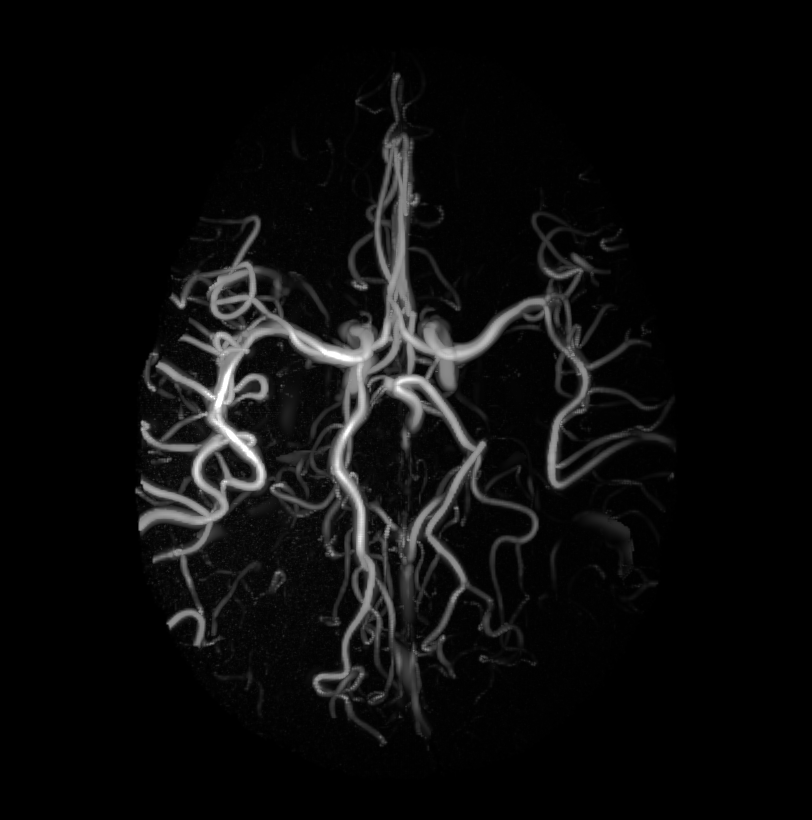
\includegraphics[clip = true, trim = 90 20 90 20, height=4cm,width=3.9cm]{Images/Bullitt_Sato.png}
  \caption{Sato}
  \end{subfigure}
  \begin{subfigure}[t]{0.32\textwidth}
  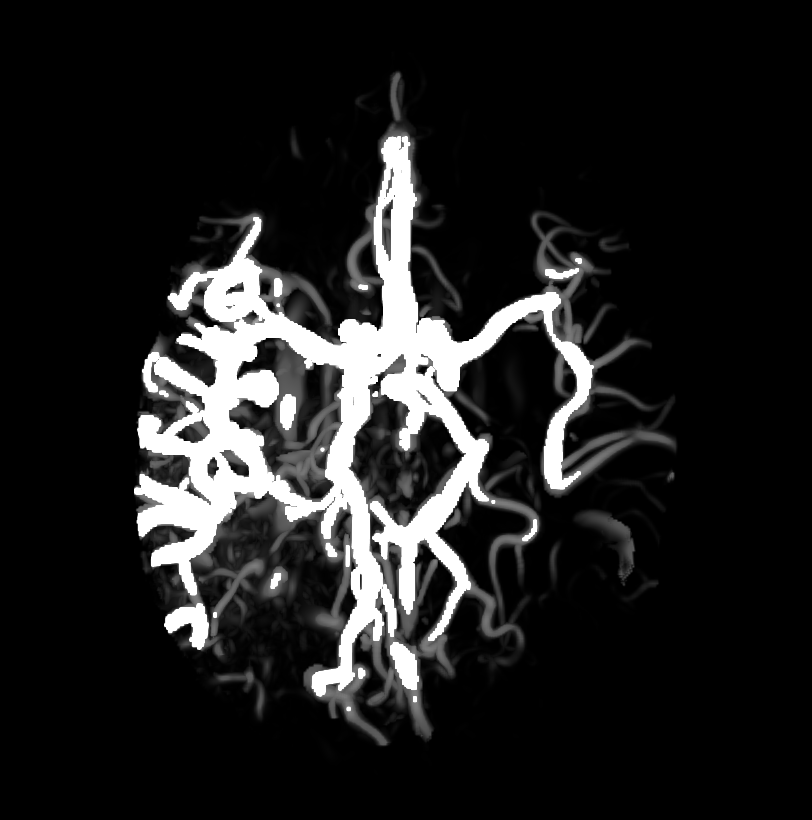
\includegraphics[clip = true, trim = 90 20 90 20, height=4cm,width=3.9cm]{Images/Bullitt_Zhang.png}
  \caption{Zhang}
  \end{subfigure}
  \centering
  \caption{Illustration des résultats de filtrage optimisé pour Bullitt.
  Dans l'ordre de lecture vérités terrains, suivies du témoin, Frangi, Jerman, OOF, Meijering, RORPO, Sato et Zhang.}
  \label{fig:qualitative results VascuSynth}
\end{figure}

\paragraph{VascuSynth}
\begin{table}[!ht]
    \begin{center}
    \caption{Résultats quantitatifs (moyenne $\pm$ écart-type) dans le masque global \maskglobal sur les jeux de données de VascuSynth.}
    \label{Table:quantitative results Vascusynth}
    \resizebox{\textwidth}{!}{
    \begin{tabular}{l|ccc|ccc|ccc}
    \hline
          & \multicolumn{3}{c|}{MCC} & \multicolumn{3}{c|}{Dice} & \multicolumn{3}{c}{PSNR} \\
          & $\sigma = 2$ & $\sigma = 4$ & $\sigma = 6$ & $\sigma = 2$ & $\sigma = 4$ & $\sigma = 6$ & $\sigma = 2$ & $\sigma = 4$ & $\sigma = 6$\\
         \hline
         Témoin	    & $ 0.184 \pm 0.136 $  & $ 0.143 \pm 0.116 $ & $ 0.106 \pm	0.089 $ & $	0.162 \pm 0.134 $ & $ 0.122 \pm 0.114 $ & $	0.089 \pm  0.087 $ & $  9.411 \pm   0.231 $ & $  9.397  \pm 0.230 $ & $  9.374  \pm	0.229 $ \\
         Frangi	    & $ \tbf{0.634} \pm 0.051 $  & $ 0.577 \pm 0.070 $ & $ 0.500 \pm	0.081 $ & $	\tbf{0.621} \pm 0.049 $ & $ 0.572 \pm 0.074 $ & $	0.485 \pm  0.091 $ & $ 26.274 \pm 	2.813 $ & $\tbf{26.496}	\pm 2.872 $	& $ \tbf{26.692}	\pm 2.856 $ \\
         Jerman	    & $ 0.611 \pm 0.064 $  & $ 0.565 \pm 0.049 $ & $ 0.501 \pm	0.048 $ & $	0.603 \pm 0.065 $ & $ 0.549 \pm 0.046 $ & $	0.464 \pm  0.048 $ & $ \tbf{26.774} \pm 	1.296 $ & $	21.758	\pm 0.399 $	& $ 21.831	\pm 0.489 $ \\
         OOF	      & $ 0.627 \pm 0.061 $  & $ 0.496 \pm 0.065 $ & $ 0.449 \pm	0.069 $ & $	0.530 \pm 0.060 $ & $ 0.476 \pm 0.063 $ & $	0.419 \pm  0.067 $ & $ 26.324 \pm 	1.802 $ & $	24.594	\pm 1.329 $	& $ 22.983	\pm 1.072 $ \\
         Meijering	& $ 0.538 \pm 0.061 $  & $ \tbf{0.603} \pm 0.059 $ & $ \tbf{0.565} \pm	0.060 $ & $	0.619 \pm 0.064 $ & $ \tbf{0.599} \pm 0.061 $ & $	\tbf{0.564} \pm  0.059 $ & $ 26.586 \pm 	2.331 $ & $	25.902	\pm 1.889 $	& $ 24.821	\pm 1.395 $ \\
         RORPO	    & $ 0.587 \pm 0.155 $  & $ 0.517 \pm 0.119 $ & $ 0.366 \pm	0.123 $ & $	0.554 \pm 0.157 $ & $ 0.476 \pm 0.117 $ & $	0.325 \pm  0.113 $ & $ 23.236 \pm 	2.472 $ & $	20.672	\pm 1.689 $	& $ 18.372	\pm 1.571 $ \\
         Sato	      & $ 0.618 \pm 0.046 $  & $ 0.559 \pm 0.058 $ & $ 0.488 \pm	0.052 $ & $	0.596 \pm 0.044 $ & $ 0.548 \pm 0.058 $ & $	0.464 \pm  0.050 $ & $ 26.602 \pm 	2.539 $ & $	26.241	\pm 1.803 $	& $ 24.801	\pm 1.285 $ \\
         Zhang	    & $ 0.553 \pm 0.052 $  & $ 0.523 \pm 0.051 $ & $ 0.481 \pm	0.065 $ & $	0.531 \pm 0.051 $ & $ 0.498 \pm 0.049 $ & $	0.474 \pm  0.067 $ & $ 26.221 \pm 	2.805 $ & $	26.360	\pm 2.826 $	& $ 26.543	\pm 2.845 $ \\
   
    \end{tabular} }
    \end{center}
\end{table}
Qualitativement (Fig. \ref{fig:qualitative results VascuSynth}), Meijering, Sato et Jerman produisent les meilleurs résultats. Cependant, Meijering a tendance à rehausser le bruit au voisinage des vaisseaux, donnant à leur contour un aspect irrégulier. Jerman a un rehaussement des vaisseaux de bonne qualité, mais rehausse aussi une partie significative du bruit. Frangi, Zhang et Sato semblent être les meilleures méthodes pour filtrer le bruit ricien. 

Ce jeu de données montre une certaine sensibilité de RORPO au bruit. Plus le bruit augmente et plus les artefacts sont rehaussés. Ce comportement était en partie attendu puisque nous n'avons pas utilisé le paramètre de dilatation de RORPO (qui gère les déconnexions liées au bruit) en le laissant à 0. Ce choix a été motivé par le fait que ce paramètre ne peut pas être optimisé séparément des paramètres d'échelle. Toutefois, dans des applications réelles avec un fort niveau de bruit, l'étude de ce paramètre est indispensable. \newV{On peut aussi noter que comme les autres filtres, RORPO rehausse une partie des blobs gaussiens de forte intensité. Un cas particulier du rehaussement de blob, propre à RORPO, se produit lorsqu'un blob est en contact avec un vaisseau. Dans ce cas, une partie des chemins participant au rehaussement des structures tubulaires peuvent traverser et rehausser les blobs. Ce comportement est par exemple visible lorsqu'un blob gaussien touche l'extrémité d'un vaisseau.}

Comme le jeu de données VascuSynth ne présente pas de bords d'organes où d'artefacts similaires, l'éventualité d'un faux rehaussement lié à ces artefacts est limitée comparativement aux jeux de données réels, excepté pour OOF qui rehausse les bordures de l'image assimilées à des plans. La mesure utilisée pour OOF distingue en effet mal les structures planaires des structures tubulaires. Une autre mesure de tubularité telle que la mesure de Frangi pourrait être utilisée pour éviter ce problème. De manière générale, quand le bruit n'est pas bien filtré, les filtres de rehaussement ont tendance à introduire de fausses structures tubulaires non présentes dans l'image d'origine (Fig. \ref{fig:noisy_tubes}).
\begin{figure}[!ht]
  \centering
  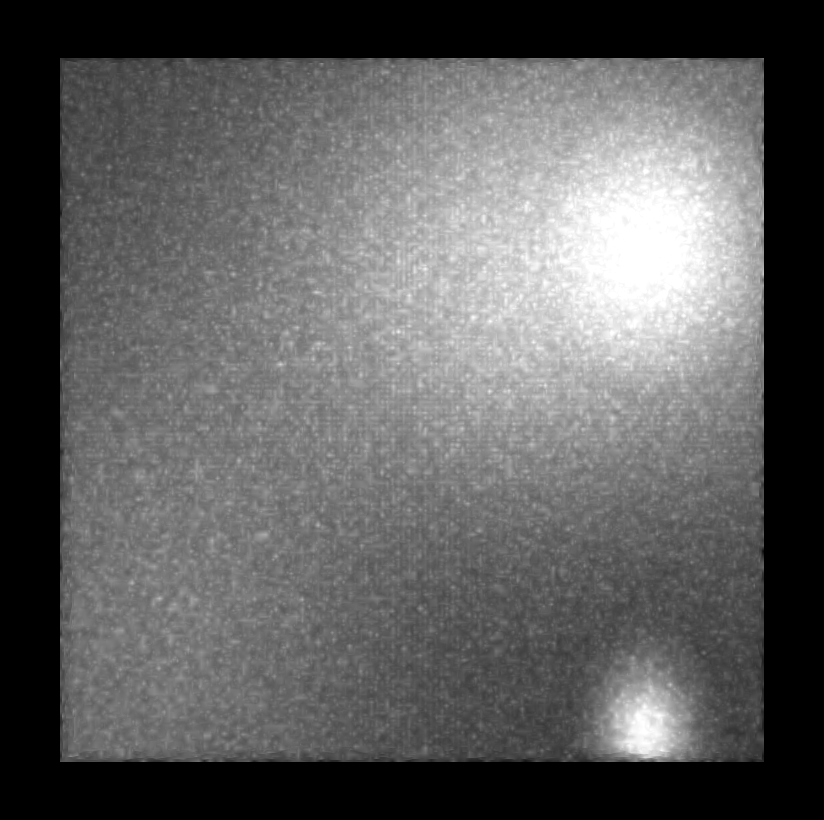
\includegraphics[height=4cm]{Images/vascu_noise.png}
  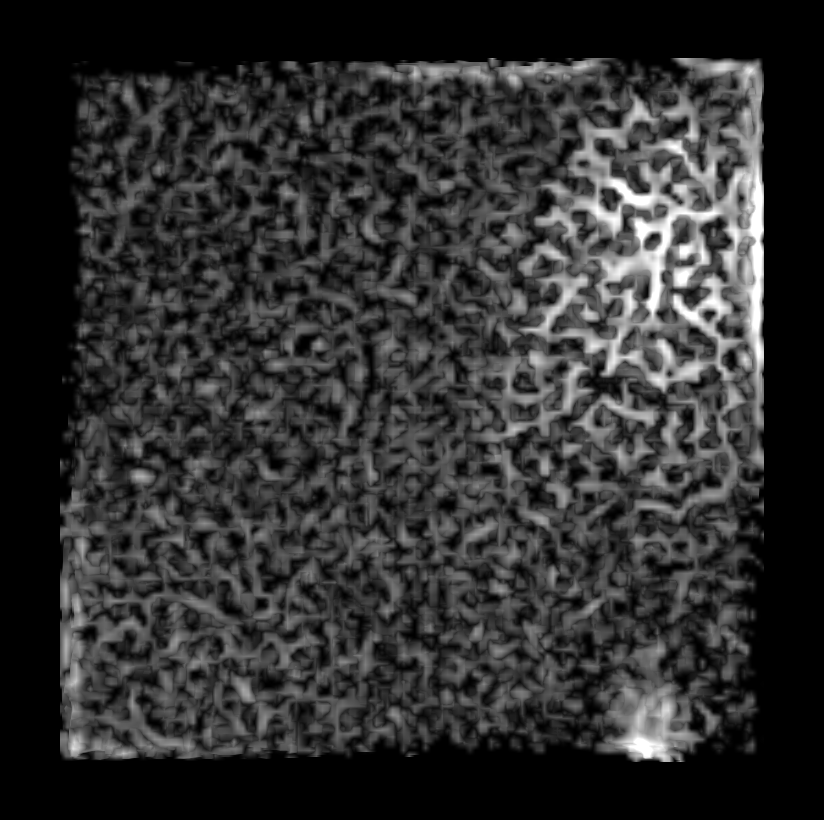
\includegraphics[height=4cm]{Images/vascu_noise_OOF.png}
  \caption{Bruit de fond de Vascusynth $\sigma=4$ et bruit de fond après filtrage par OOF. Après filtrage, le bruit forme des structures tubulaires de faible intensité pour la plupart des filtres matriciels.}
  \label{fig:noisy_tubes}
\end{figure}

Quantitativement, Frangi donne les meilleurs résultats pour $\sigma=2$ avec un MCC de $0.634$. Meijering  atteint un MCC de $0.603$ pour $\sigma=4$ et $0.565$ pour $\sigma=6$. Ces bonnes performances de Meijering peuvent s'expliquer par le fait que la géométrie des vaisseaux de VascuSynth corresponde aux hypothèses du modèle de Meijering (vaisseaux droits et de rayon constant). Sato obtient le troisième meilleur résultat pour le niveau de bruit $\sigma=2$ (MCC=$0.618$) tandis que Jerman présente de meilleurs résultats pour des niveaux de bruits supérieurs (MCC = $0.565$ pour $\sigma=4$ et MCC=$0.501$ pour $\sigma = 6$). Peu importe les cas, les deux filtres donnent des résultats similaires, puisque leur sensibilité est proche, indépendamment du niveau de bruit. La différence entre les deux filtres s'explique au niveau de la précision : pour des niveaux de bruit élevés (e.g. $\sigma=4$), Jerman présente une plus grande précision (MCC = $0.717$ vs. $0.661$) tandis que Sato présente une précision supérieure pour les faibles niveaux de bruit (MCC = $0.810$ vs. $0.689$). En général, Frangi est la méthode la plus robuste au bruit pour des niveaux de bruit élevés avec un PSNR de $26.496$ et $26.692$ pour $\sigma=4$ et $\sigma=6$, respectivement. Les résultats du témoin sont très mauvais à cause de la présence d'artefacts de haute intensité et d'un fond non homogène dans les données de VascuSynth. Ce comportement est une motivation supplémentaire pour l'usage de filtres de rehaussement pour des applications avec un contexte similaire. Globalement, RORPO produit les moins bons résultats sur VascuSynth alors que Zhang reste relativement stable, peu importe le niveau de bruit choisi.
\begin{figure}[!ht]
  \captionsetup[subfigure]{justification=centering}
  \begin{subfigure}[t]{0.32\textwidth}
    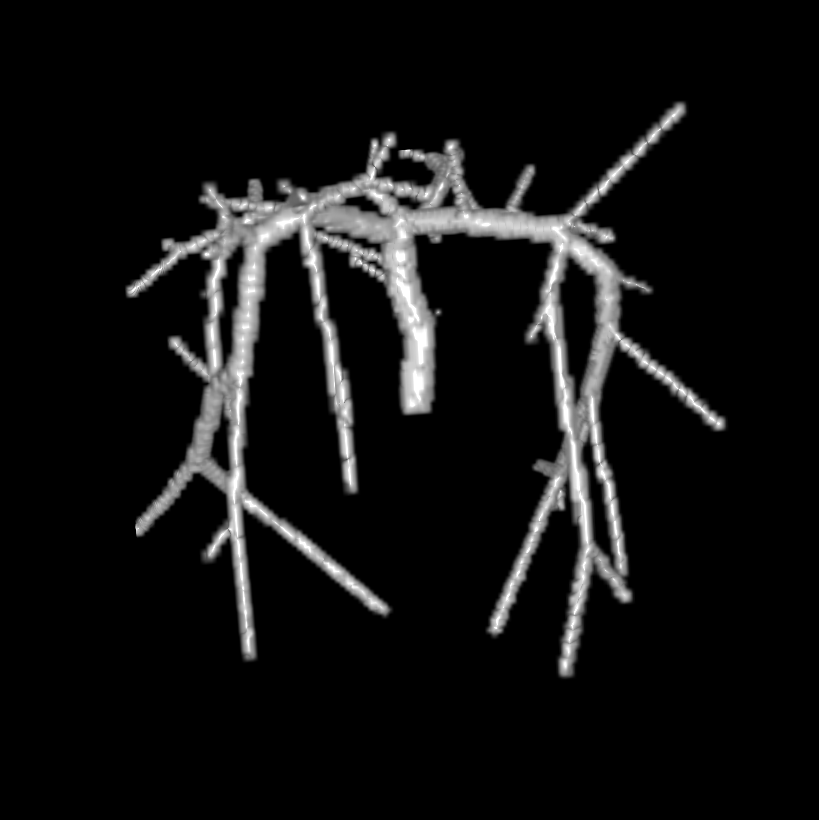
\includegraphics[clip = true, trim = 80 80 80 80,width=\textwidth]{Images/Vascu_4_GT.png}
    \caption{Vérité terrain}  
  \end{subfigure}
  \begin{subfigure}[t]{0.32\textwidth}
    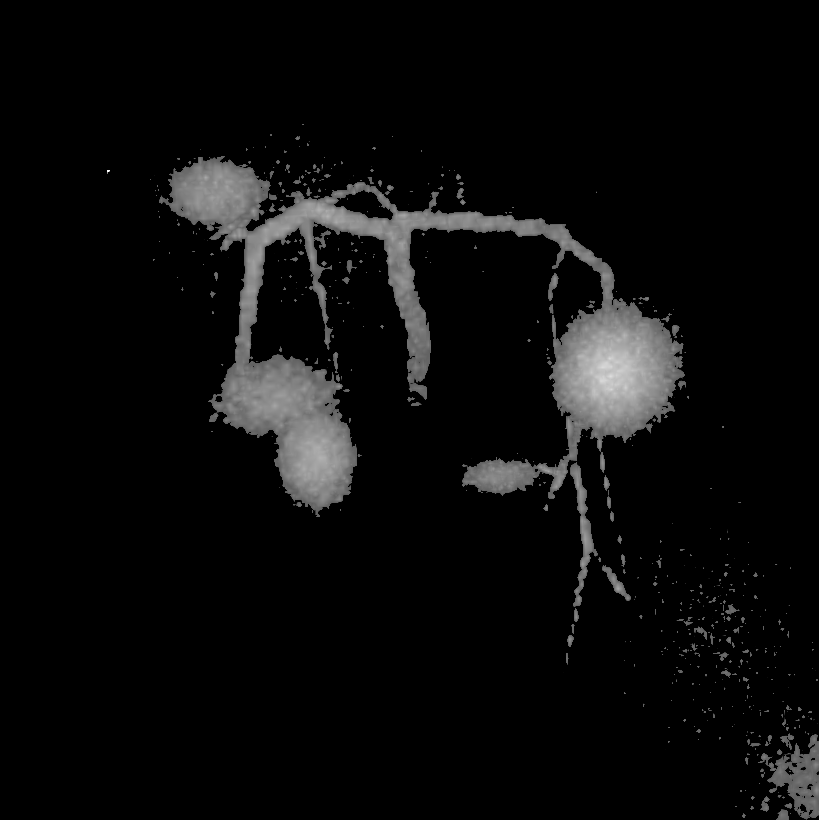
\includegraphics[clip = true, trim = 80 80 80 80,width=\textwidth]{Images/Vascu_4_Baseline.png}
    \caption{Témoin}
  \end{subfigure}
  \begin{subfigure}[t]{0.32\textwidth}
    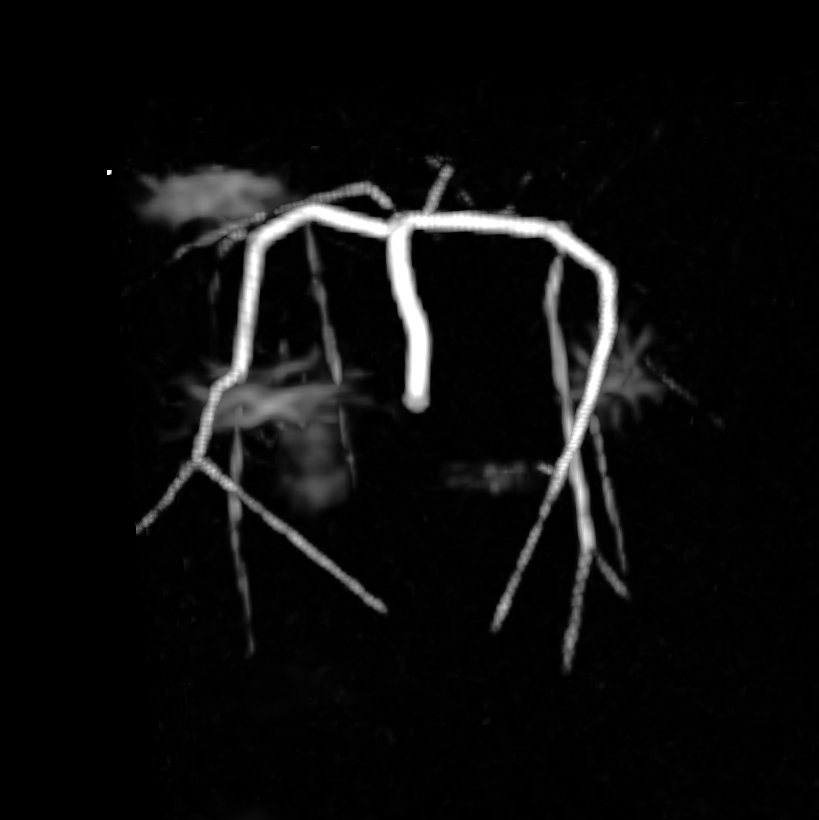
\includegraphics[clip = true, trim = 80 80 80 80,width=\textwidth]{Images/Vascu_4_Frangi.png}  
    \caption{Frangi}
  \end{subfigure}
  \begin{subfigure}[t]{0.32\textwidth}
    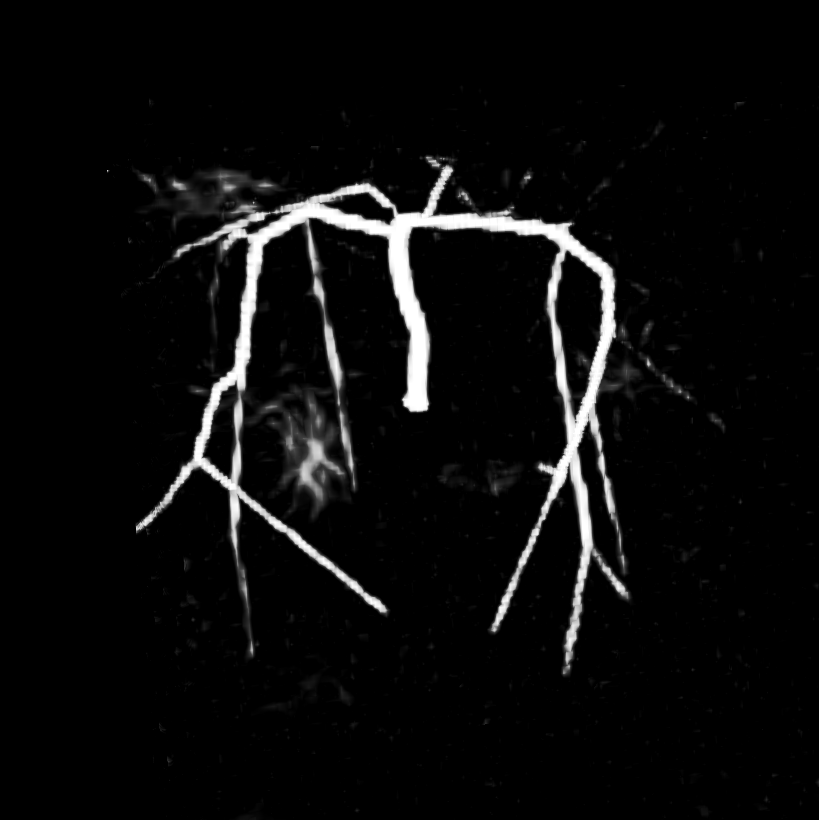
\includegraphics[clip = true, trim = 80 80 80 80,width=\textwidth]{Images/Vascu_4_Jerman.png}
    \caption{Jerman}
  \end{subfigure}
  \begin{subfigure}[t]{0.32\textwidth}
    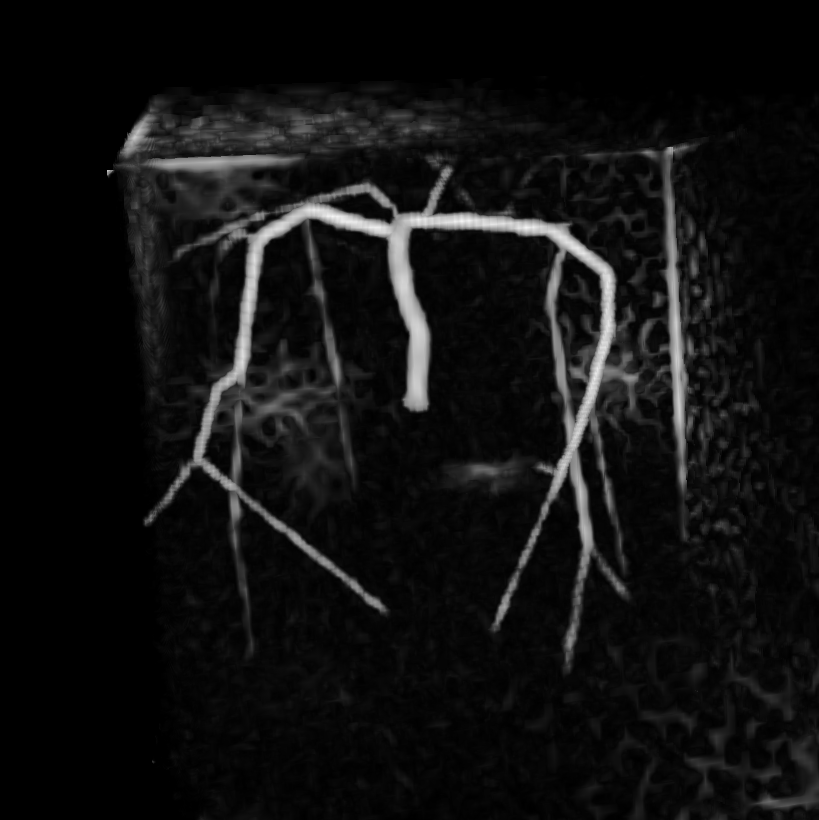
\includegraphics[clip = true, trim = 80 80 80 80,width=\textwidth]{Images/Vascu_4_OOF_GM.png}
    \caption{OOF}
  \end{subfigure}
  \begin{subfigure}[t]{0.32\textwidth}
    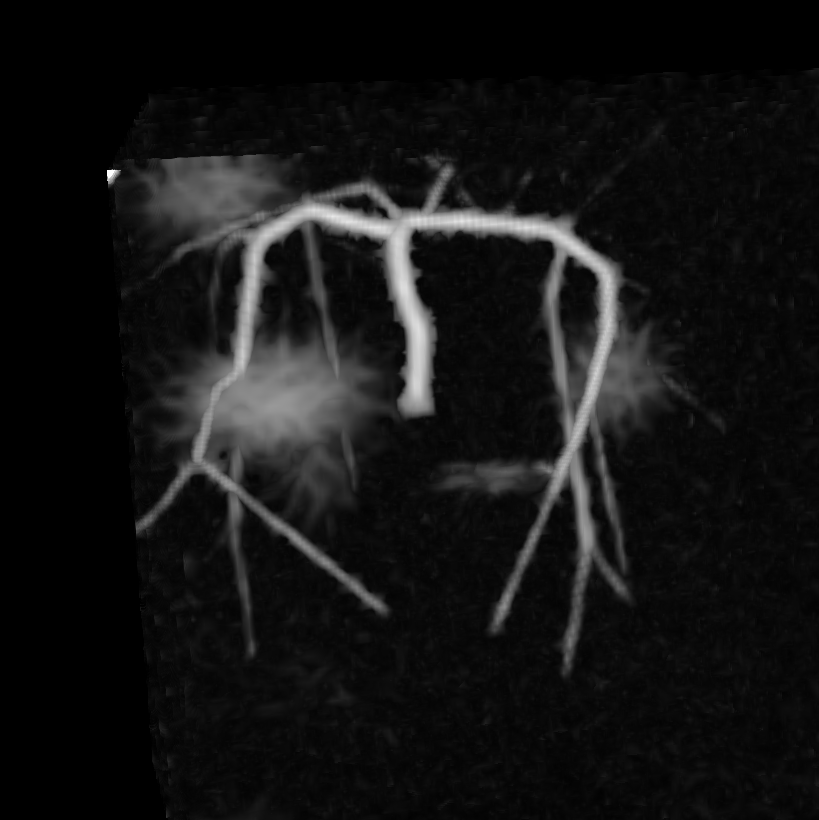
\includegraphics[clip = true, trim = 80 80 80 80,width=\textwidth]{Images/Vascu_4_Meijering.png}
    \caption{Meijering}
  \end{subfigure}
  \begin{subfigure}[t]{0.32\textwidth}
    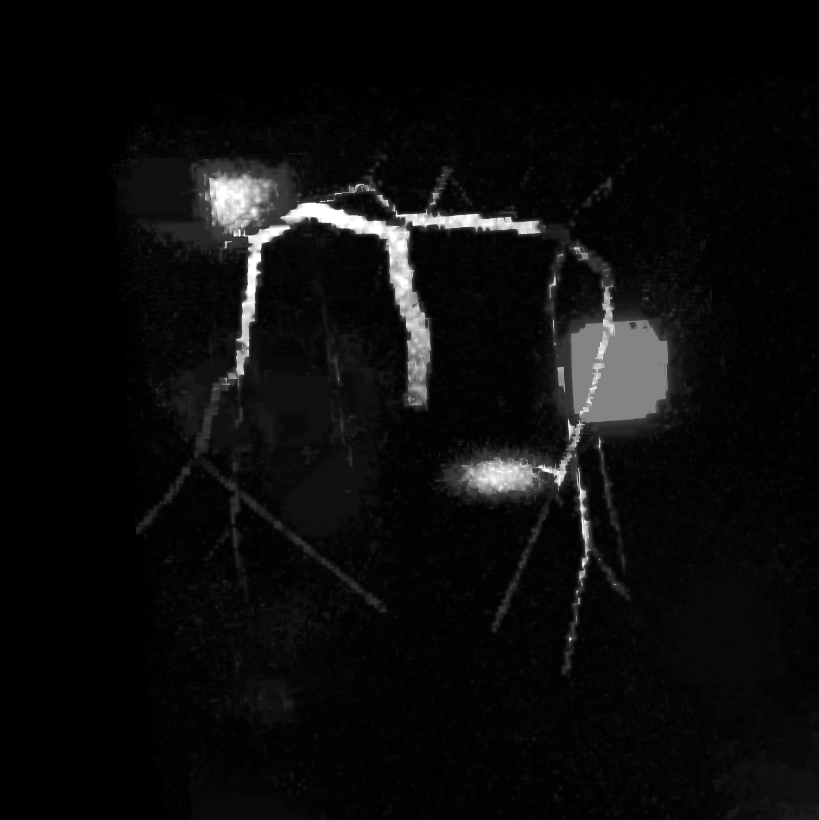
\includegraphics[clip = true, trim = 80 80 80 80,width=\textwidth]{Images/Vascu_4_RORPO.png}
    \caption{RORPO}
  \end{subfigure}
  \begin{subfigure}[t]{0.32\textwidth}
    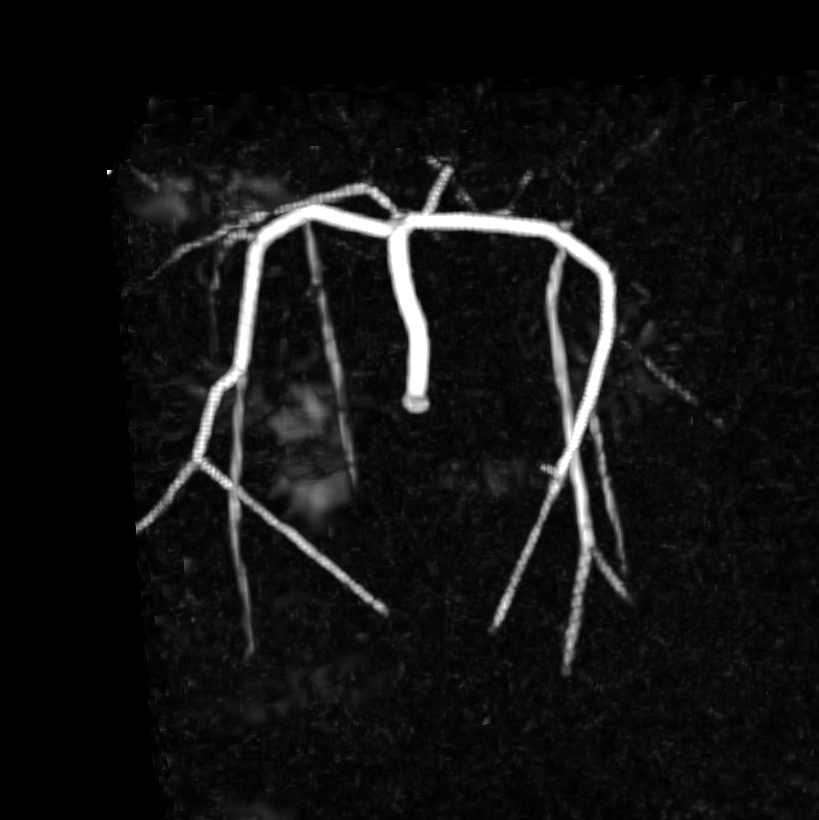
\includegraphics[clip = true, trim = 80 80 80 80,width=\textwidth]{Images/Vascu_4_Sato.png}
    \caption{Sato}
  \end{subfigure}
  \begin{subfigure}[t]{0.32\textwidth}
    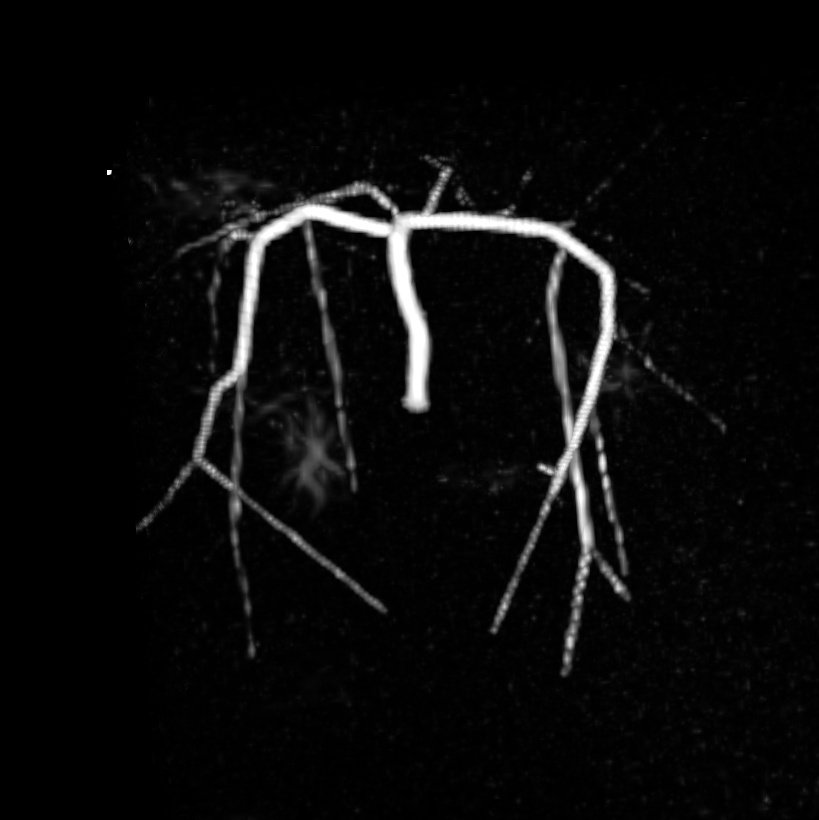
\includegraphics[clip = true, trim = 80 80 80 80,width=\textwidth]{Images/Vascu_4_Zhang.png}
    \caption{Zhang}
  \end{subfigure}
  \centering
  \caption{Illustration des résultats de filtrage optimisé pour VascuSynth $\sigma=4$.}
  \label{fig:qualitative results VascuSynth}
\end{figure}

\subsection{Voisinage des vaisseaux}
Les résultats quantitatifs des sept filtres sont présentés dans les tables \ref{tab:VesselssizeIrcad}--\ref{tab:Vessels size VascuSynth} pour les jeux de données de l'Ircad, Bullitt et VascuSynth.
\paragraph{Ircad}
\begin{table}[!ht]
  \begin{center}
  \caption{Résultats quantitatifs (moyenne $\pm$ écart-type) par catégorie de tailles de vaisseaux pour l'Ircad.}
  \label{tab:VesselssizeIrcad}
  \resizebox{\textwidth}{!}{    
  \begin{tabular}{lccc|ccc}
                \hline
                & \multicolumn{3}{c}{Voisinage (\maskvascular)} & \multicolumn{3}{c}{Larges (\maskvesselLarge)}                                            \\
                \hline
                & MCC  &  Dice & PSNR & MCC  &  Dice  &  PSNR  \\
                Témoin	& $ 0.491 \pm	0.118 $ & $	0.527 \pm 0.110 $ & $ 13.110 \pm 1.795 $ & $ 0.552 \pm 	0.130 $ & $	0.597 \pm 0.136 $ & $ 20.938 \pm 2.637 $ \\
                Frangi  	& $ 0.535 \pm	0.073 $ & $	\tbf{0.581} \pm 0.065 $ & $ 19.989 \pm 1.653 $ & $ \tbf{0.580} \pm 	0.072 $ & $	\tbf{0.627} \pm 0.087 $ & $ 22.189 \pm 1.867 $ \\
                Jerman	  & $ 0.501 \pm	0.054 $ & $	0.521 \pm 0.060 $ & $ \tbf{21.464} \pm 1.757 $ & $ 0.480 \pm 	0.065 $ & $	0.496 \pm 0.083 $ & $ \tbf{24.119} \pm 1.972 $ \\
                Meijering	& $ 0.451 \pm	0.061 $ & $	0.522 \pm 0.049 $ & $ 20.091 \pm 1.646 $ & $ 0.545 \pm 	0.055 $ & $	0.669 \pm 0.044 $ & $ 22.407 \pm 1.850 $ \\
                OOF	      & $ 0.498 \pm	0.063 $ & $	0.556 \pm 0.051 $ & $ 19.912 \pm 1.642 $ & $ 0.513 \pm 	0.060 $ & $	0.574 \pm 0.067 $ & $ 22.056 \pm 1.850 $ \\
                RORPO	    & $ 0.491 \pm	0.066 $ & $	0.501 \pm 0.075 $ & $ 20.463 \pm 1.765 $ & $ 0.491 \pm 	0.069 $ & $	0.504 \pm 0.080 $ & $ 22.580 \pm 1.948 $ \\
                Sato	    & $ 0.508 \pm	0.054 $ & $	0.542 \pm 0.057 $ & $ 19.996 \pm 1.679 $ & $ 0.512 \pm 	0.067 $ & $	0.548 \pm 0.086 $ & $ 22.130 \pm 1.861 $ \\
                Zhang	    & $ \tbf{0.535} \pm	0.064 $ & $	0.551 \pm 0.074 $ & $ 20.940 \pm 1.857 $ & $ 0.541 \pm 	0.078 $ & $	0.561 \pm 0.101 $ & $ 23.199 \pm 2.032 $ \\
      
                \hline
                & \multicolumn{3}{c}{Moyens (\maskvesselMedium)}  & \multicolumn{3}{c}{Petits (\maskvesselSmall)}                                            \\
                \hline
                & MCC  &  Dice & PSNR & MCC  &  Dice  &  PSNR  \\
                Témoin	& $ 0.509 \pm 0.121 $ & $	0.557 \pm 0.117 $ & $ 21.250 \pm 2.989 $ & $ 0.391 \pm	0.103 $ & $	0.424 \pm 0.097 $ & $ 18.687 \pm 2.209 $ \\
                Frangi    & $ 0.619 \pm 0.115 $ & $	0.660 \pm 0.113 $ & $ 27.387 \pm 2.554 $ & $ 0.460 \pm	0.123 $ & $	0.506 \pm 0.118 $ & $ 26.624 \pm 2.232 $ \\
                Jerman    & $ 0.604 \pm 0.095 $ & $	0.622 \pm 0.110 $ & $ \tbf{30.111} \pm 3.155 $ & $ 0.502 \pm	0.093 $ & $	0.525 \pm 0.104 $ & $ \tbf{27.991} \pm 2.120 $ \\
                Meijering & $ 0.542 \pm 0.085 $ & $	0.602 \pm 0.082 $ & $ 27.432 \pm 2.474 $ & $ 0.419 \pm	0.088 $ & $	0.462 \pm 0.077 $ & $ 26.723 \pm 2.187 $ \\
                OOF	      & $ \tbf{0.642} \pm 0.097 $ & $	0.681 \pm 0.097 $ & $ 27.334 \pm 2.467 $ & $ \tbf{0.514} \pm	0.103 $ & $	\tbf{0.559} \pm 0.096 $ & $ 26.692 \pm 2.251 $ \\
                RORPO	    & $ 0.547 \pm 0.102 $ & $	0.573 \pm 0.115 $ & $ 28.138 \pm 2.637 $ & $ 0.417 \pm	0.093 $ & $	0.435 \pm 0.104 $ & $ 27.157 \pm 2.354 $ \\
                Sato	    & $ 0.602 \pm 0.096 $ & $	\tbf{0.629} \pm 0.105 $ & $ 27.437 \pm 2.548 $ & $ 0.488 \pm	0.092 $ & $	0.522 \pm 0.091 $ & $ 26.777 \pm 2.277 $ \\
                Zhang	    & $ 0.602 \pm 0.110 $ & $	0.619 \pm 0.126 $ & $ 28.808 \pm 3.119 $ & $ 0.481 \pm	0.110 $ & $	0.497 \pm 0.124 $ & $ 27.471 \pm 2.311 $ \\        
      \hline
      \end{tabular}

  }
  \end{center}
\end{table}

Tous les filtres hessiens et OOF ont des performances qui augmentent significativement quand ils sont calculés dans \maskvessel, puisque les artefacts éloignés des vaisseaux sont ignorés pour ce masque. Alors que RORPO présentait les meilleurs résultats dans \maskglobal, pour \maskvessel, ce sont Frangi et Zhang qui obtiennent le meilleur MCC (MCC=$0.535$). En étudiant les performances des filtres en fonction de la taille des vaisseaux rehaussés (\maskvesselLarge, \maskvesselMedium, \maskvesselSmall), on observe que Frangi est capable de bien rehausser les vaisseaux larges (MCC=$0.580$) et moyens (MCC= $0.619$), mais ses performances baissent pour les petits vaisseaux (MCC=$0.460$). À l'inverse, OOF et Jerman rehaussent correctement les petits vaisseaux (MCC=$0.514$ et MCC=$0.502$) mais avec des performances réduites sur les gros vaisseaux (MCC=$0.513$ et MCC=$0.480$).   
\paragraph{Bullitt}
\begin{table}[!ht]
  \begin{center}
  \label{tab:Vessels size Bullitt}
  \caption{Résultats quantitatifs (moyenne $\pm$ écart-type) par catégorie de tailles de vaisseaux pour Bullitt.}
  
  \begin{tabular}{lccc}
            \hline
            & \multicolumn{3}{c}{Voisinage (\maskvascular)}                  \\
            \hline
            & MCC & Dice & PSNR  \\
            Témoin	    & $ 0.371 \pm 0.038 $ & $ 0.341 \pm 0.062 $ & $ \tbf{22.291} \pm	0.513 $ \\
            Frangi	      & $ 0.415 \pm 0.028 $ & $ 0.506 \pm 0.026 $ & $ 21.641 \pm	0.517 $ \\
            Jerman	      & $ 0.377 \pm 0.037 $ & $ 0.466 \pm 0.029 $ & $ 21.990 \pm	0.687 $ \\
            Meijering	    & $ 0.288 \pm 0.041 $ & $ 0.412 \pm 0.045 $ & $ 22.076 \pm	0.509 $ \\ 
            OOF	          & $ 0.353 \pm 0.026 $ & $ 0.456 \pm 0.032 $ & $ 21.771 \pm	0.506 $ \\
            RORPO	        & $ \tbf{0.506} \pm 0.022 $ & $ \tbf{0.556} \pm 0.025 $ & $ 21.784 \pm	0.506 $ \\
            Sato	        & $ 0.435 \pm 0.027 $ & $ 0.491 \pm 0.029 $ & $ 21.698 \pm	0.478 $ \\
            Zhang	        & $ 0.348 \pm 0.029 $ & $ 0.460 \pm 0.026 $ & $ 21.430 \pm	0.553 $ \\
      
            \hline
            & \multicolumn{3}{c}{Moyens (\maskvesselMedium)}                         \\
            \hline    
            & MCC & Dice & PSNR  \\
            Témoin	& $ 0.542 \pm 0.129 $ & $ 0.555 \pm 0.163 $ & $ 33.836 \pm	2.891 $ \\
            Frangi	  & $ 0.605 \pm 0.034 $ & $ 0.684 \pm 0.034 $ & $ 33.262 \pm	2.827 $ \\
            Jerman	  & $ 0.580 \pm 0.048 $ & $ 0.660 \pm 0.055 $ & $ \tbf{34.066} \pm	3.226 $ \\
            Meijering	& $ 0.402 \pm 0.054 $ & $ 0.521 \pm 0.067 $ & $ 34.034 \pm	2.820 $ \\
            OOF	      & $ 0.620 \pm 0.049 $ & $ \tbf{0.690} \pm 0.044 $ & $ 33.621 \pm	2.971 $ \\
            RORPO	    & $ \tbf{0.647} \pm 0.047 $ & $ 0.712 \pm 0.047 $ & $ 33.370 \pm	2.882 $ \\
            Sato	    & $ 0.594 \pm 0.064 $ & $ 0.663 \pm 0.088 $ & $ 33.072 \pm	2.928 $ \\
            Zhang	    & $ 0.577 \pm 0.074 $ & $ 0.655 \pm 0.101 $ & $ 33.789 \pm	2.790 $ \\
            \hline
            & \multicolumn{3}{c}{Petits (\maskvesselSmall)}                          \\
            \hline
            & MCC & Dice & PSNR  \\
            Témoin	    & $ 0.358 \pm 0.038 $ & $ 0.315 \pm 0.057 $ & $ \tbf{22.771} \pm	0.591 $ \\
            Frangi	      & $ 0.419 \pm 0.024 $ & $ 0.491 \pm 0.026 $ & $ 22.153 \pm	0.609 $ \\
            Jerman  	    & $ 0.376 \pm 0.031 $ & $ 0.445 \pm 0.030 $ & $ 22.352 \pm	0.863 $ \\
            Meijering	    & $ 0.287 \pm 0.040 $ & $ 0.382 \pm 0.044 $ & $ 22.549 \pm	0.593 $ \\
            OOF	          & $ 0.353 \pm 0.025 $ & $ 0.436 \pm 0.038 $ & $ 22.275 \pm	0.586 $ \\
            RORPO	        & $ \tbf{0.510} \pm 0.023 $ & $ \tbf{0.544} \pm 0.027 $ & $ 22.307 \pm	0.590 $ \\
            Sato	        & $ 0.436 \pm 0.024 $ & $ 0.473 \pm 0.031 $ & $ 22.236 \pm	0.572 $ \\
            Zhang	        & $ 0.349 \pm 0.022 $ & $ 0.440 \pm 0.023 $ & $ 21.861 \pm	0.680 $ \\
  \hline
  \end{tabular}
  \end{center}
\end{table}
Localement, les résultats pour \maskglobal et \maskvessel sont similaires puisque le jeu de données ne contient quasiment pas de structures autres que les vaisseaux. Dans ce contexte, RORPO est toujours le meilleur filtre suivi de Sato et Frangi.
\paragraph{VascuSynth}
\begin{table}[!ht]
  \begin{centering}
  \caption{Résultats quantitatifs (moyenne $\pm$ écart-type) par catégorie de tailles de vaisseaux pour VascuSynth ($\sigma=2$).}
  \label{tab:Vessels size VascuSynth}
  \resizebox{\textwidth}{!}{
  \begin{tabular}{lccc|ccc}
            \hline
            & \multicolumn{3}{c}{Voisinage (\maskvascular)}  & \multicolumn{3}{c}{Larges (\maskvesselLarge)}                           \\
            \hline
            & MCC   & Dice & PSNR & MCC & Dice & PSNR  \\
            Témoin	    & $ 0.392 \pm 0.145 $ & $ 0.340 \pm	0.172 $ & $	25.198 \pm	3.109 $ & $ 0.515 \pm 0.293 $ & $ 0.491 \pm 0.307 $ & $ 30.738 \pm 1.278 $ \\
            Frangi	      & $ 0.700 \pm 0.037 $ & $ 0.688 \pm	0.044 $ & $	26.275 \pm	2.814 $ & $ 0.757 \pm 0.022 $ & $ 0.747 \pm 0.025 $ & $ 32.939 \pm 0.934 $ \\
            Jerman	      & $ 0.710 \pm 0.055 $ & $ 0.702 \pm	0.067 $ & $	\tbf{29.880} \pm	3.007 $ & $ 0.735 \pm 0.027 $ & $ 0.722 \pm 0.031 $ & $ 36.312 \pm 0.973 $ \\
            Meijering	    & $ \tbf{0.725} \pm 0.034 $ & $ \tbf{0.753} \pm	0.035 $ & $	27.305 \pm	2.969 $ & $ \tbf{0.818} \pm 0.028 $ & $ \tbf{0.834} \pm 0.028 $ & $ 34.217 \pm 0.978 $ \\
            OOF	          & $ 0.648 \pm 0.043 $ & $ 0.624 \pm	0.053 $ & $	28.275 \pm	2.968 $ & $ 0.714 \pm 0.025 $ & $ 0.696 \pm 0.029 $ & $ 35.068 \pm 0.980 $ \\
            RORPO	        & $ 0.639 \pm 0.082 $ & $ 0.619 \pm	0.096 $ & $	29.406 \pm	3.407 $ & $ 0.713 \pm 0.165 $ & $ 0.694 \pm 0.197 $ & $ \tbf{37.049} \pm 1.574 $ \\
            Sato	        & $ 0.661 \pm 0.034 $ & $ 0.642 \pm	0.042 $ & $	26.938 \pm	2.867 $ & $ 0.731 \pm 0.024 $ & $ 0.719 \pm 0.028 $ & $ 33.699 \pm 0.945 $ \\
            Zhang	        & $ 0.624 \pm 0.042 $ & $ 0.594 \pm	0.053 $ & $	26.225 \pm	2.809 $ & $ 0.713 \pm 0.041 $ & $ 0.696 \pm 0.050 $ & $ 32.893 \pm 0.936 $ \\
      
            \hline
            & \multicolumn{3}{c}{Moyens (\maskvesselMedium)}                         & \multicolumn{3}{c}{Petits (\maskvesselSmall)}                           \\
            \hline
            & MCC  & Dice & PSNR & MCC & Dice & PSNR  \\
            Témoin	    & $ 0.415 \pm 0.176 $ & $ 0.355 \pm 0.202 $ & $	26.699 \pm 1.974 $ & $	0.284 \pm 0.125 $ & $ 0.218 \pm 0.129 $ & $ 27.954 \pm 3.858 $ \\
            Frangi	      & $ 0.715 \pm 0.035 $ & $ 0.698 \pm 0.041 $ & $	28.986 \pm 2.026 $ & $	0.683 \pm 0.056 $ & $ 0.657 \pm 0.069 $ & $ 30.328 \pm 3.627 $ \\
            Jerman	      & $ 0.708 \pm 0.047 $ & $ 0.691 \pm 0.057 $ & $	\tbf{32.360} \pm 2.236 $ & $	\tbf{0.730} \pm 0.073 $ & $ \tbf{0.719} \pm 0.090 $ & $ \tbf{34.315} \pm 4.028 $ \\
            OOF	          & $ \tbf{0.768} \pm 0.031 $ & $ \tbf{0.785} \pm 0.031 $ & $	30.159 \pm 2.141 $ & $	0.660 \pm 0.072 $ & $ 0.652 \pm 0.086 $ & $ 31.054 \pm 3.723 $ \\
            Meijering	    & $ 0.672 \pm 0.040 $ & $ 0.646 \pm 0.049 $ & $	31.016 \pm 2.152 $ & $	0.615 \pm 0.071 $ & $ 0.572 \pm 0.091 $ & $ 32.202 \pm 3.802 $ \\
            RORPO	        & $ 0.670 \pm 0.087 $ & $ 0.647 \pm 0.101 $ & $	32.281 \pm 2.506 $ & $	0.566 \pm 0.108 $ & $ 0.523 \pm 0.118 $ & $ 32.660 \pm 3.946 $ \\
            Sato	        & $ 0.675 \pm 0.035 $ & $ 0.649 \pm 0.042 $ & $	29.659 \pm 2.078 $ & $	0.647 \pm 0.047 $ & $ 0.615 \pm 0.059 $ & $ 30.939 \pm 3.674 $ \\
            Zhang	        & $ 0.648 \pm 0.044 $ & $ 0.616 \pm 0.054 $ & $	28.936 \pm 2.024 $ & $	0.580 \pm 0.054 $ & $ 0.528 \pm 0.071 $ & $ 30.278 \pm 3.618 $ \\
  \hline
  \end{tabular}
  }
  \end{centering} 
\end{table}
Globalement, le rehaussement des vaisseaux est le mieux réalisé par Frangi, à l'exception du plus faible niveau de bruit où Meijering obtient les meilleurs résultats. Une analyse plus fine des résultats par tailles montre que Meijering et Jerman obtiennent de meilleurs résultats que Frangi sur les vaisseaux moyens et petits pour de faibles niveaux de bruit.  Dans les autres cas, Frangi produit de meilleurs résultats pour \maskvessel.
\subsection{Bifurcations}
Le filtrage des bifurcations est présenté visuellement dans les figures \ref{fig:bifurcation_Ircad} et \ref{fig:bifurcation_vascu} pour VascuSynth et l'Ircad, tandis que les bifurcations et les vaisseaux adjacents de Bullitt sont présentés dans les figures \ref{fig:bifurcation_Bullitt}.
\begin{figure}[!ht]
  \captionsetup[subfigure]{justification=centering}
  \centering
      \begin{subfigure}[t]{0.30\textwidth}
        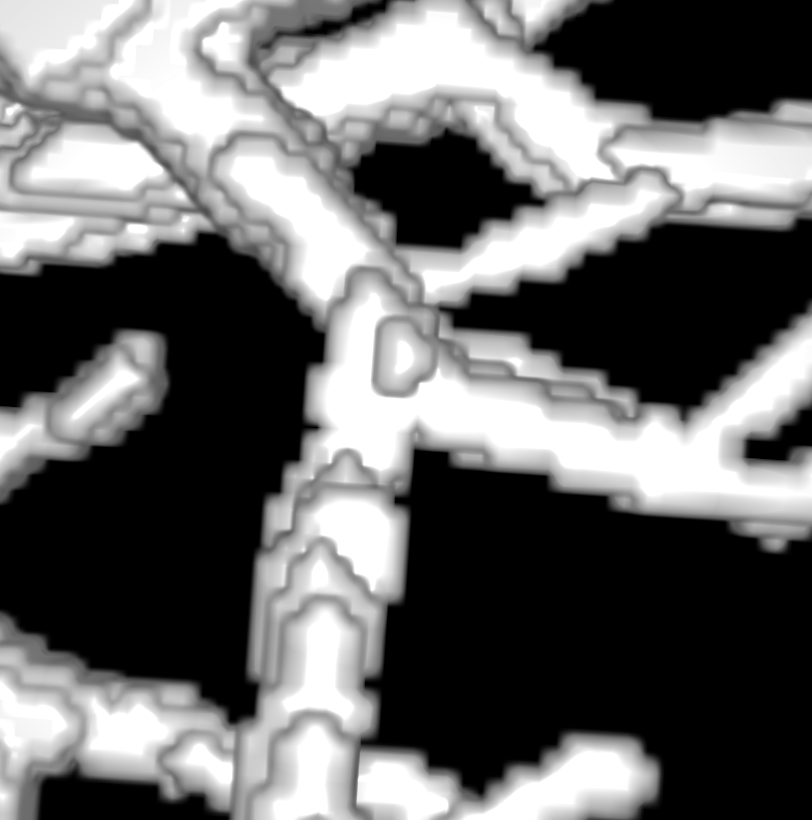
\includegraphics[clip = true, trim  = 0 50 0 80, width=\textwidth]{Images/Ircad_k_GT.png}
        \caption{Vérité terrain}
      \end{subfigure}
      \begin{subfigure}[t]{0.30\textwidth}
        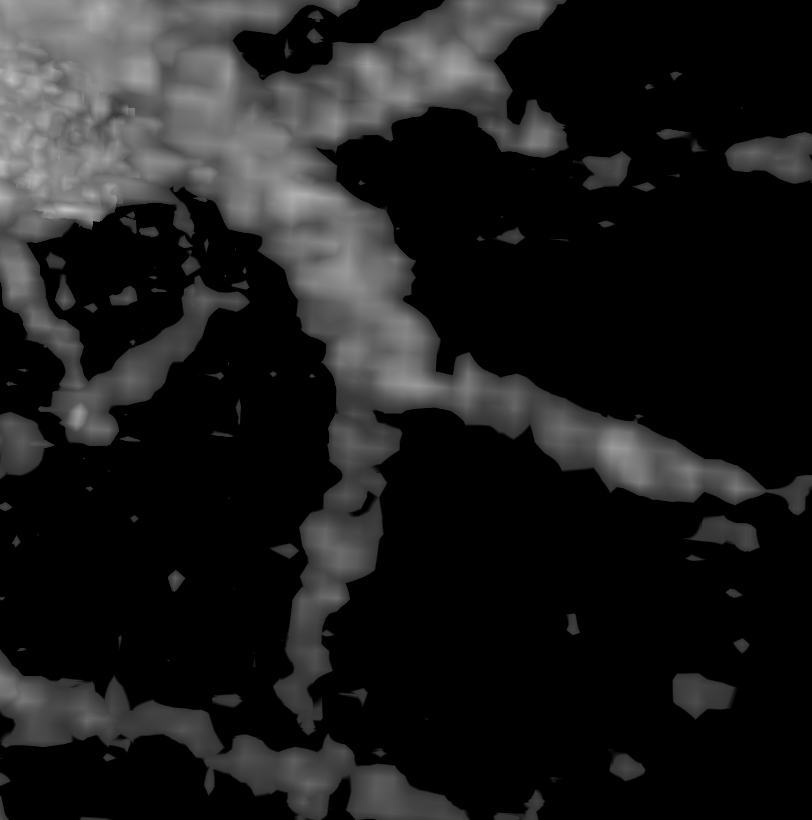
\includegraphics[clip = true, trim  = 0 50 0 80, width=\textwidth]{Images/Ircad_k_Baseline.png}
        \caption{Témoin}
      \end{subfigure}
      \begin{subfigure}[t]{0.30\textwidth}
        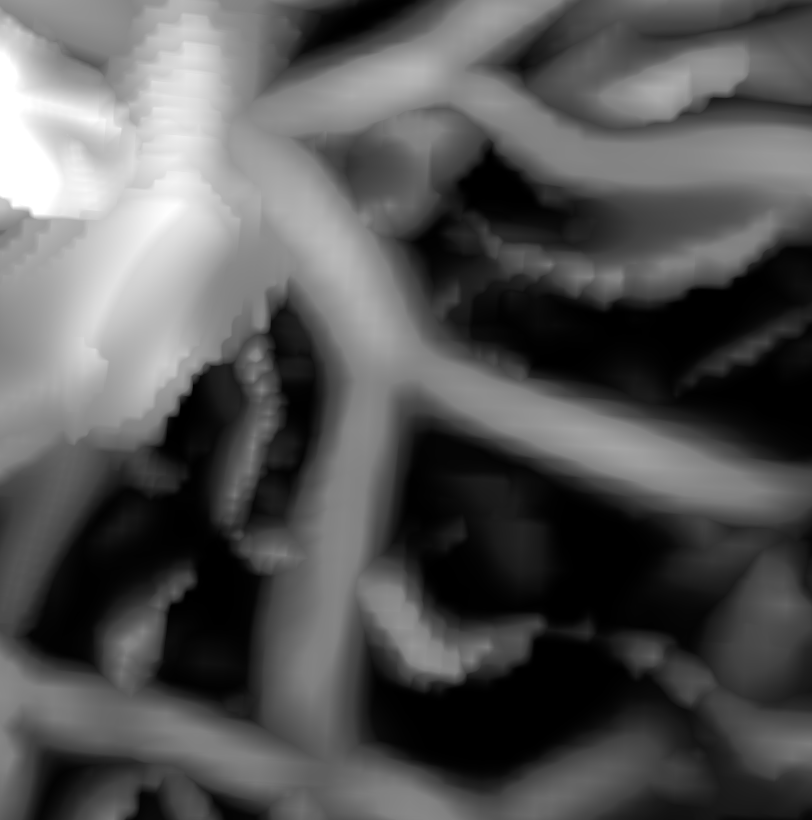
\includegraphics[clip = true, trim  = 0 50 0 80, width=\textwidth]{Images/Ircad_k_Frangi.png}
        \caption{Frangi}
      \end{subfigure}
      \begin{subfigure}[t]{0.30\textwidth}
        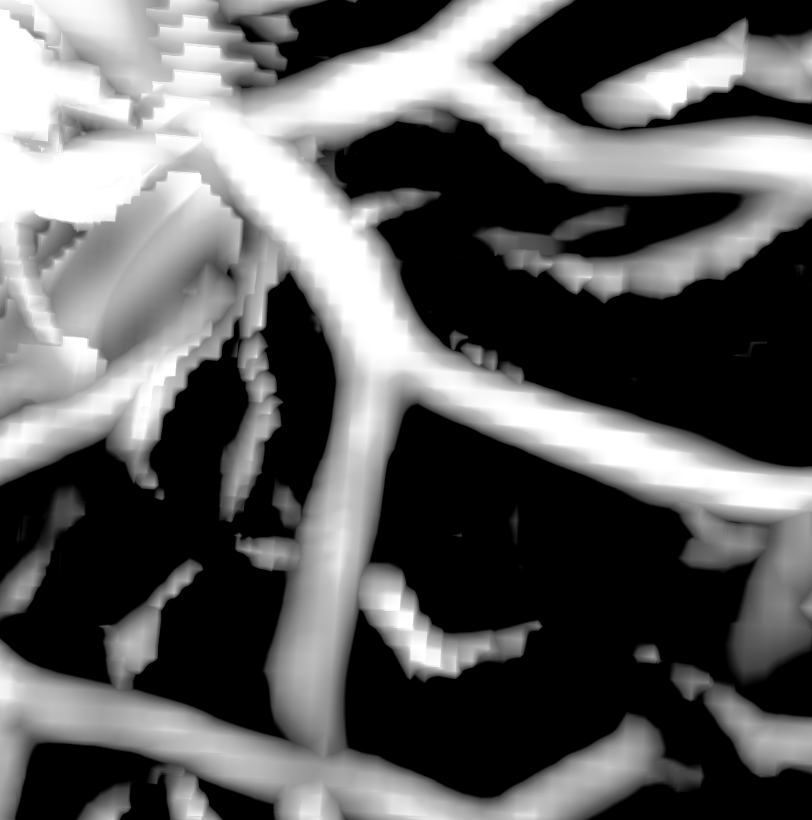
\includegraphics[clip = true, trim  = 0 50 0 80, width=\textwidth]{Images/Ircad_k_Jerman.png}
        \caption{Jerman}
      \end{subfigure}
      \begin{subfigure}[t]{0.30\textwidth}
        \includegraphics[clip = true, trim  = 0 50 0 80, width=\textwidth]{Images/Ircad_k_OOF_GM.png}
        \caption{OOF}
      \end{subfigure}
      \begin{subfigure}[t]{0.30\textwidth}
        \includegraphics[clip = true, trim  = 0 50 0 80, width=\textwidth]{Images/Ircad_k_Meijering.png}
        \caption{Meijering}
      \end{subfigure}
      \begin{subfigure}[t]{0.30\textwidth}
        \includegraphics[clip = true, trim  = 0 50 0 80, width=\textwidth]{Images/Ircad_k_RORPO.png}
        \caption{RORPO}
      \end{subfigure}
      \begin{subfigure}[t]{0.30\textwidth}
        \includegraphics[clip = true, trim  = 0 50 0 80, width=\textwidth]{Images/Ircad_k_Sato.png}
        \caption{Sato}
      \end{subfigure}
      \begin{subfigure}[t]{0.30\textwidth}
        \includegraphics[clip = true, trim  = 0 50 0 80, width=\textwidth]{Images/Ircad_k_Zhang.png}
        \caption{Zhang}
      \end{subfigure}

      \caption{MIP des filtres avec les meilleurs paramètres sur une bifurcation pour le jeu de données de l'Ircad. Le témoin est l'image originale masquée et seuillée de manière optimale par rapport au MCC.
      }
      \label{fig:bifurcation_Ircad}
  \end{figure}
  \begin{figure}[!ht]
    \captionsetup[subfigure]{justification=centering}
    \centering
    \begin{subfigure}[t]{0.30\textwidth}
      \includegraphics[clip = true, trim  =  170 230 150 240, width=\textwidth]{Images/Vascu_2_k_GT.png}
      \caption{Vérité terrain}
    \end{subfigure}
    \begin{subfigure}[t]{0.30\textwidth}
      \includegraphics[clip = true, trim  =  170 230 150 240, width=\textwidth]{Images/Vascu_2_k_Baseline.png}
      \caption{Témoin}
    \end{subfigure}
    \begin{subfigure}[t]{0.30\textwidth}
      \includegraphics[clip = true, trim  =  170 230 150 240, width=\textwidth]{Images/Vascu_2_k_Frangi.png}
      \caption{Frangi}
    \end{subfigure}
    \\
    \begin{subfigure}[t]{0.30\textwidth}
      \includegraphics[clip = true, trim  =  170 230 150 240, width=\textwidth]{Images/Vascu_2_k_Jerman.png}
      \caption{Jerman}
    \end{subfigure}
    \begin{subfigure}[t]{0.30\textwidth}
      \includegraphics[clip = true, trim  =  170 230 150 240, width=\textwidth]{Images/Vascu_2_k_OOF_GM.png}
      \caption{OOF}
    \end{subfigure}
    \begin{subfigure}[t]{0.30\textwidth}
      \includegraphics[clip = true,trim  =  170 230 150 240, width=\textwidth]{Images/Vascu_2_k_Meijering.png}
      \caption{Meijering}
    \end{subfigure}
    \\
    \begin{subfigure}[t]{0.30\textwidth}
      \includegraphics[clip = true, trim  =  170 230 150 240, width=\textwidth]{Images/Vascu_2_k_RORPO.png}
      \caption{RORPO}
    \end{subfigure}
    \begin{subfigure}[t]{0.30\textwidth}
      \includegraphics[clip = true, trim  =  170 230 150 240, width=\textwidth]{Images/Vascu_2_k_Sato.png}
      \caption{Sato}
    \end{subfigure}
    \begin{subfigure}[t]{0.30\textwidth}
      \includegraphics[clip = true, trim  =  170 230 150 240, width=\textwidth]{Images/Vascu_2_k_Zhang.png}
      \caption{Zhang}
    \end{subfigure}

        \caption{MIP des filtres avec les meilleurs paramètres sur une bifurcation pour le jeu de données VascuSynth avec $\sigma=2$. Le témoin est l'image originale masquée et seuillée de manière optimale par rapport au MCC.
        }
      \label{fig:bifurcation_vascu}
  \end{figure}
\begin{figure}[!ht]
  \captionsetup[subfigure]{justification=centering}
      \begin{subfigure}[t]{0.32\textwidth}
          \begin{tikzpicture}
              \node[anchor=south west,inner sep=0] (image) at (0,0) {\includegraphics[clip = true, trim = 40 100 40 70, width=\textwidth]{Images/Bullitt_k_GT.png}};
              \begin{scope}[x={(image.south east)},y={(image.north west)}]
                  \draw[green,thick] (0.33,0.60) rectangle (0.43,0.75);
                  \draw[red,thick] (0.50,0.10) rectangle (0.65,0.35);
              \end{scope}
          \end{tikzpicture}
          \caption{Vérité terrain}
        \end{subfigure}
      \begin{subfigure}[t]{0.32\textwidth}
          \begin{tikzpicture}
              \node[anchor=south west,inner sep=0] (image) at (0,0) {\includegraphics[clip = true, trim = 40 100 40 70,  width=\textwidth]{Images/Bullitt_k_Baseline.png}};
              \begin{scope}[x={(image.south east)},y={(image.north west)}]
                  \draw[green,thick] (0.33,0.60) rectangle (0.43,0.75);
                  \draw[red,thick] (0.50,0.10) rectangle (0.65,0.35);
              \end{scope}
          \end{tikzpicture}
          \caption{Témoin}
        \end{subfigure}
      \begin{subfigure}[t]{0.32\textwidth}
          \begin{tikzpicture}
                  \node[anchor=south west,inner sep=0] (image) at (0,0) {\includegraphics[clip = true, trim = 40 100 40 70,  width=\textwidth]{Images/Bullitt_k_Frangi.png}};
              \begin{scope}[x={(image.south east)},y={(image.north west)}]
                  \draw[green,thick] (0.33,0.60) rectangle (0.43,0.75);
                  \draw[red,thick] (0.50,0.10) rectangle (0.65,0.35);
              \end{scope}
          \end{tikzpicture}
          \caption{Frangi}
        \end{subfigure}
      \begin{subfigure}[t]{0.32\textwidth}
          \begin{tikzpicture}
                  \node[anchor=south west,inner sep=0] (image) at (0,0) {\includegraphics[clip = true, trim = 40 100 40 70,  width=\textwidth]{Images/Bullitt_k_Jerman.png}};
              \begin{scope}[x={(image.south east)},y={(image.north west)}]
                  \draw[green,thick] (0.33,0.60) rectangle (0.43,0.75);
                  \draw[red,thick] (0.50,0.10) rectangle (0.65,0.35);
              \end{scope}
          \end{tikzpicture}
          \caption{Jerman}
        \end{subfigure}
      \begin{subfigure}[t]{0.32\textwidth}
          \begin{tikzpicture}
                  \node[anchor=south west,inner sep=0] (image) at (0,0) {\includegraphics[clip = true, trim = 40 100 40 70,  width=\textwidth]{Images/Bullitt_k_OOF_GM.png}};
              \begin{scope}[x={(image.south east)},y={(image.north west)}]
                  \draw[green,thick] (0.33,0.60) rectangle (0.43,0.75);
                  \draw[red,thick] (0.50,0.10) rectangle (0.65,0.35);
              \end{scope}
          \end{tikzpicture}
          \caption{OOF}
        \end{subfigure}
      \begin{subfigure}[t]{0.32\textwidth}
          \begin{tikzpicture}
                  \node[anchor=south west,inner sep=0] (image) at (0,0) {\includegraphics[clip = true, trim = 40 100 40 70,  width=\textwidth]{Images/Bullitt_k_Meijering.png}};
              \begin{scope}[x={(image.south east)},y={(image.north west)}]
                  \draw[green,thick] (0.33,0.60) rectangle (0.43,0.75);
                  \draw[red,thick] (0.50,0.10) rectangle (0.65,0.35);
              \end{scope}
          \end{tikzpicture}
          \caption{Meijering}
      \end{subfigure}
      \begin{subfigure}[t]{0.32\textwidth}
          \begin{tikzpicture}
                  \node[anchor=south west,inner sep=0] (image) at (0,0) {\includegraphics[clip = true, trim = 40 100 40 70,  width=\textwidth]{Images/Bullitt_k_RORPO.png}};
              \begin{scope}[x={(image.south east)},y={(image.north west)}]
                  \draw[green,thick] (0.33,0.60) rectangle (0.43,0.75);
                  \draw[red,thick] (0.50,0.10) rectangle (0.65,0.35);
              \end{scope}
          \end{tikzpicture}
          \caption{RORPO}
        \end{subfigure}
      \begin{subfigure}[t]{0.32\textwidth}
          \begin{tikzpicture}
                  \node[anchor=south west,inner sep=0] (image) at (0,0) {\includegraphics[clip = true, trim = 40 100 40 70,  width=\textwidth]{Images/Bullitt_k_Sato.png}};
              \begin{scope}[x={(image.south east)},y={(image.north west)}]
                  \draw[green,thick] (0.33,0.60) rectangle (0.43,0.75);
                  \draw[red,thick] (0.50,0.10) rectangle (0.65,0.35);
              \end{scope}
          \end{tikzpicture}
          \caption{Sato}
        \end{subfigure}
      \begin{subfigure}[t]{0.32\textwidth}
          \begin{tikzpicture}
                  \node[anchor=south west,inner sep=0] (image) at (0,0) {\includegraphics[clip = true, trim = 40 100 40 70,  width=\textwidth]{Images/Bullitt_k_Zhang.png}};
              \begin{scope}[x={(image.south east)},y={(image.north west)}]
                  \draw[green,thick] (0.33,0.60) rectangle (0.43,0.75);
                  \draw[red,thick] (0.50,0.10) rectangle (0.65,0.35);
              \end{scope}
          \end{tikzpicture}
          \caption{Zhang}
        \end{subfigure}
      
        \caption{
        MIP des vaisseaux au centre du cerveau pour le jeu de données Bullitt. Ces vaisseaux sont situés sur le même plan, illustrant ainsi les vaisseaux proches (rouge) et les bifurcations (vert).}
      \label{fig:bifurcation_Bullitt}
\end{figure}

Qualitativement, nous observons que les filtres de Frangi et Sato présentent une perte de signal au centre des bifurcations pour l'Ircad et Bullitt et sur les pourtours de la bifurcation pour VascuSynth. Cette perte de signal n'a pas été observée pour les autres filtres. Le déplacement de la perte de signal s'éloignant des bords pour VascunSynth peut s'expliquer par une géométrie particulière pour ce jeu de données. En effet, les nouvelles branches partant d'un vaisseau principal, plus gros, ont une épaisseur plus réduite. Le centre de la bifurcation se retrouve translaté de l'intersection des deux vaisseaux à la base du plus petit. Concernant les vaisseaux adjacents, certains filtres ont une tendance à fusionner les vaisseaux très proches. Ces filtres sont Jerman, Meijering et Zhang. Les autres filtres tels que Frangi, Sato, OOF et RORPO semblent plus robustes à cet effet. En particulier, cette robustesse est assurée par la propriété d'anti-extensivité pour RORPO.
\begin{table}[!ht]
  \caption{Résultats quantitatifs (moyenne $\pm$ écart-type) pour le masque des bifurcations \maskbif sur l'ensemble des jeux de données. Seul le Dice est exprimé car le MCC n'est pas défini sur ce masque.}
  \label{tab:dice_bif}
  \resizebox{\textwidth}{!}{
  \begin{tabular}{lccccc}
            \hline
            & \multicolumn{5}{c}{Dice} \\
            \hline
            & Ircad & Bullitt & VascuSynth 2 & VascuSynth 4 & VascuSynth 6 \\
            \hline
  Témoin  & $ 0.657 \pm 0.142 $ & $ 0.492 \pm 0.091 $ & $ 0.408 \pm 0.256 $ & $ 0.382 \pm 0.255 $ & $ 0.360 \pm 0.243 $ \\
  Frangi    & $ 0.732 \pm 0.138 $ & $ \tbf{0.797} \pm 0.039 $ & $ 0.716 \pm 0.043 $ & $ 0.783 \pm 0.051 $ & $ \tbf{0.833} \pm 0.057 $ \\
  Jerman    & $ 0.632 \pm 0.161 $ & $ 0.748 \pm 0.056 $ & $ 0.713 \pm 0.061 $ & $ 0.652 \pm 0.042 $ & $ 0.562 \pm 0.050 $ \\
  Meijering & $ \tbf{0.881} \pm 0.096 $ & $ 0.716 \pm 0.084 $ & $ \tbf{0.904} \pm 0.048 $ & $ \tbf{0.875} \pm 0.044 $ & $ 0.810 \pm 0.053 $ \\
  OOF       & $ 0.728 \pm 0.132 $ & $ 0.779 \pm 0.069 $ & $ 0.666 \pm 0.047 $ & $ 0.604 \pm 0.055 $ & $ 0.543 \pm 0.062 $ \\
  RORPO     & $ 0.616 \pm 0.168 $ & $ 0.758 \pm 0.031 $ & $ 0.658 \pm 0.098 $ & $ 0.563 \pm 0.105 $ & $ 0.440 \pm 0.119 $ \\
  Sato      & $ 0.652 \pm 0.145 $ & $ 0.717 \pm 0.049 $ & $ 0.671 \pm 0.042 $ & $ 0.684 \pm 0.060 $ & $ 0.593 \pm 0.056 $ \\
  Zhang     & $ 0.646 \pm 0.165 $ & $ 0.781 \pm 0.051 $ & $ 0.635 \pm 0.056 $ & $ 0.600 \pm 0.053 $ & $ 0.678 \pm 0.070 $
  \end{tabular}
  }
  \end{table}

Nous divisons l'analyse quantitative (Tab. \ref{tab:dice_bif}) en deux parties avec d'une part les jeux de données réels et d'autre part les données synthétiques dont la vérité terrain des bifurcations est plus précise.
\paragraph{Ircad}
Pour l'Ircad, les trois filtres qui ont le Dice le plus élevé sont Meijering (Dice=$0.881$), Frangi (Dice=$0.732$), OOF (Dice=$0.728$). Dans ce jeu de données, la majorité des vaisseaux est plus intense que le fond, ce qui permet au témoin d'obtenir un Dice élevé (Dice=$0.657$). Les deux filtres présentant les moins bonnes performances sont Jerman (Dice=$0.632$) et RORPO (Dice=$0.616$). Sur ce jeu de données, les performances des filtres suivent les mêmes tendances que sur \maskvascular. Seuls Meijering et OOF présentent des résultats bien plus élevés pour les bifurcations que pour \maskvascular.
\paragraph{Bullitt}
Les filtres montrant les meilleurs performances sur le jeu de données Bullitt sont Frangi (Dice=$0.797$), Zhang (Dice=$0.781$) et OOF (Dice=$0.779$). Sato (Dice=$0.717$) et Meijering (Dice=$0.716$) sont les deux filtres présentant les résultats les plus faibles pour les bifurcations de Bullitt. 

Frangi et OOF sont les deux filtres présentant des résultats supérieurs aux autres filtres sur les deux jeux réels. Le comportement des autres filtres est difficile à définir et la corrélation avec les résultats visuels n'est pas évidente. Toutefois, les valeurs des métriques obtenues sur \maskbif suivent les tendances observées sur \maskvascular.
\paragraph{VascuSynth}
Pour VascuSynth, Frangi et Meijering sont les filtres avec les valeurs de Dice les plus hautes (Dice=$0.716$ vs. Dice=$0.904$ pour $\sigma=2$), (Dice=$0.783$ vs. Dice=$0.875$ pour $\sigma=4$), (Dice=$0.833$ vs. Dice=$0.810$ pour $\sigma=6$). Frangi et Zhang sont les filtres dont les performances ne décroissent pas alors que le bruit augmente.
Encore une fois, les résultats avec les bifurcations sont corrélés avec le rehaussement dans le voisinage des vaisseaux. Par exemple, la dégradation des résultats de RORPO avec l'augmentation du niveau de bruit s'observe également pour les bifurcations.
\section{Discussion}
\subsection{Recommandations sur l'usage des filtres}
En se basant sur ces résultats d'expériences, il est possible de formuler quelques recommandations en fonction du masque de région d'intérêt.
\subsubsection*{Meijering}
 Nous avons observé que les performances de Meijering sont faibles sur les jeux de données réels, car le filtre rehausse fortement le bruit. Ce comportement est consistant avec le fait que Meijering est un filtre dédié au rehaussement dans des images très faiblement contrastées pour des applications de tracking. Il faut toutefois noter que Meijering présente de bons résultats sur les données synthétiques de VascuSynth. Il peut être intéressant d’appliquer Meijering dans plusieurs contextes :
\begin{itemize}
  \item les images sont faiblement contrastées et présentent une géométrie des vaisseaux relativement droite sans variations de diamètres ;
  \item l'utilisateur choisit d'appliquer une segmentation basée sur une stratégie de tracking et/ou applique une stratégie de post-traitement capable d'identifier les faux positifs.
\end{itemize}
\subsubsection*{OOF}
OOF, couplé avec la mesure de tubularité de la moyenne géométrique, présente des résultats relativement faibles sur les jeux de données, ce qui peut s'expliquer par deux éléments : (1) le choix de la mesure dont le pouvoir de discrimination entre les plateaux et les structures tubulaires est faible ; et (2) OOF est basé sur l'hypothèse de sections de vaisseaux à géométrie circulaire, ce qui en pratique n'est pas toujours le cas, en particulier pour l'Ircad. Il convient aussi de noter que OOF est un cadre d'espace d'échelles et que différentes mesures de tubularité peuvent être utilisées en fonction de l'application d'intérêt. OOF est un bon choix dans les cas suivants : 
\begin{itemize}
  \item les vaisseaux présentent des sections circulaires ;
  \item les réseaux vasculaires présentent un nombre important de vaisseaux adjacents.
\end{itemize}
\subsubsection{Sato et Frangi}
Sato et Frangi présentent tous les deux de bonnes performances dans notre banc de test. Ces deux filtres proposent un bon compromis entre sensibilité et spécificité, mais produisent la plupart du temps une perte de signal au niveau des bifurcations. Nous recommandons Frangi dans les cas suivants :
\begin{itemize}
  \item les vaisseaux dans les images ont des diamètres supérieurs à quelques voxels ;
  \item l'utilisateur a besoin d'un contrôle efficace sur le niveau de bruit à filtrer, au prix de la perte des petits vaisseaux ;
  \item \newV{le rehaussement des bifurcations est un facteur déterminant de la méthode de segmentation ;}
  \item \newV{un filtrage du bruit est nécessaire.}
\end{itemize}
Sato est recommandé dans les cas suivants :
\begin{itemize}
  \item les images présentent peu de bruit ;
  \item les vaisseaux ont des sections circulaires ;
  \item les réseaux vasculaires comportent des vaisseaux adjacents.
\end{itemize}
\subsubsection*{Jerman}
Jerman présente de bonnes performances avec une sensibilité importante et rehausse nettement les contours de vaisseaux. Cependant, le filtre a tendance à être plus sensible au bruit que les filtres hessiens classiques (i.e. Frangi et Sato) et partage la même tendance à surestimer le volume des vaisseaux. Nous recommandons le filtre de Jerman dans les cas suivants : 
\begin{itemize}
\item les images présentent des vaisseaux fins et peu contrastés ;
\item le niveau de bruit des images est faible.
\end{itemize}
\subsubsection*{Zhang}
Zhang est une version modifiée de Jerman, créé pour être moins sensible aux artefacts de bord. Malheureusement la méthode est limitée à des organes spécifiques (ici le  foie). Bien que la méthode propose des résultats intéressants, celle-ci requiert une connaissance a priori de la distribution des intensités des structures de l'image seulement disponible pour certaines applications. Zhang est un bon filtre dans les cas suivants :
\begin{itemize}
\item les applications où un masque des organes d'intérêt est disponible ;
\item La distribution des intensités des vaisseaux se mélange peu avec la distribution d'intensité des autres tissus.
\end{itemize}
\subsubsection*{RORPO}
RORPO obtient la première place dans les deux jeux de données réels sur le masque global, mais produit des résultats faibles pour le jeu de données synthétiques VascuSynth. Le filtre différencie de manière efficace les bords des organes et les structures tubulaires et ne surestime jamais la taille des vaisseaux. Cependant, RORPO favorise la spécificité par rapport à la sensibilité et de ce fait présente un plus grand nombre de faux négatifs que les autres méthodes. RORPO est un bon choix pour les applications suivantes~:
\begin{itemize}
  \item les applications nécessitant la détection des contours précis des vaisseaux ;
  \item les applications où il est important de minimiser le nombre de faux positifs. 
\end{itemize}
\subsection{Influence des paramètres}
Nous avons voulu aller plus loin dans l'analyse des filtres en détaillant l'influence de leurs paramètres. Nous discutons d'abord des paramètres d'échelles puis des paramètres intrinsèques. Pour ces derniers, nous nous sommes intéressés à la variation du MCC pour l'ensemble des jeux de paramètres testés ainsi qu'à la visualisation des types de structures rehaussés pour les paramètres optimaux de chaque filtre. L'ensemble des paramètres optimaux obtenus lors de nos expériences sont résumés dans la table \ref{tab:optimal_parameters}.
\begin{table}[!ht]
  \begin{center}
  \caption{Paramètres optimaux des 7 filtres dans les 3 jeux de données.}
      \begin{tabular}{llrrrrr}
                          \hline
             & Paramètres  & Ircad       &  \multicolumn{3}{c}{VascuSynth}            &  Bullitt\\
             &   &         & $\sigma = 2$  & $\sigma = 4$ & $\sigma = 6$ &       \\
                         \hline
      Frangi &  $\alpha$  & $1$         & $0.2$     & $0.2$        & $0.2$           & $1.0$   \\
      ---    &  $\beta$   & $1$         & $0.6$     & $0.4$       & $0.4$           & $0.4$   \\
      ---    &  $C$       & $30$        & $30$       & $30$         & $30$            & $30$    \\
      Jerman & $\tau$     & $0.1$       & $0.2$     & $0.2$       & $0.3$          & $0.2$  \\
      OOF &  $\sigma$     & $1$         & $0.1$      & $0.1$        & $0.1$           & $0.1$   \\
      RORPO  & Échelles min.  & $70$        & $50$       & $50$         & $40$            & $20$    \\
      ---    & Facteur      & $1.3$       & $1.1$     & $1.2$       & $1.4$          & $1.3$  \\
      ---    &  Nb échelles  & $4$         & $3$        & $2$          & $2$             & $4$     \\
      Sato   & $\alpha_1$ & $0.3$       & $0.3$      & $0.3$        & $0.5$          & $0.7$   \\
      ---   & $\alpha_2$ & $1.6$       & $2$      & $1$        & $2$           & $1.0$   \\
      Zhang  & $\tau$     & $0.3$       & $0.4$     & $0.8$       & $0.9$          & $0.1$  \\
          \hline
      \end{tabular}
  \label{tab:optimal_parameters}
  \end{center}
\end{table}
\subsubsection{Influence des paramètres d'échelles}
Les choix des paramètres d'échelles sont déterminants pour l'ensemble des filtres. Lorsque la technique de rehaussement est efficace, les variations du résultat entre une échelle non optimisée et une échelle optimisée sont très importantes. Entre le moins bon et le meilleur jeu de paramètres (étape 1 de l'optimisation), des variations de MCC entre $0.23$ et $0.30$ ont été observées pour les filtres hessiens. Pour RORPO, dont le paramétrage repose exclusivement sur la taille des éléments structurants, une variation moyenne de $0.18$ du MCC a été observée. OOF présente le delta le plus faible, avec des variations de MCC moyennes de $0.07$. Une hypothèse est que la majeure partie des vaisseaux sont capturés dans une seule échelle, limitant ainsi l'impact de l'optimisation.
\subsubsection{Influence des paramètres intrinsèques}
Nous proposons d'étudier l'influence des paramètres intrinsèques de deux manières : en observant les variations de MCC obtenues sur l'ensemble des jeux de paramètres d'un filtre et en analysant la réponse théorique des filtres pour leurs paramètres optimaux. 
\subsubsubsection{Rehaussement théorique}
\newV{Nous avons vu dans le chapitre \chapSOTAN{} que pour les filtres à descripteurs matriciels, la mesure de tubularité était définie à partir d'un triplet de valeurs propres. Ces valeurs propres expriment les variations d'intensité locale et peuvent être associées à des géométries particulières (Sec. \chapSOTAN{}, Fig. \ref{sec:mesure_tubularity}). Par exemple, une structure tubulaire est définie par deux valeurs propres élevées et une valeur propre proche de zéro. Une structure planaire est définie par deux valeurs propres proches de zéro et une valeur propre élevée. Une structure sphérique est définie par les trois valeurs propres égales.}

\newV{La figure \ref{fig:exemple_geometry} définit un ensemble de triplets de valeurs propres qui varient entre $-1$ et $-5$. Dans cet espace, les points $(-5,-5,-1)$,$(-1,-5,-5)$ et $(-5,-1,-5)$ correspondent à une géométrie tubulaire. Les points $(-1,-5,-1)$,$(-1,-1,-5)$ et $(-5,-1,-1)$ correspondent à une géométrie planaire. Les points situés sur la diagonale formée par les points $(-1,-1)$ et $(-5,-5)$ correspondent à une géométrie sphérique. Le reste des points forment une combinaison linéaire de ces 3 cas particuliers.}

\newV{Sur cet espace, on peut calculer la valeur du rehaussement, représentée par une couleur, pour chaque triplet de valeurs propres. On construit ainsi une signature visuelle qui permet de caractériser le rehaussement pour un jeu de paramètres donné.}
\begin{figure}[!ht]
  \centering
  \includegraphics[height=8cm]{Images/eigen_meaning_3.png}
  \caption{Correspondance entre géométrie et valeurs propres. Les valeurs propres sont représentées par un triplet de flèches en chaque point. Les structures décrites par les valeurs propres sont représentées par des ellipses de couleurs. Trois régions correspondent à des géométries caractéristiques : la géométrie tubulaire en bleu, la géométrie planaire en vert foncé et la géométrie sphérique en rouge. Les autres régions en vert correspondent à des interpolations de ces trois géométries.}
  \label{fig:exemple_geometry}
\end{figure}
\subsubsubsection{Frangi}
Pour Frangi, la différence de MCC entre le meilleur et le moins bon jeu de paramètres intrinsèque est de $0.30$. Cette différence est la plus marquée parmi l'ensemble des filtres.

\newV{Ce résultat était prévisible, car les paramètres de la mesure de tubularité de Frangi modulent la réponse du filtre pour une diversité importante de géométrie. Cette modulation est beaucoup plus importante que pour les autres filtres. On observe cependant que des combinaisons de jeux de paramètres assez éloignées produisent des résultats assez similaires en termes de MCC. Par exemple les paramètres $\{\alpha=0.4$, $\beta=1\}$, $C=30$, $\alpha=0.6$, $\beta=1.0$, $C=30$ et $\{\alpha=1,\beta=0.4,C=30\}$ produisent des MCC moyens sur l'Ircad de $0.342$, $0.351$ et $0.351$. On obtient donc des résultats quantitatifs similaires avec des valeurs de suppression de blobs et de plateaux différents. On peut illustrer ces plateaux de jeux de paramètres en représentant l'ensemble de l'espace des paramètres intrinsèques en fonction du MCC moyen associé, ce que nous illustrons figure \ref{fig:frangi_params}. }
\begin{figure}[!ht]
  \centering
  \includegraphics[width=\textwidth]{Images/frangi_params.png}
  \caption{Valeur du MCC moyen associé aux jeux de paramètres intrinsèques de Frangi pour la base de l'Ircad. À gauche, représentation de l'ensemble des paramètres intrinsèques testés sur le jeu de données. Chaque point représente un jeu de paramètres $\{\alpha,\beta, C\}$ auquel est associé une couleur représentant le MCC moyen. À droite, représentation des mêmes jeux de paramètres sous la forme de surfaces. Chaque surface est définie par l'ensemble des variations d'$\alpha$ et $\beta$ pour un C donné. L'élévation des vertices de la surface correspond au MCC moyen pour un jeu de paramètres donné. Cette représentation illustre les plateaux de performances liés aux paramètres intrinsèques du filtre de Frangi.}
  \label{fig:frangi_params}
\end{figure}

\newV{En moyenne, une variation de MCC de $0.2$ a été observée entre les paramètres par défaut proposés par Frangi et les paramètres optimisés. D'un point de vue géométrique, les paramètres par défaut ($\alpha=0.5$, $\beta=0.5$) correspondent à un modèle de tubularité modéré qui autorise des variations planaires et sphériques des structures (Fig. \ref{fig:exemple_geometry_frangi}). Pour Bullitt dont les vaisseaux sont circulaires et fins, les paramètres optimisés correspondent à un modèle de tubularité beaucoup plus strict sans variations de géométrie (Fig. \ref{fig:exemple_geometry_frangi} (a)). Les paramètres optimaux pour vascuSynth $\sigma = 2$ sont similaires aux paramètres par défaut en relâchant encore plus la contrainte de tubularité (Fig. \ref{fig:exemple_geometry_frangi} (d)). L'Ircad est la base qui présente le plus de variations de formes de vaisseaux. Les paramètres optimaux pour l'Ircad sont ceux qui diffèrent le plus des paramètres par défaut. Ils favorisent les structures tubulaires et les structures sphériques aux valeurs propres élevées (Fig. \ref{fig:exemple_geometry_frangi} (c)).}
\begin{figure}[!ht]
  \captionsetup[subfigure]{justification=centering}
  \centering
  \begin{subfigure}[t]{0.45\textwidth}
    \centering
    \includegraphics[width=\textwidth]{Images/Frangi_default_P.png}
    \caption{Paramètres par défaut}
  \end{subfigure}
  \begin{subfigure}[t]{0.45\textwidth}
    \centering
    \includegraphics[width=\textwidth]{Images/Bullitt_Frangi_BP.png}
    \caption{Bullitt}
  \end{subfigure}
  \begin{subfigure}[t]{0.45\textwidth}
    \centering
    \includegraphics[width=\textwidth]{Images/Ircad_Frangi_BP.png}
    \caption{Ircad}
  \end{subfigure}
  \begin{subfigure}[t]{0.45\textwidth}
    \centering
    \includegraphics[width=\textwidth]{Images/Vascu_2_Frangi_BP.png}
    \caption{VascuSynth $\sigma=2$}
  \end{subfigure}
  \caption{Visualisation de la réponse théorique du filtre de Frangi pour les paramètres optimaux du banc de test (Tab. \ref{tab:optimal_parameters}). Les paramètres par défaut proposé par Frangi sont présentés à titre indicatif (a). Pour Bullitt (b) et VascuSynth (c), les paramètres optimaux ont une réponse proche des paramètres par défaut. Pour l'Ircad (d), les paramètres optimaux favorisent la détection de structures plus arrondies.}
  \label{fig:exemple_geometry_frangi}
\end{figure}
\subsubsection{Jerman et Zhang}
Les filtres de Jerman et Zhang présentent de très faibles variations de MCC autour de $0.04$ entre le moins bon et le meilleur jeu de paramètres. Ceci est probablement causé par le seuillage automatique qui compense l'effet du paramètre $\tau$, dont le rôle est de contrôler l'homogénéité de la réponse du filtre. Les filtres de Jerman et Zhang sont caractérisés par une relaxation importante du modèle tubulaire avec un rehaussement marqué aussi bien pour les structures tubulaires que sphériques et planaires (Fig. \ref{fig:exemple_geometry_jerman}). Une faible valeur de $\tau$ comme pour l'Ircad rehausse aussi les structures dont les valeurs propres sont faibles, et notamment le bruit.
\begin{figure}[!ht]
  \captionsetup[subfigure]{justification=centering}
  \centering
  \begin{subfigure}[t]{0.45\textwidth}
    \centering
    \includegraphics[width=\textwidth]{Images/Bullitt_Jerman_BP.png}
    \caption{Bullitt}
  \end{subfigure}
  \begin{subfigure}[t]{0.45\textwidth}
    \centering
    \includegraphics[width=\textwidth]{Images/Bullitt_Jerman_BP.png}
    \caption{VascuSynth $\sigma = 2$}
  \end{subfigure}
  
  \begin{subfigure}[t]{0.45\textwidth}
    \centering
    \includegraphics[width=\textwidth]{Images/Ircad_Jerman_BP.png}
    \caption{Ircad }
  \end{subfigure}
  \caption{Visualisation de la réponse théorique du filtre de Jerman (couleur) pour les paramètres optimaux de Bullitt, VascuSynth $\sigma=2$ et l'Ircad. Le rehaussement est plus homogène et accepte des structures tubulaires de géométries plus variées qu'un filtre comme Frangi ou Sato.}
  \label{fig:exemple_geometry_jerman}
\end{figure}
\subsubsection{Sato}
Le filtre de Sato présente très peu de variations par jeu de paramètres, avec une variation maximale moyenne de MCC de 0.02. Les paramètres par défaut proposés par Sato, sont donc très proches des paramètres optimaux trouvés. D'un point de vue géométrique, Sato propose une mesure assez stricte par rapport à la définition de la tubularité, avec une réponse forte pour les tubes. En particulier, le paramètre $\alpha_1$ contrôle la relaxation du modèle par rapport aux blobs/bifurcations (Fig. \ref{fig:exemple_geometry_Sato}).
\begin{figure}[!ht]
  \captionsetup[subfigure]{justification=centering}
  \centering
  \begin{subfigure}[t]{0.45\textwidth}
    \includegraphics[width=\textwidth]{Images/Bullitt_Sato_BP.png}
    \caption{Bullitt}
  \end{subfigure}
  \begin{subfigure}[t]{0.45\textwidth}
    \includegraphics[width=\textwidth]{Images/Ircad_Sato_BP.png}
    \caption{Ircad}
  \end{subfigure}
  
  \begin{subfigure}[t]{0.45\textwidth}
    \includegraphics[width=\textwidth]{Images/Ircad_Sato_BP.png}
    \caption{VascuSynth}
  \end{subfigure}
  \caption{Visualisation de la réponse du filtre de Sato (couleur) pour les paramètres optimaux de Bullitt, l'Ircad et VascuSynth $\sigma=2$. Le rehaussement est plus strict en limitant le rehaussement à des variations plus faibles de la géométrie.}
  \label{fig:exemple_geometry_Sato}
\end{figure}

Il convient aussi de noter que dans nos expériences, la plupart des paramètres optimaux des filtres ne sont pas choisis en fonction de leur capacité à produire une réponse forte en valeur absolue, mais à différencier les structures en valeurs relatives. On remarque ainsi que dans notre expérience, la plupart des rehaussements ont des valeurs souvent basses. Ces faibles valeurs de rehaussement sont compensées par la sélection du seuil optimal de binarisation. \newV{Pour une utilisation pratique, et donc sans vérité terrain disponible, on peut avoir recours à un seuil de décision fixe plutôt que variable. Dans ce cas, la recherche d'un rehaussement élevé en valeur absolue devient une contrainte supplémentaire d'optimisation des paramètres. Il est donc probable que les paramètres optimaux soient différents dans ces conditions. Dans notre banc de test actuel, vérifier cette hypothèse serait possible en optimisant les paramètres des filtres par rapport au PSNR plutôt qu'au MCC calculé sur la réponse binaire des filtres.}
\subsection{Temps de calcul des filtres}
Le temps de calcul moyen pour chaque filtre sur trois volumes de chaque jeu de données est présenté dans la table \ref{tab:Computation time benchmark}. Tous les filtres hessiens sont similaires (environ 1 minute par volume), excepté pour Zhang puisque l'étape de K-moyenne induit un surcoût calculatoire.
\begin{table}
  \centering
  \caption{Temps de calcul des 7 filtres (temps CPU en secondes). Moyenne effectuée sur 3 volumes de chaque jeu de données.}
  \label{tab:Computation time benchmark}
  \begin{tabular}{lrrr}
  \hline
                     & Ircad      & Bullit  & VascuSynth \\
                     \hline
  Frangi    & ~~~~~~~~~$72$  & ~~~~~~~~~$47$   & ~~~~~~~~~$6$   \\
  Sato      & $67$  & $44$   & $\tbf{5}$   \\
  Meijering & $43$  & $36$   & $6$   \\
  OOF       & $231$  & $274$   & $17$   \\
  RORPO     & $1776$  & $1227$   & $160$   \\
  Jerman    & $\tbf{39}$  & $\tbf{34}$   & $6$   \\
  Zhang     & $106$  & $80$   & $10$  \\
  \hline
  \end{tabular}
\end{table}

OOF et RORPO requièrent beaucoup plus de puissance de calcul puisque leur complexité n'est pas linéaire par rapport à la taille de l'image. Cependant, l'implémentation de RORPO est parallélisée pour réduire le temps de calcul. OOF peut être implémenté sur GPU comme démontré par Law et al. \cite{Law2009_efficient_implementation} afin de réduire son temps de calcul.
\section{Bilan}
Dans ce chapitre, nous avons analysé sept filtres de rehaussement. Cette analyse repose à la fois sur les comparaisons des performances entre les filtres et la comparaison des performances de différents jeux de paramètres. 

Nous avons exposé des différences notables entre les filtres dans leur capacité à rehausser le réseau vasculaire dans son ensemble, mais aussi à rehausser des parties spécifiques du réseau, tels que les vaisseaux fins. Nous avons aussi montré que leur performance peut varier significativement en présence de bruit. De plus, nous avons exposé les différentes faiblesses des filtres par rapport à leur réponse au niveau des bords des organes.

Nous avons également démontré l'importance de la paramétrisation de l'espace d'échelles des filtres qui influe de manière significative sur la capacité des filtres à capturer l'ensemble des tailles de vaisseaux présents. Pour les paramètres intrinsèques, nous avons montré qu'ils jouaient, eux aussi, un rôle dans les performances des filtres. En effet, une mauvaise paramétrisation de ces paramètres peut faire chuter les performances des filtres de manière importante. Cette chute de performance est d'autant plus marquée dans des situations réelles lorsque choisir un seuil optimal après le rehaussement est particulièrement complexe. Cependant, dans un certain nombre de cas, des performances similaires peuvent être atteintes par un ensemble de jeux de paramètres. Ce type de plateau justifie l'utilisation de paramètres "par défaut" proposés par les auteurs des méthodes.   

En tant que filtre sans paramètre intrinsèque, Meijering est le plus simple des filtres à paramétrer. RORPO et OOF sont aussi simples à paramétrer puisque RORPO n'a qu'un seul paramètre intrinsèque binaire (le paramètre de dilatation) et OOF dépend seulement d'un paramètre de lissage $\sigma$. Jerman et Zhang ont, eux aussi, un seul paramètre intrinsèque à régler, $\tau$, qui contrôle à la fois la netteté des bordures des vaisseaux et l'homogénéité du contraste. Dans la plupart des cas, le $\tau$ optimal est faible de manière à obtenir une réponse homogène. 

Sato et Frangi sont les filtres les plus complexes à paramétrer. Ils possèdent $2$ et $3$ paramètres intrinsèques pour lesquels la correspondance avec la réalité physique des images est difficile à déterminer. Ces paramètres influencent directement la géométrie des structures et le résultat est donc sensible au changement de paramètres. Nous avons pu observer que les paramètres optimaux pour les deux filtres étaient choisis de manière à relaxer la contrainte de tubularité et rehausser les vaisseaux aux formes plus variés. Cependant, le gain de performances n'est pas significatif par rapport aux paramètres par défaut recommandés par les auteurs.

\newV{Pour les bifurcations, nos observations quantitatives ne sont pas toujours en accord avec nos observations qualitatives. Le rehaussement sur les bifurcations est soit similaire, soit d'un ordre de grandeur plus élevé que le rehaussement sur les autres régions. Par exemple le filtre de Frangi montre des performances quantitatives élevées dans l'ensemble des jeux de données. Ces résultats contredisent en partie les observations de perte de signal observées visuellement sur le filtre de Frangi ou le filtre de Sato. On peut toutefois remarquer que les mesures obtenues sur les bifurcations s'alignent la plupart du temps sur les résultats obtenus pour le masque du voisinage des vaisseaux. Il est donc possible que les seuils de binarisation choisis pour les paramètres optimaux des filtres compensent les éventuelles pertes de signal.}

Enfin, il est important que noter que le résultat de ces expériences dépend des jeux de données et des vérités terrain associées. Les jeux de données publics sont rares et donc précieux, même s'ils présentent des limitations. En particulier, les vérités terrain de l'Ircad n'incluent pas certains vaisseaux larges, ce qui influence les métriques calculées. De plus, le diamètre des vaisseaux est souvent surestimé, ce qui ajoute un biais systématique (positif ou négatif en fonction des méthodes) dans les résultats quantitatifs. Le jeu de données VascuSynth étant synthétique, la géométrie des vaisseaux est plus simple que pour les vaisseaux réels, ce qui impacte le résultat des filtres. De plus, l'environnement dans lequel sont les vaisseaux est plus simple que dans la plupart des images médicales, qui contiennent d'autres structures et organes.



